\documentclass{beamer}
 
\usepackage[utf8]{inputenc}
\usepackage{etoolbox}
\setbeamercovered{transparent}

% \usepackage{bm}
\usepackage{mathtools}          %loads amsmath as well
\usepackage{amssymb}
\usepackage{lmodern}
\usepackage{flexisym}
\usepackage{graphicx}
\usepackage[absolute,overlay]{textpos}




\usepackage{tikz}
\usetikzlibrary{positioning}
\usetikzlibrary{arrows}
\usetikzlibrary{shapes}
\usetikzlibrary{decorations.pathreplacing}

\tikzstyle{inputNode}=[draw,circle,minimum size=10pt,inner sep=0pt]
\tikzstyle{stateTransition}=[-stealth, thick]

\tikzset{basic/.style={draw,fill=blue!20,text width=1em,text badly centered}}
\tikzset{input/.style={basic,circle}}
\tikzset{weights/.style={basic,rectangle}}
\tikzset{functions/.style={basic,circle,fill=blue!10}}
\tikzset{
  treenode/.style = {shape=rectangle, rounded corners,
                     draw, align=center,
                     top color=white, bottom color=blue!20},
  root/.style     = {treenode, font=\Large, bottom color=green!30},
  env/.style      = {treenode, font=\ttfamily\normalsize},
  dummy/.style    = {circle,draw}
  invisible/.style={opacity=0},
  visible on/.style={alt={#1{}{invisible}}},
  alt/.code args={<#1>#2#3}{%
      \alt<#1>{\pgfkeysalso{#2}}{\pgfkeysalso{#3}} % \pgfkeysalso doesn't change the path
  },
}

% \usetheme{Copenhagen}
\usetheme{EastLansing}
\usecolortheme{dolphin}
 
 
%Information to be included in the title page:

\titlegraphic{%
    \vspace*{10mm}
    \makebox[0.9\paperwidth]{%
        \raggedleft
\includegraphics[height=1.1cm,keepaspectratio]{pics/oeaw-logo.jpg}%
        \hfill%
        % \hspace*{-10mm}
        \raggedright
\includegraphics[height=1.1cm,keepaspectratio]{pics/smi-logo.jpg}%
        % \hspace*{3mm}
    }%
}

\title[Introduction to Machine learning] %optional
{Machine learning methods applied to the analysis of central exclusive production events in ALICE}
 
% \subtitle{A short story}
  
\author[Ratzenböck] % (optional, for multiple authors)
{Sebastian Ratzenböck\inst{1}}

\institute[SMI] % (optional)
{
\inst{1}%
Stefan Meyer Institut\\
Österreichische Akademie der Wissenschaften
}
  
\date[26.April 2018] % (optional)
{26. April 2018}
 
\begin{document}

%------------------------------------------------ 
\frame{\titlepage}

%------------------------------------------------ 

\begin{frame}
    \frametitle{Outline}
    \tableofcontents
\end{frame}

%------------------------------------------------ 

\begin{frame}
    \frametitle{Introduction}
    \centering\begin{tikzpicture}
        \node[inner sep=0pt] (diffr) at (0,0)
            {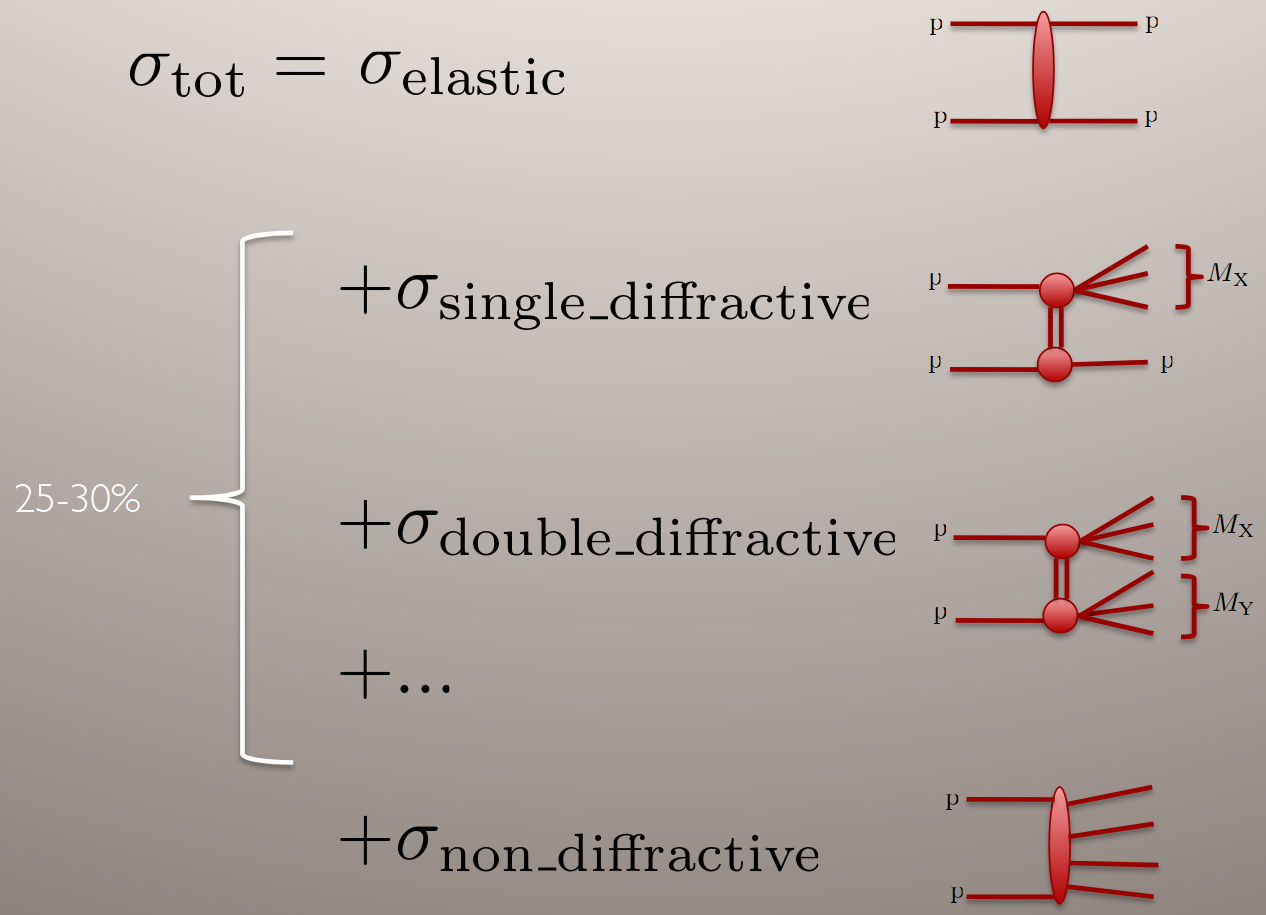
\includegraphics[height=6cm,keepaspectratio]{pics/cross_sections_LHC}};
        \node[below=of diffr,yshift=9mm] {Cross section contribution at LHC energies};
     \end{tikzpicture}
\end{frame}

%------------------------------------------------ 

\section{Central exclusive production at ALICE} %
\begin{frame}
    \frametitle{Diffraction definition}
    Diffractive events are reactions where \textbf{no quantum numbers are exchanged}~$\to$ leads to special topology\\
    \vspace*{5mm}
    \centering\begin{tikzpicture}
        \node[inner sep=0pt] (diffr) at (0,0)
            {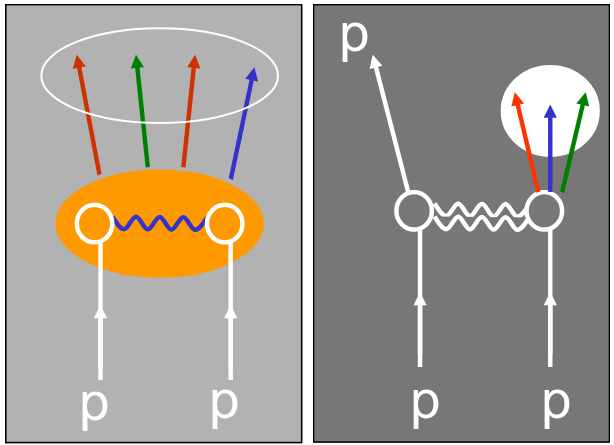
\includegraphics[height=4cm,keepaspectratio]{pics/diffraction_wo}};
        \node (nonD) at (-4.2,0) [text width=3cm] {\small Incident hadrons aquire color\\ $\to$~break apart};
        \node (D) at (4.5,0) [text width=3cm] {\small Colorless exchange};
        \node (nonDbelow) at (-2.5,-3.2) [text width=6cm] {\small$\eta$~gap exponentially supressed};
        \node (Dbelow) at (4.4,-3.2) [text width=6cm] {\small$\eta$~ gap not supressed};
        \node [below=of diffr,yshift=9mm] (eta) [text width=3cm] {\small $\eta=-ln(tan(\frac{\theta}{2}))$};
        % \draw[->] (-3,-2.6) to [out=90,in=270] (-1.5,-2.1) ;
        % \draw[->] (3,-2.6) to [out=90,in=270] (1.5,-2.1) ;
        \draw[->] (-3,-2.8) to [out=90,in=225] (diffr.south west) ;
        \draw[->] (3.3,-2.8) to [out=90,in=315] (diffr.south east) ;
      \end{tikzpicture}
\end{frame}

%------------------------------------------------ 

\begin{frame}
    \frametitle{Rapidity gap}
    \centering\begin{tikzpicture}
        \node[inner sep=0pt] (diffr) at (0,0)
            {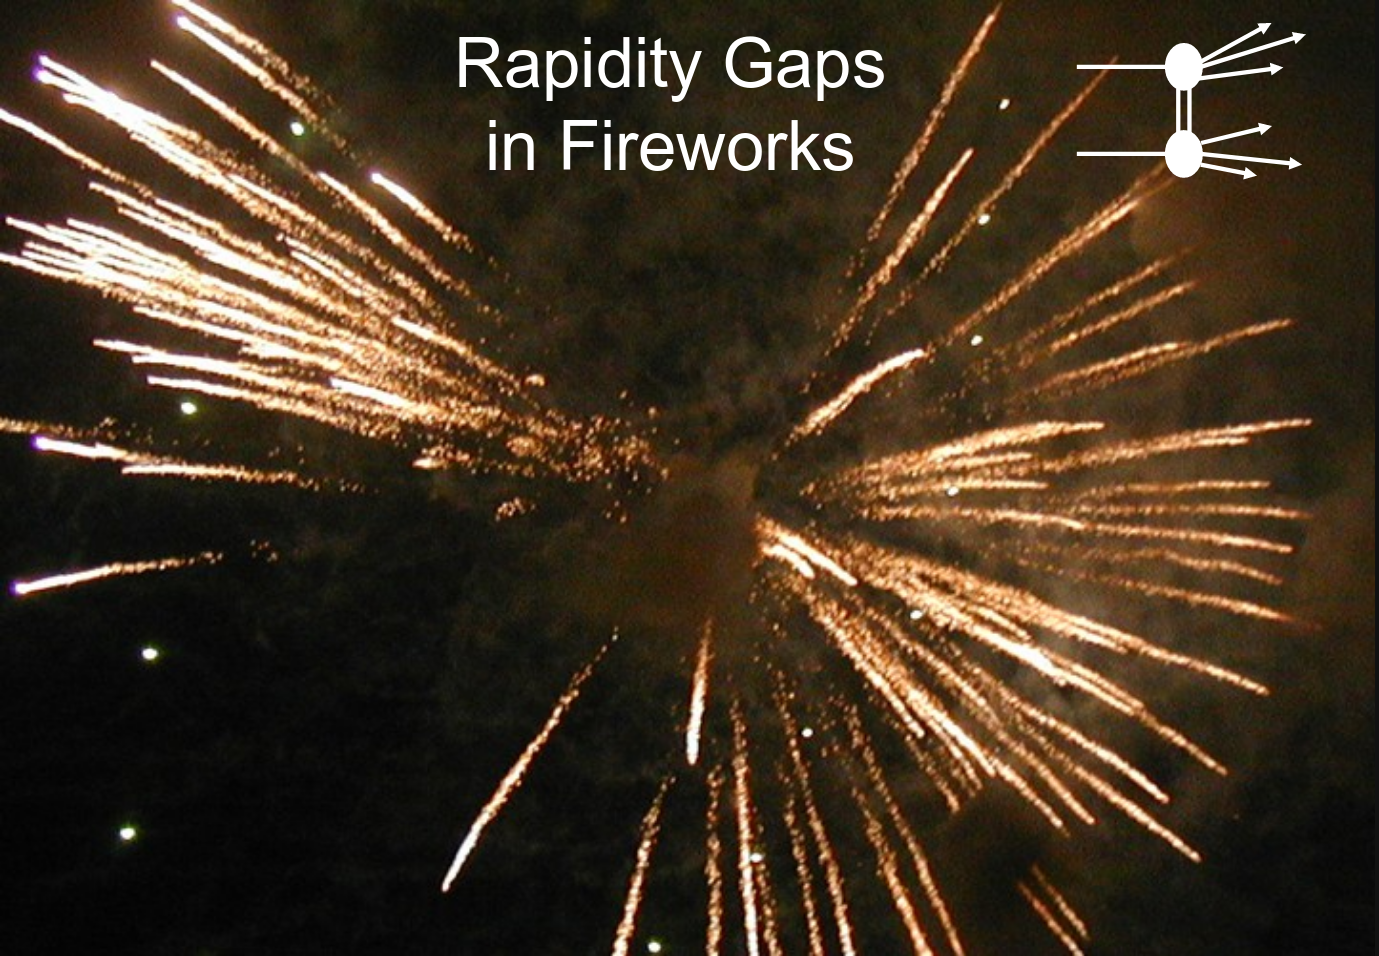
\includegraphics[width=0.8\paperwidth,keepaspectratio]{pics/rapidity_gap}};
     \end{tikzpicture}
\end{frame}

%------------------------------------------------ 

\begin{frame}
    \frametitle{Diffractive processes}
    Different types of diffractive events are distinguished\\
    \vspace*{5mm}
    \centering\begin{tikzpicture}
        \node[inner sep=0pt] (sd) at (-3.5,0) {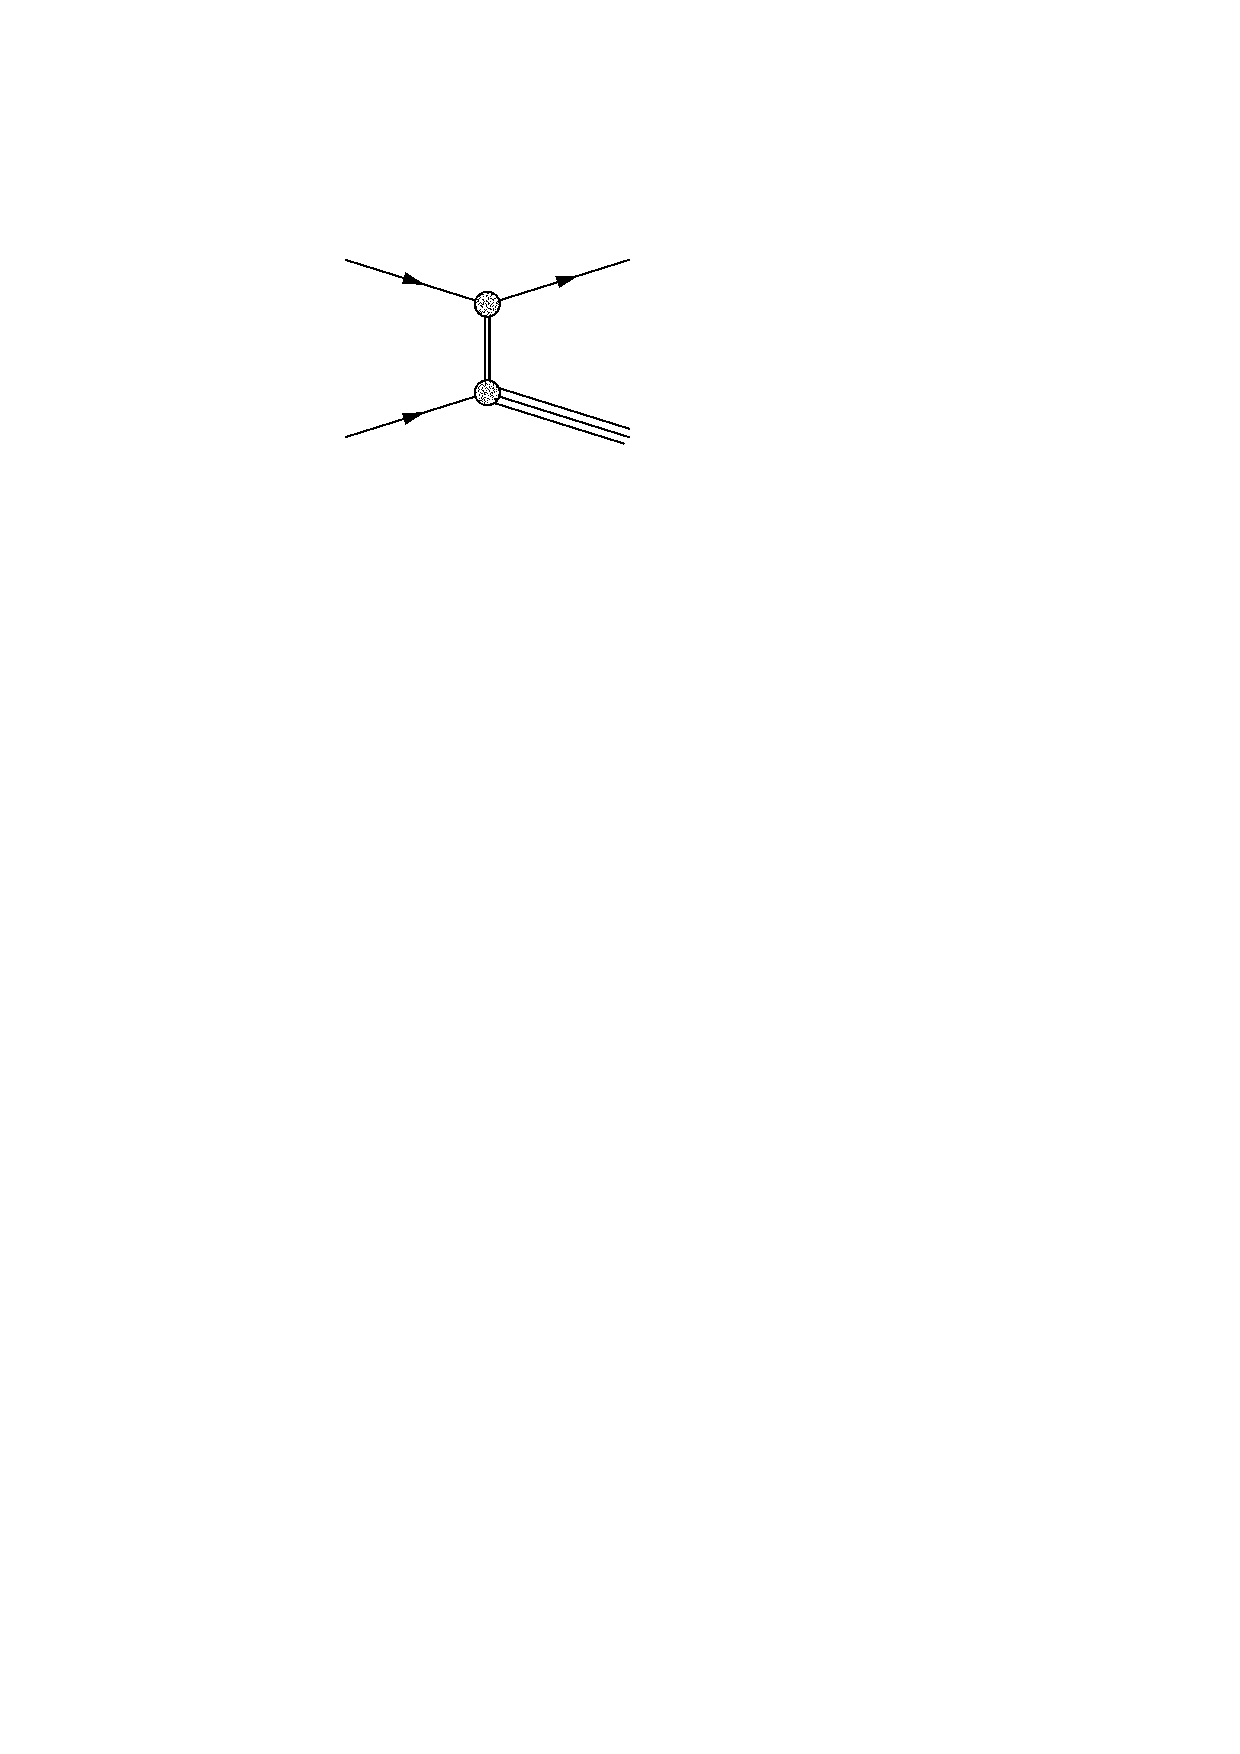
\includegraphics[height=3cm,keepaspectratio]{pics/SD1.pdf}};
        \node[inner sep=0pt] (dd) at (0,0) {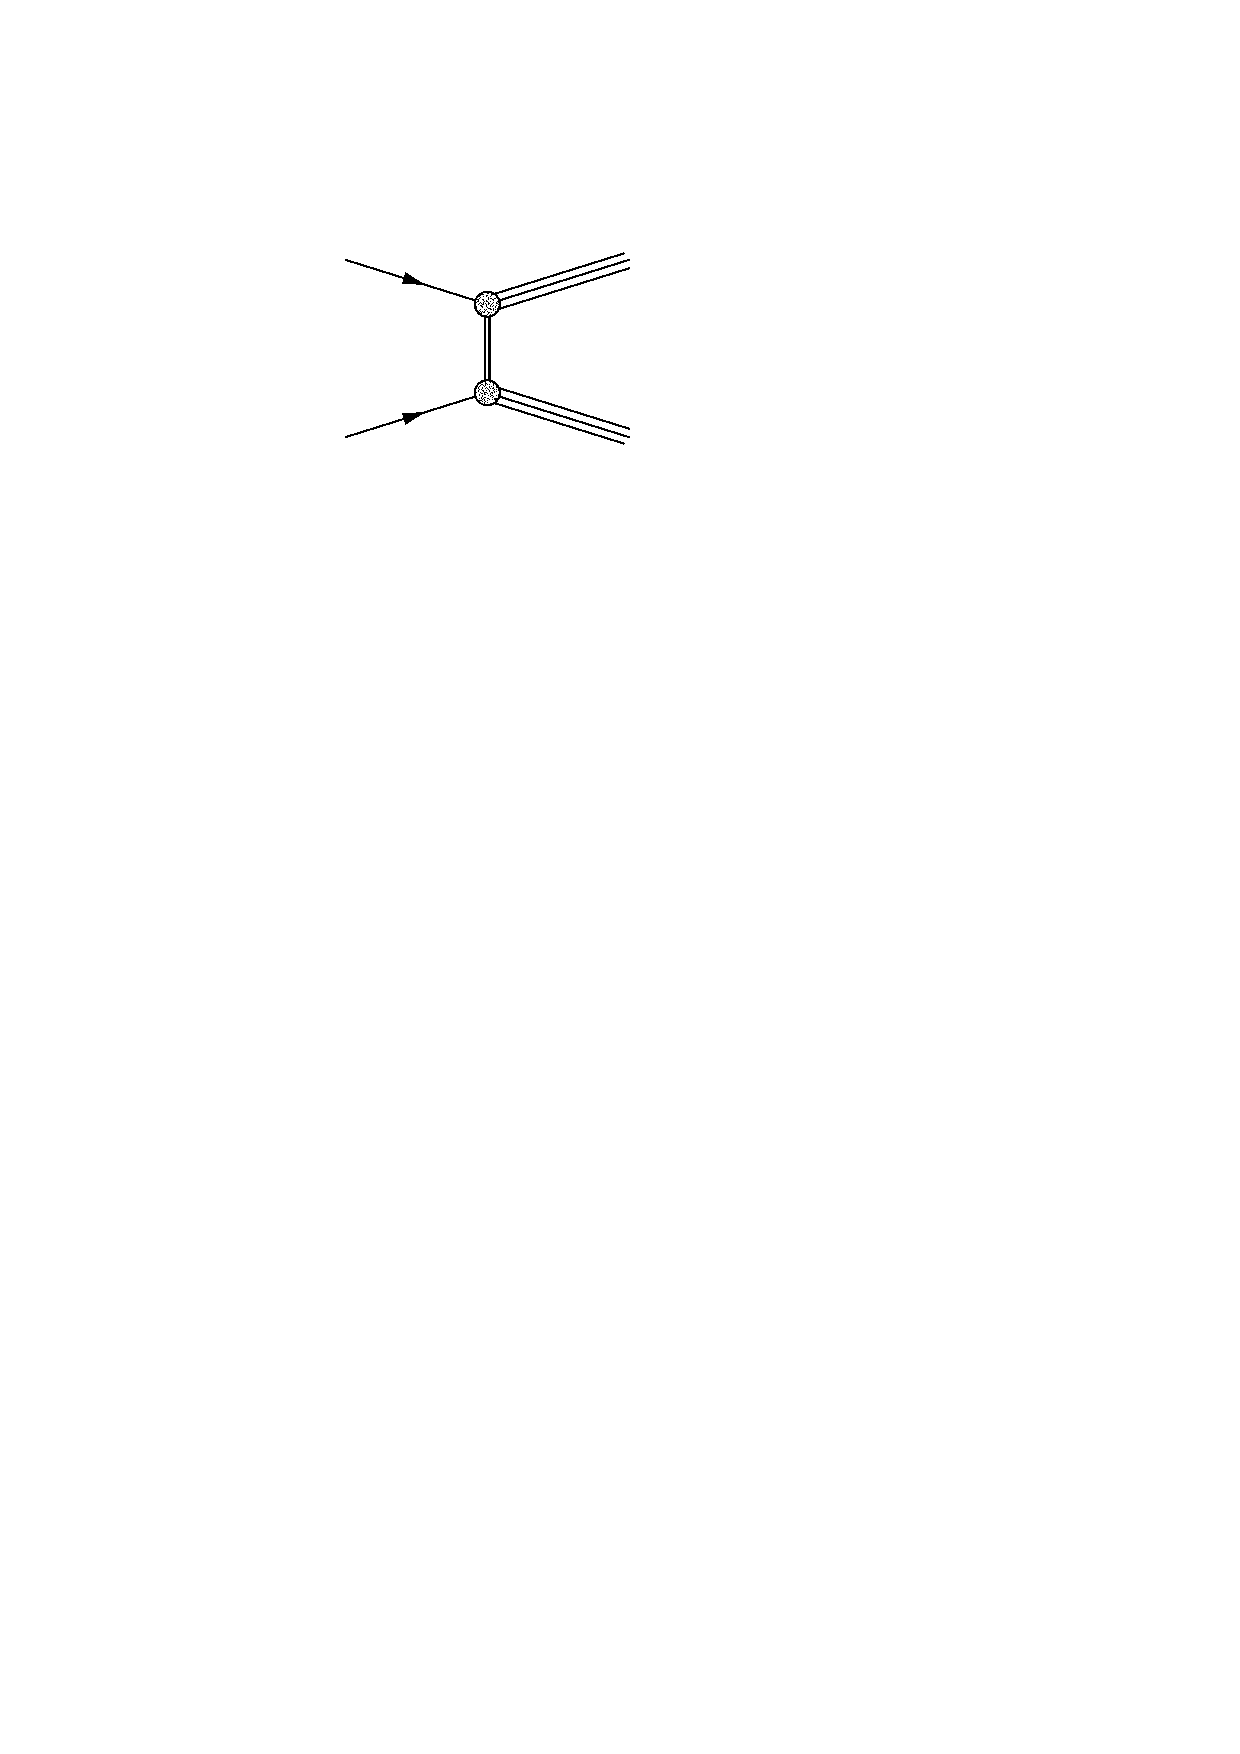
\includegraphics[height=3cm,keepaspectratio]{pics/DD1.pdf}};
        \node[inner sep=0pt] (cep) at (3.5,0) {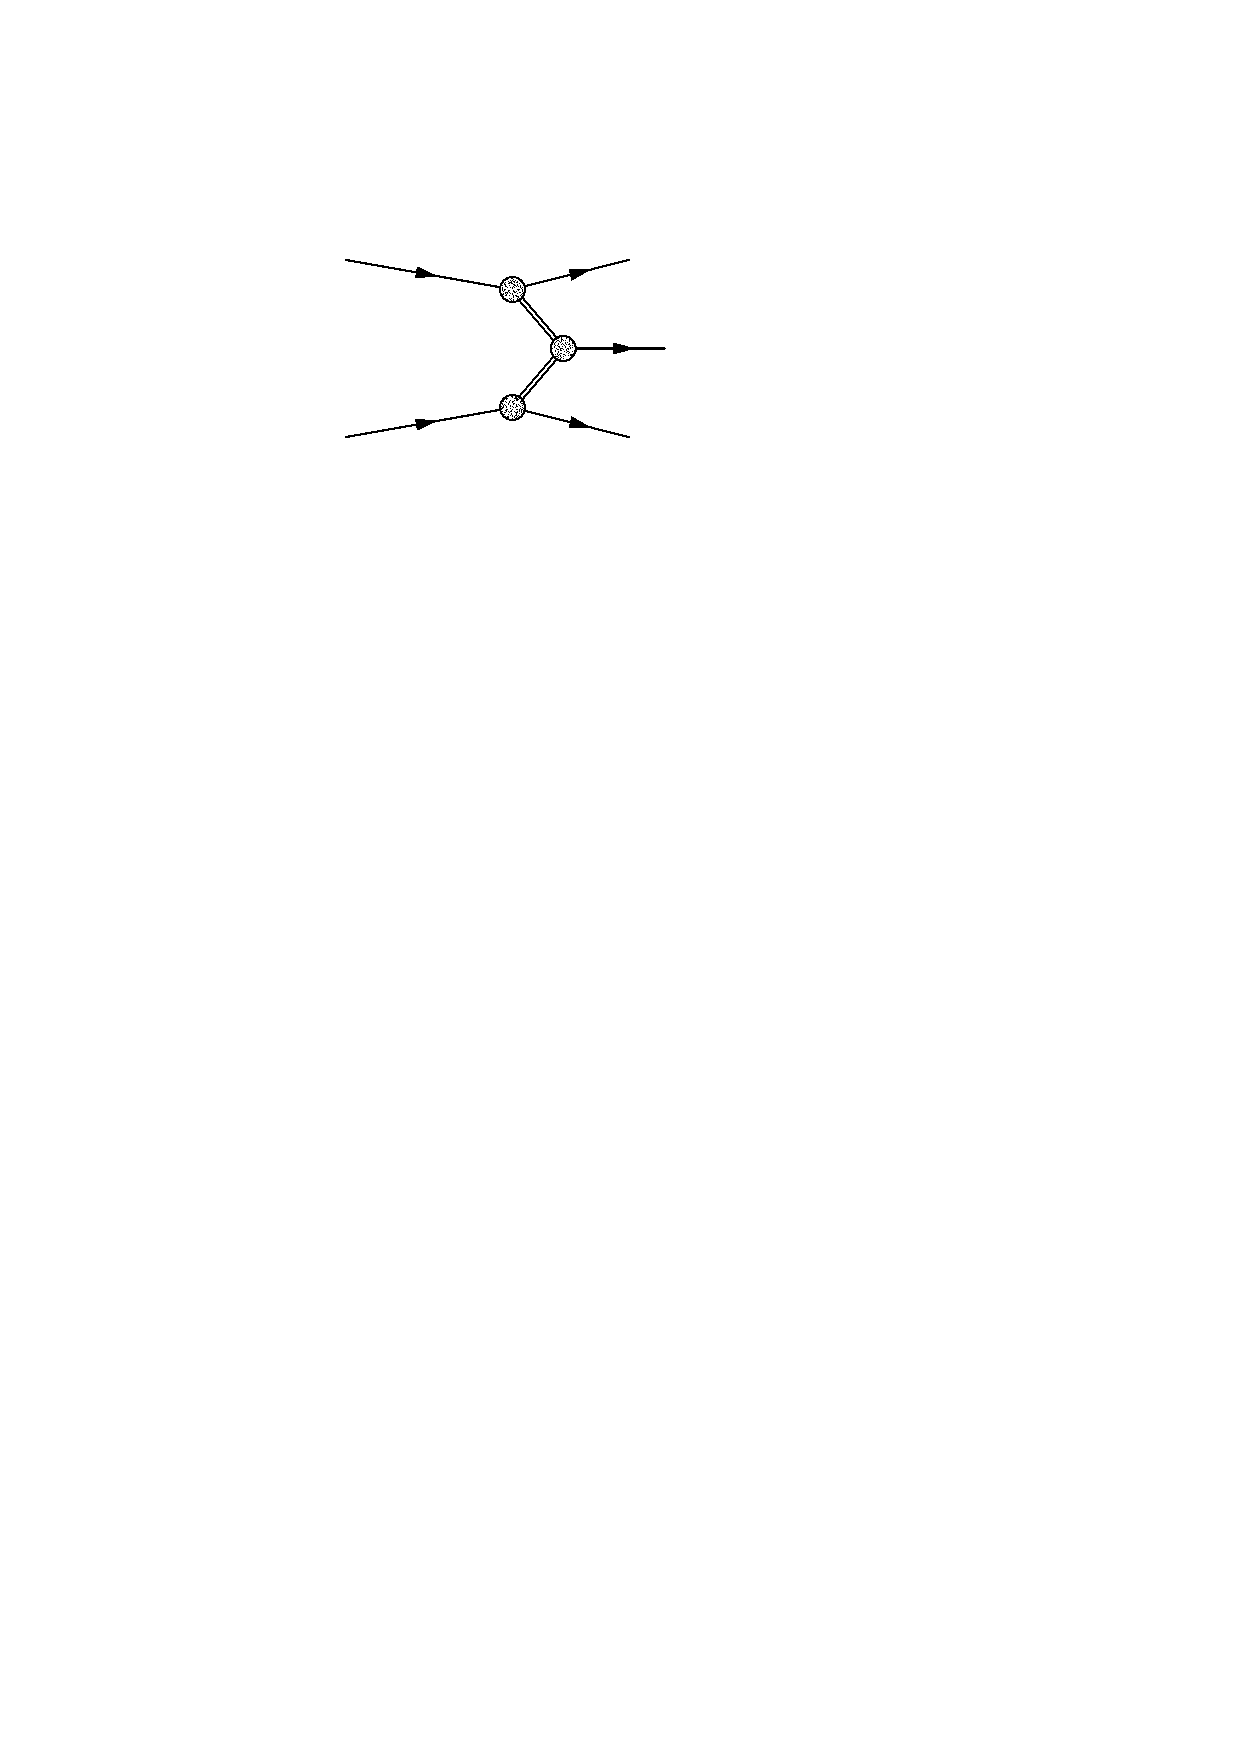
\includegraphics[height=3cm,keepaspectratio]{pics/CEP1.pdf}};
        \node[align = center, below = of sd, yshift=15mm] {\small Single diffractive};
        \node[align = center, below = of dd, yshift=15mm] {\small Double diffractive};
        \node[align = center, below = of cep, yshift=15mm] {\small CEP};
        \node[align = center, below = of cep, xshift=15mm,yshift=30mm] {\small \emph{X}};

        \draw [decorate,decoration={brace,mirror,amplitude=15pt},xshift=0pt,yshift=0pt]
            (-4,-2) -- (4,-2) node [black,midway,yshift=-1.0cm] 
            {Described by \emph{Regge} theory};
 
    \end{tikzpicture}
    
\end{frame}

%------------------------------------------------ 
% \begin{frame}
%     \frametitle{Regge theory - short overview}
%     \begin{itemize}
%         \item<1-> Pomeron $\mathbb{P}$ represents special Regge trajectory \& is a color singlet state of gluons \& has vacuum quantum numbers
%         \item<2-> Contribution to $\sigma_{tot}$ grows with increasing energy
%         \item<3-> Double Pomeron exchange = production mechanism to study glueballs in the mass region below $2~$MeV
%         \item<4-> Pomeron exchange leads to restriction of quantum numbers of $X$\\\hspace*{4mm}$\to J^{PC}=($even$)^{++}$
%     \end{itemize}
% \end{frame}

%------------------------------------------------ 

\begin{frame}
    \frametitle{Event topology}
    \centering\begin{tikzpicture}
        \node[inner sep=0pt] (sd) at (-3.5,0) {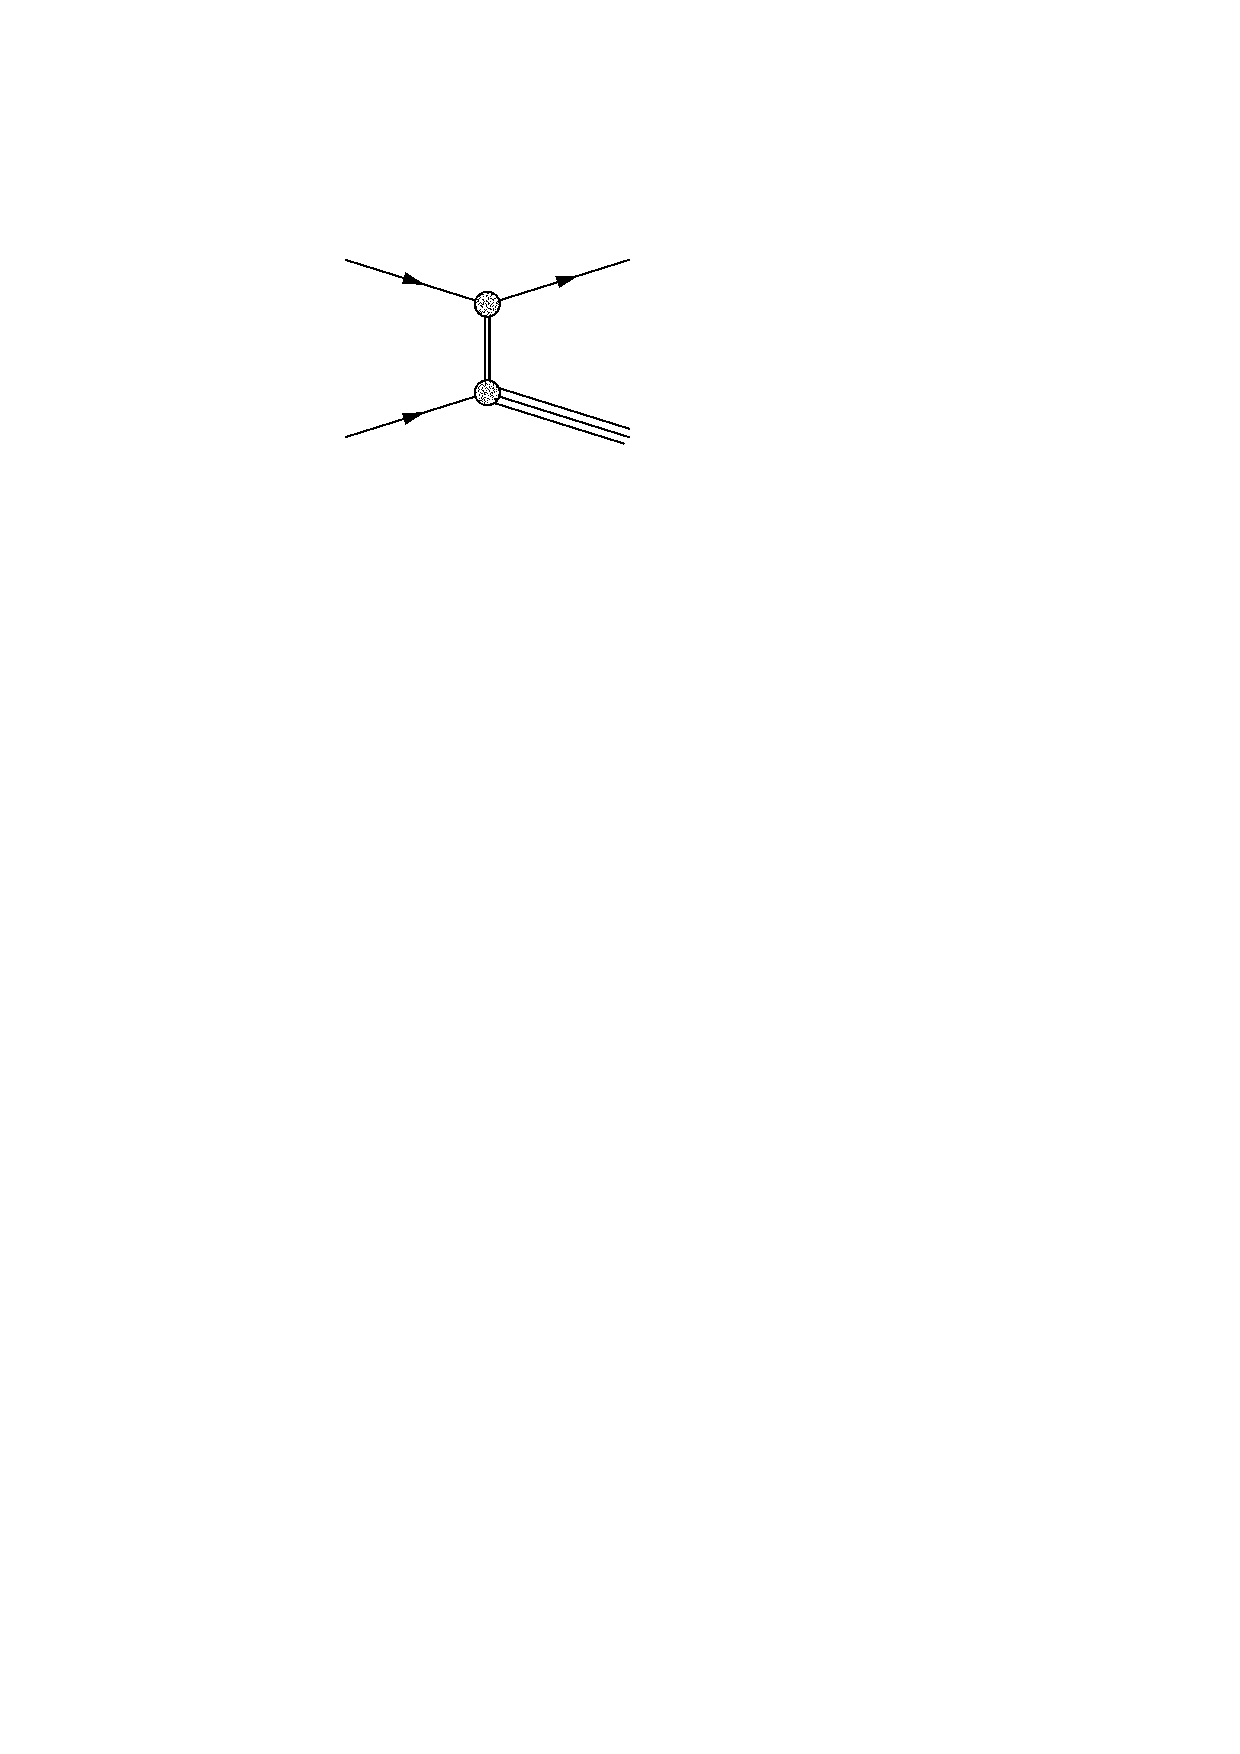
\includegraphics[height=3cm,keepaspectratio]{pics/SD1.pdf}};
        \node[inner sep=0pt] (dd) at (0,0) {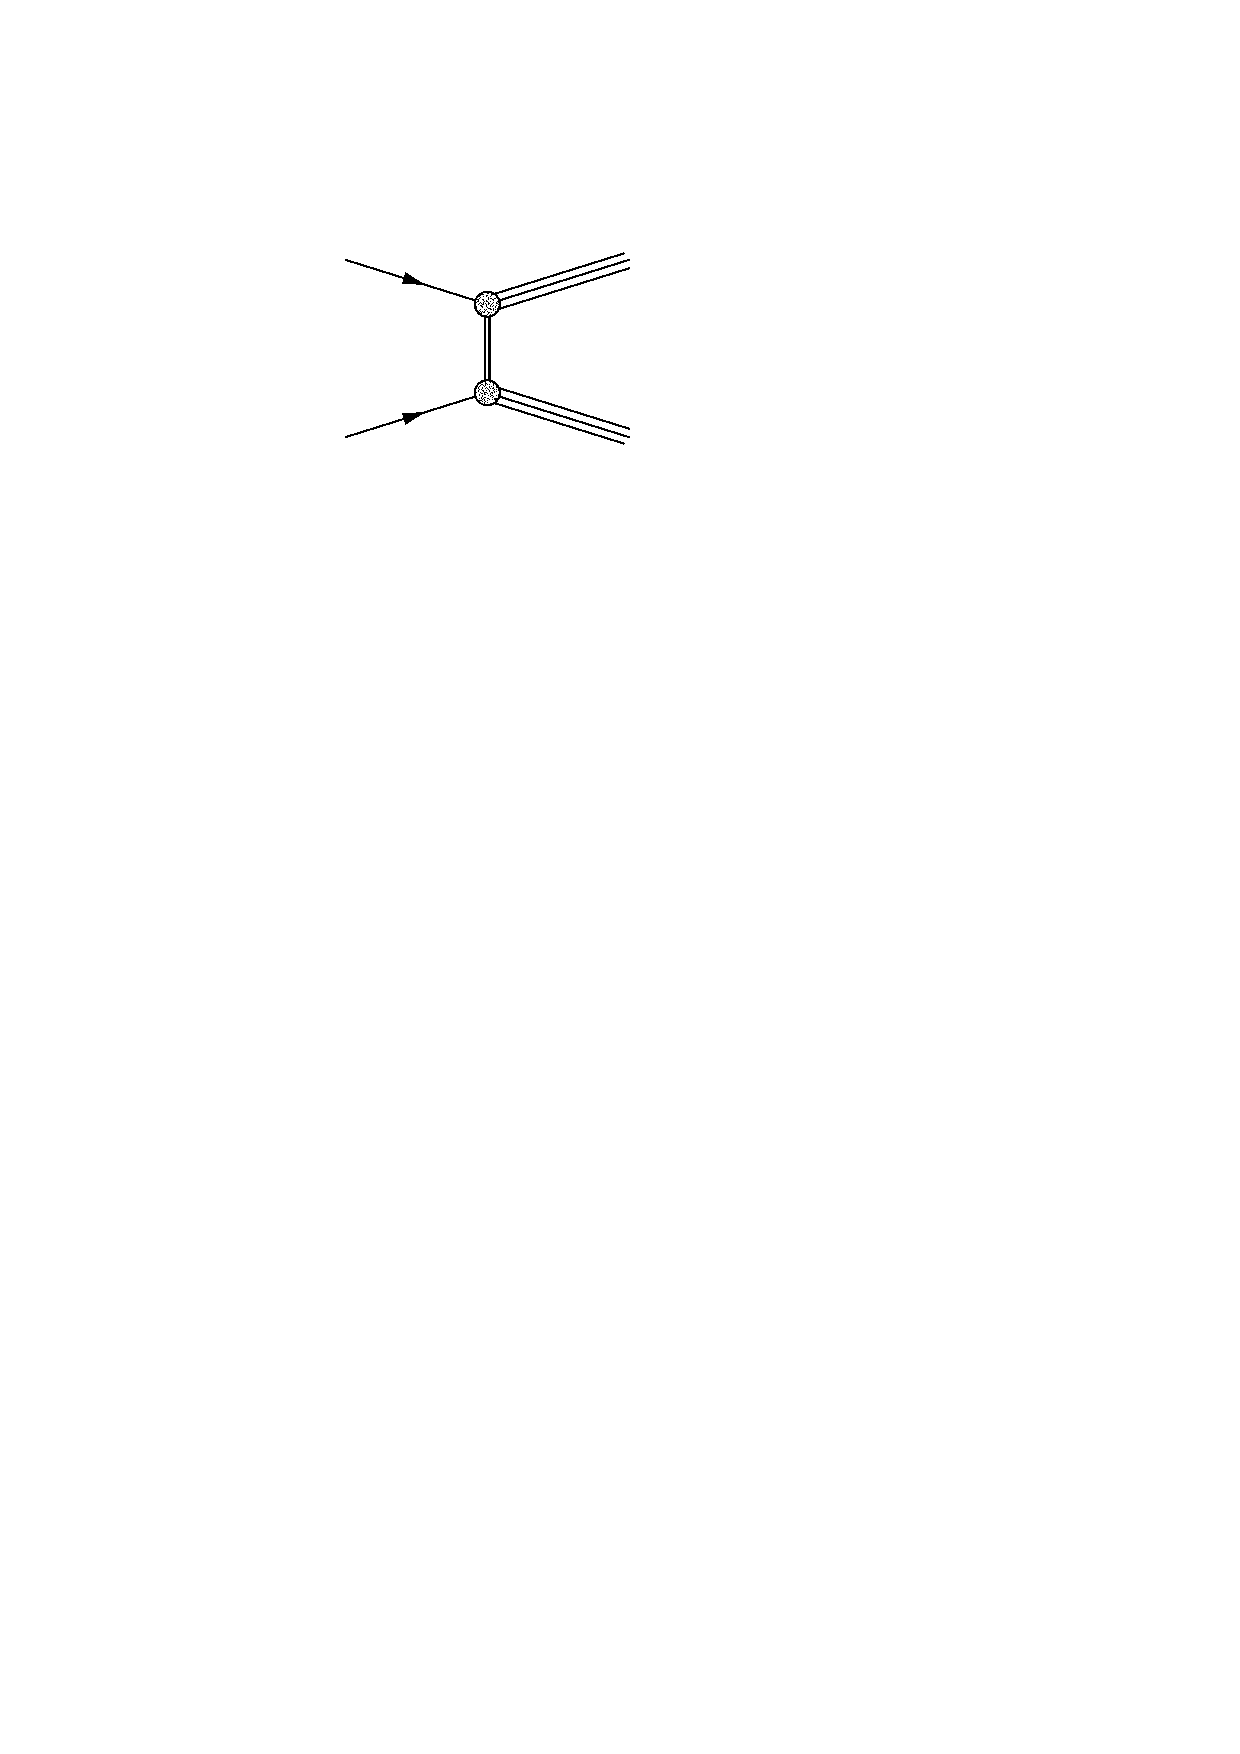
\includegraphics[height=3cm,keepaspectratio]{pics/DD1.pdf}};
        \node[inner sep=0pt] (cep) at (3.5,0) {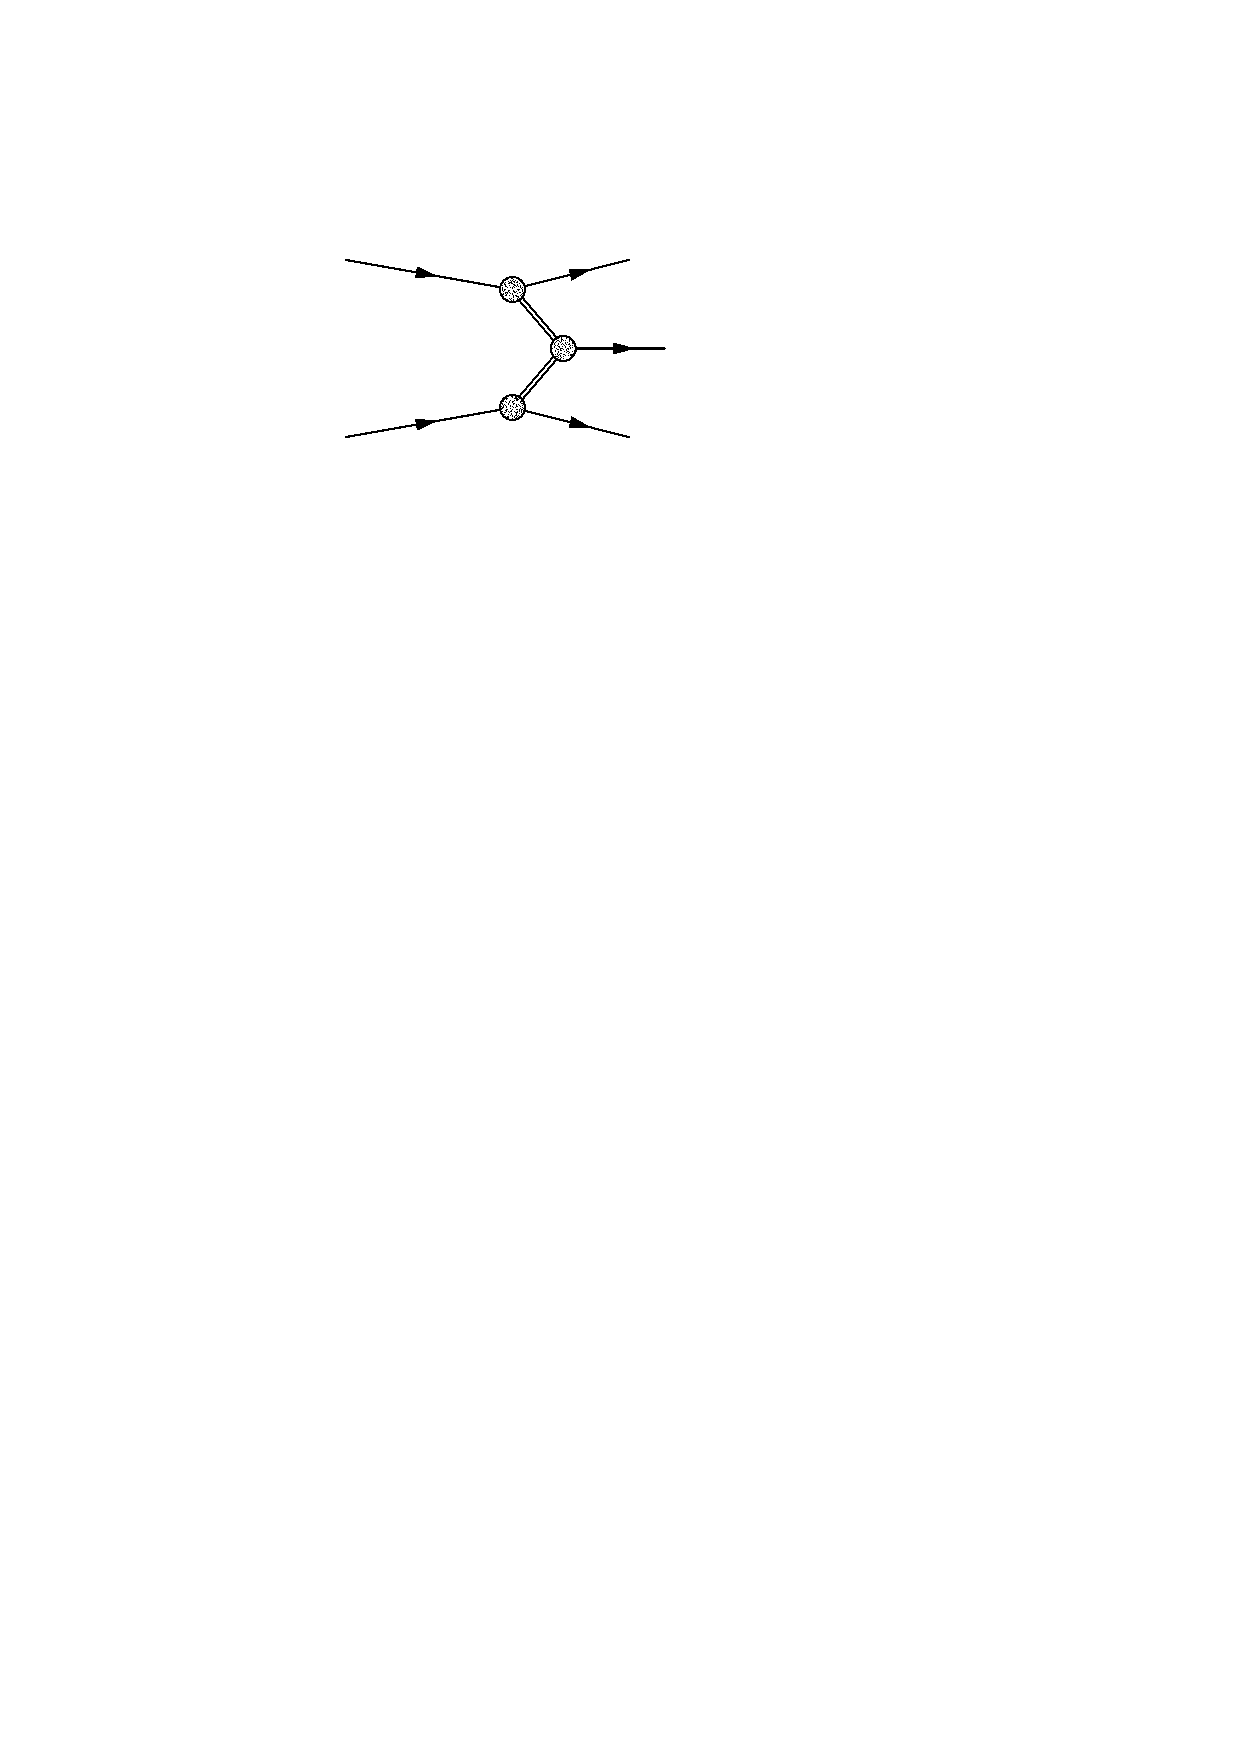
\includegraphics[height=3cm,keepaspectratio]{pics/CEP1.pdf}};
        \node[align = center, above = of sd, yshift=-15mm] {\small Single diffractive};
        \node[align = center, above = of dd, yshift=-15mm] {\small Double diffractive};
        \node[align = center, above = of cep, yshift=-15mm] {\small CEP};
        \node[align = center, below = of cep, xshift=15mm,yshift=30mm] {\small \emph{X}};
 
        \node[inner sep=0pt] (sdtop) at (-3.5,-2.5) {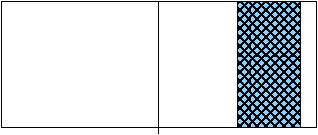
\includegraphics[height=1.1cm,keepaspectratio]{pics/SD_eta}};
        \node[inner sep=0pt] (ddtop) at (0,-2.5) {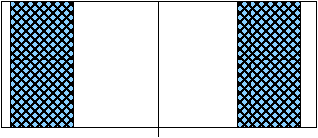
\includegraphics[height=1.1cm,keepaspectratio]{pics/DD_eta}};
        \node[inner sep=0pt] (ceptop) at (3.5,-2.5) {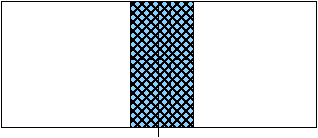
\includegraphics[height=1.1cm,keepaspectratio]{pics/CEP_eta}};
        \node[below=of sdtop, node distance=0cm, yshift=10mm, xshift=11mm] {\small$\eta$};
        \node[left=of sdtop, node distance=0cm, rotate=0, anchor=center,yshift=4mm, xshift=8mm] {\small$\phi$};
        \node[below=of ddtop, node distance=0cm, yshift=10mm, xshift=11mm] {\small$\eta$};
        \node[left=of ddtop, node distance=0cm, rotate=0, anchor=center,yshift=4mm, xshift=8mm] {\small$\phi$};
        \node[below=of ceptop, node distance=0cm, yshift=10mm, xshift=11mm] {\small$\eta$};
        \node[left=of ceptop, node distance=0cm, rotate=0, anchor=center,yshift=4mm, xshift=8mm] {\small$\phi$};

    \end{tikzpicture}
\end{frame}

%------------------------------------------------ 

\begin{frame}
    \frametitle{Event topology}
    \centering\begin{tikzpicture}
        \node[inner sep=0pt] (sdtop) at (-3.5,0) {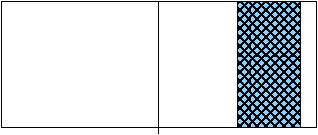
\includegraphics[height=1.1cm,keepaspectratio]{pics/SD_eta}};
        \node[inner sep=0pt] (ddtop) at (0,0) {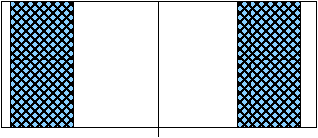
\includegraphics[height=1.1cm,keepaspectratio]{pics/DD_eta}};
        \node[inner sep=0pt] (ceptop) at (3.5,0) {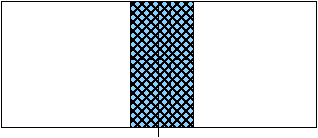
\includegraphics[height=1.1cm,keepaspectratio]{pics/CEP_eta}};

        \node[align = center, above = of sdtop, yshift=-9mm] {\small Single diffractive};
        \node[align = center, above = of ddtop, yshift=-9mm] {\small Double diffractive};
        \node[align = center, above = of ceptop, yshift=-9mm] {\small CEP};

        \node[below=of sdtop, node distance=0cm, yshift=10mm, xshift=11mm] {\small$\eta$};
        \node[left=of sdtop, node distance=0cm, rotate=0, anchor=center,yshift=4mm, xshift=8mm] {\small$\phi$};
        \node[below=of ddtop, node distance=0cm, yshift=10mm, xshift=11mm] {\small$\eta$};
        \node[left=of ddtop, node distance=0cm, rotate=0, anchor=center,yshift=4mm, xshift=8mm] {\small$\phi$};
        \node[below=of ceptop, node distance=0cm, yshift=10mm, xshift=11mm] {\small$\eta$};
        \node[left=of ceptop, node distance=0cm, rotate=0, anchor=center,yshift=4mm, xshift=8mm] {\small$\phi$};

        \draw [decorate,decoration={brace,mirror,amplitude=15pt},xshift=0pt,yshift=0pt]
            (-4,-1) -- (4,-1) node [black,midway,yshift=-1.0cm] 
            {Large $eta$~gap compared to non-diffractive event};

        \node[inner sep=0pt] (nd) at (0,-4) {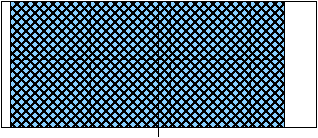
\includegraphics[height=1.1cm,keepaspectratio]{pics/ND_eta}};
        \node[align = center, above = of nd, yshift=-9mm] {\small Non-diffractive};
        \node[below=of nd, node distance=0cm, yshift=10mm, xshift=11mm] {\small$\eta$};
        \node[left=of nd, node distance=0cm, rotate=0, anchor=center,yshift=4mm, xshift=8mm] {\small$\phi$};
    \end{tikzpicture}
\end{frame}

%------------------------------------------------ 

\begin{frame}
    \frametitle{Event selection}
    Large rapidity gaps in \emph{non-diffractive} events are exponentially supressed
    \centering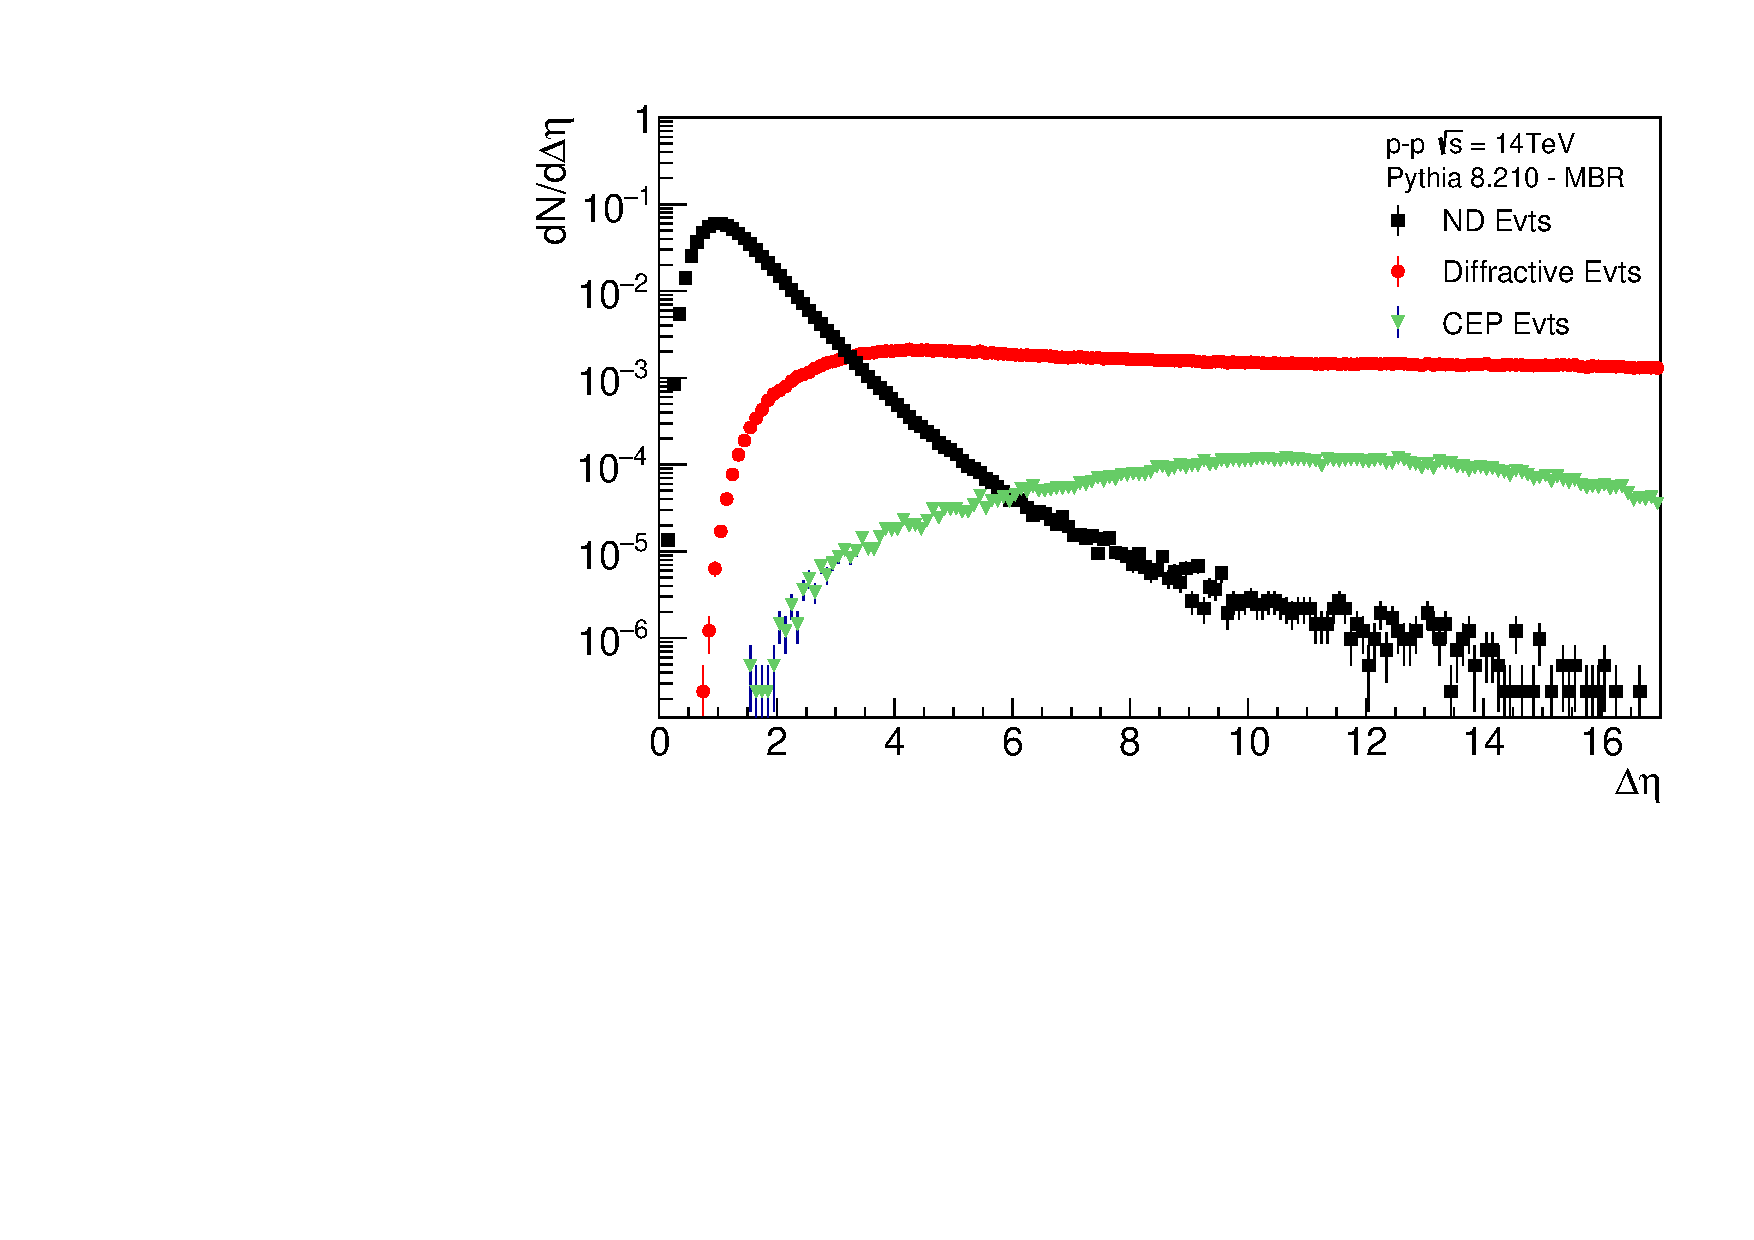
\includegraphics[height=6cm,keepaspectratio]{pics/newDeltaEta_biggerSymbols.pdf}
\end{frame}

%------------------------------------------------ 

\begin{frame}
    \frametitle{The ALICE detector system}
    \centering\begin{tikzpicture}
        \node[inner sep=0pt] (det) at (-3.3,0) {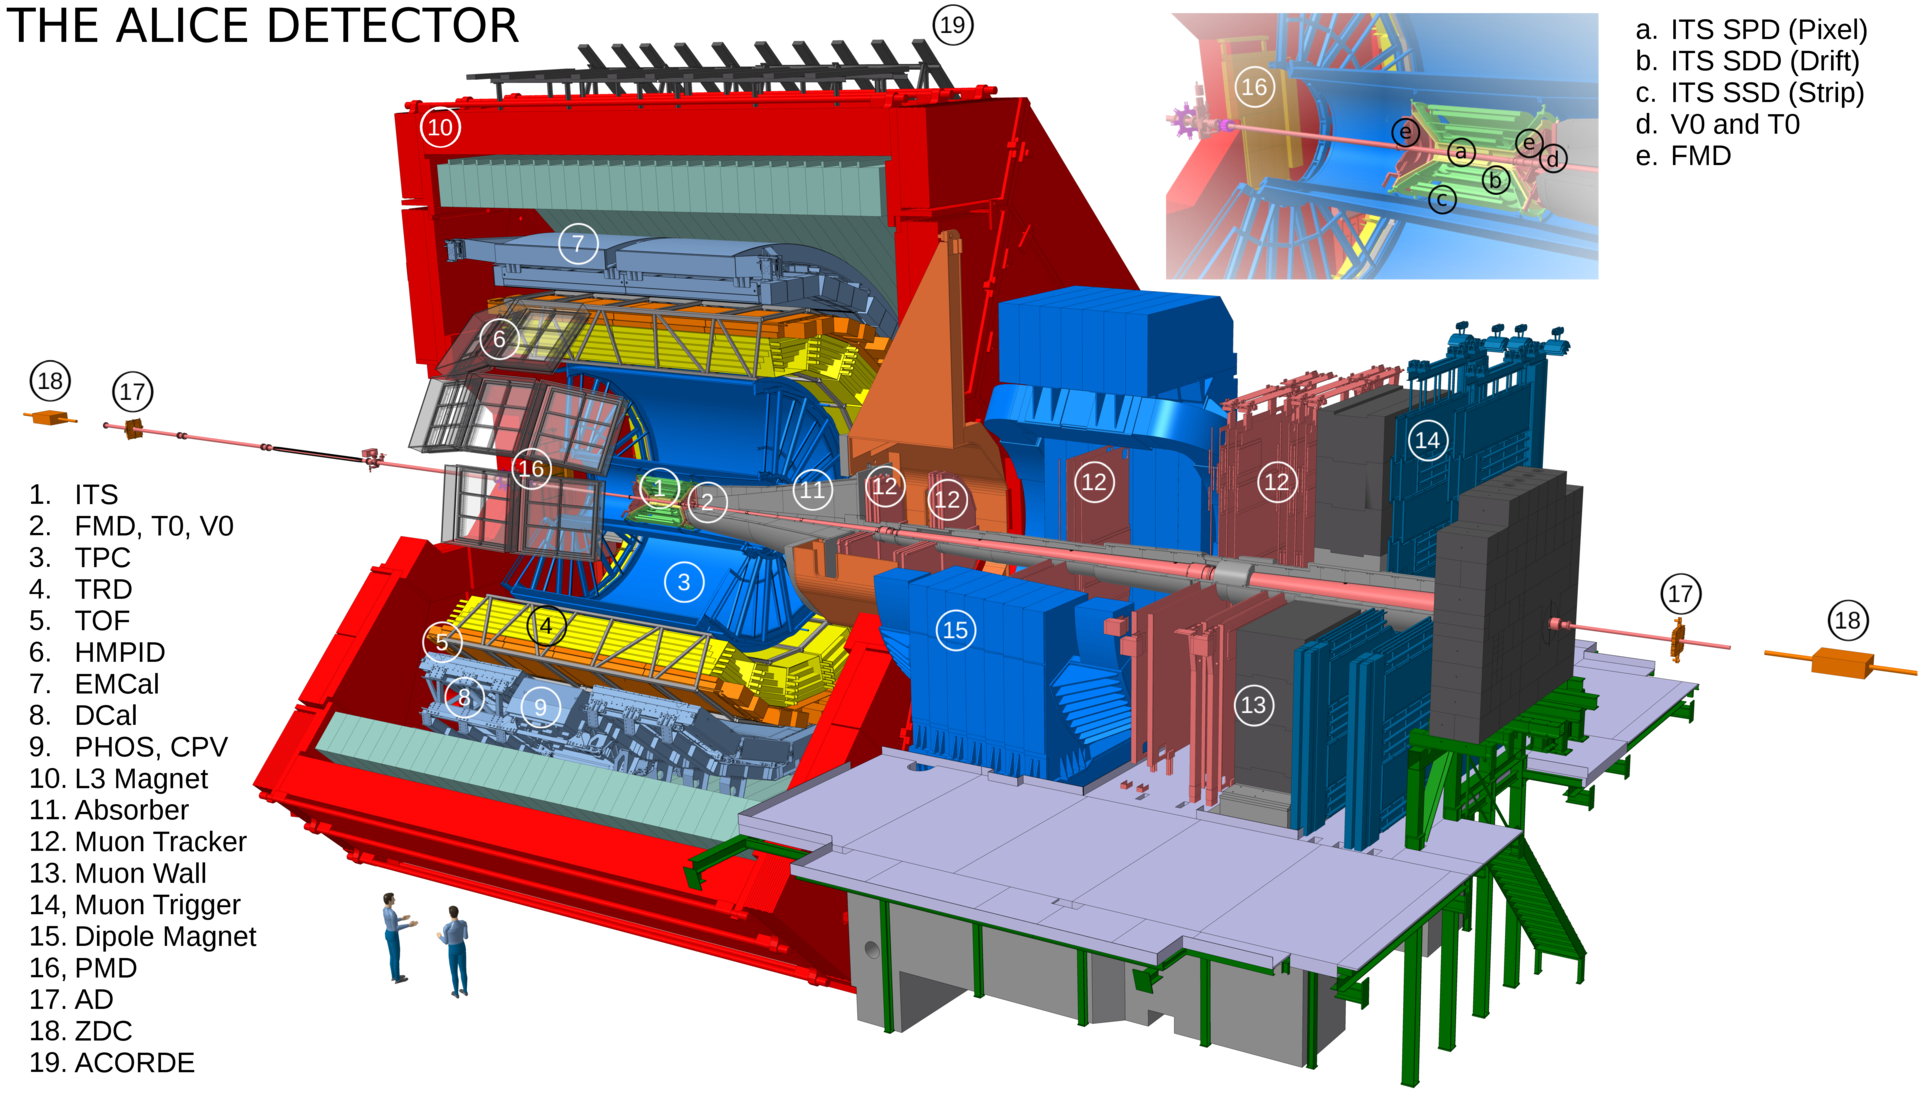
\includegraphics[height=3.3cm,keepaspectratio]{pics/2017-May-11-ALICE_RUN2_labels_HD}};
        \node[inner sep=0pt] (cov) at (3.3,0) {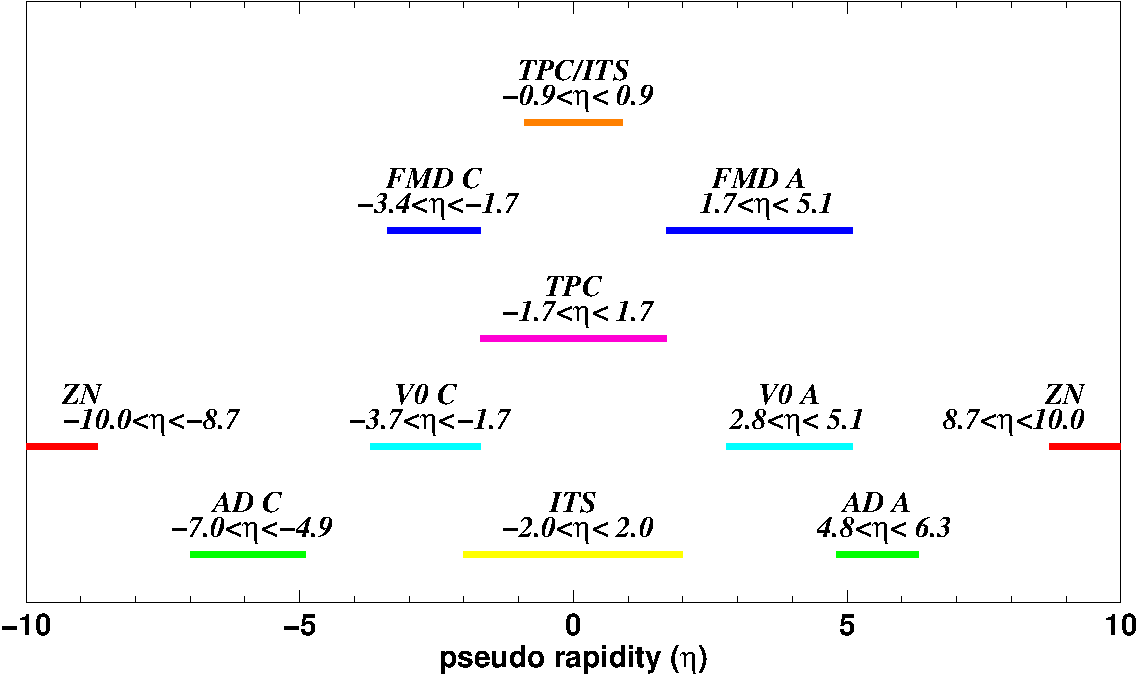
\includegraphics[height=3.3cm,keepaspectratio]{pics/ALICE_eta_coverage}};
        \draw[->, thick] (det) -- (cov);

        \node[align = center, above = of det, yshift=-9mm] {\small ALICE detector};
        \node[align = center, above = of cov, yshift=-9mm] {\small $\eta$ coverage};

        \node<2>[] (centralbarrel) at (0,-3) {\small Central barrel $\to$ determine $p^{\mu}$};
        \node<2> (rectbarrel) at (3.35,0.18) [rectangle, dashed, minimum height=28mm,minimum width=8mm,draw, thick] {};
        \draw<2>[->, ultra thick] (centralbarrel) -- (-4.0,-0.0);
        \draw<2>[->, ultra thick] (centralbarrel) -- (rectbarrel);

        \node<3->[] (vetodets) at (0,-3) {\small Small detectors for global event characterisation};
        \node<3-> (rectbarrel1) at (4.6,0.18) [rectangle, dashed, minimum height=28mm,minimum width=16mm,draw, thick] {};
        \node<3-> (rectbarrel2) at (2.1,0.18) [rectangle, dashed, minimum height=28mm,minimum width=16mm,draw, thick] {};
        \draw<3->[->, ultra thick] (vetodets) -- (rectbarrel1);
        \draw<3->[->, ultra thick] (vetodets) -- (rectbarrel2);

        % \node (rectroot) at (0,0) [rectangle, dashed, color=red, minimum height=2cm,minimum width=3cm,draw, thick] {};
        % \node (rootbottom) [below=1mm of rectroot, color=red]  {Root node};
 
        % \node[inner sep=0pt] (nd) at (0,-4) {\[includegraphicsheight=1.1cm,keepaspectratio]{pics/ND_eta}};
        % \node[align = center, below = of nd, yshift=9mm] {\small Non-diffractive};
        % \node[below=of nd, node distance=0cm, yshift=10mm, xshift=11mm] {\small$\eta$};
        % \node[left=of nd, node distance=0cm, rotate=0, anchor=center,yshift=4mm, xshift=8mm] {\small$\phi$};
    \end{tikzpicture}
        
    % \centering\includegraphics[height=6cm,keepaspectratio]{pics/}
\end{frame}

%------------------------------------------------ 

\begin{frame}
    \frametitle{Central exclusive production at ALICE}
    To study the CEP events a $\eta$ gap condition is used
    \begin{enumerate}
        \item<2-> Signal in the central barrel
        \item<3-> No activity in veto detectors
    \end{enumerate}
    
    \vspace*{2mm}
    \centering\begin{tikzpicture}
        \node[inner sep=0pt] (cov) at (3.3,0) {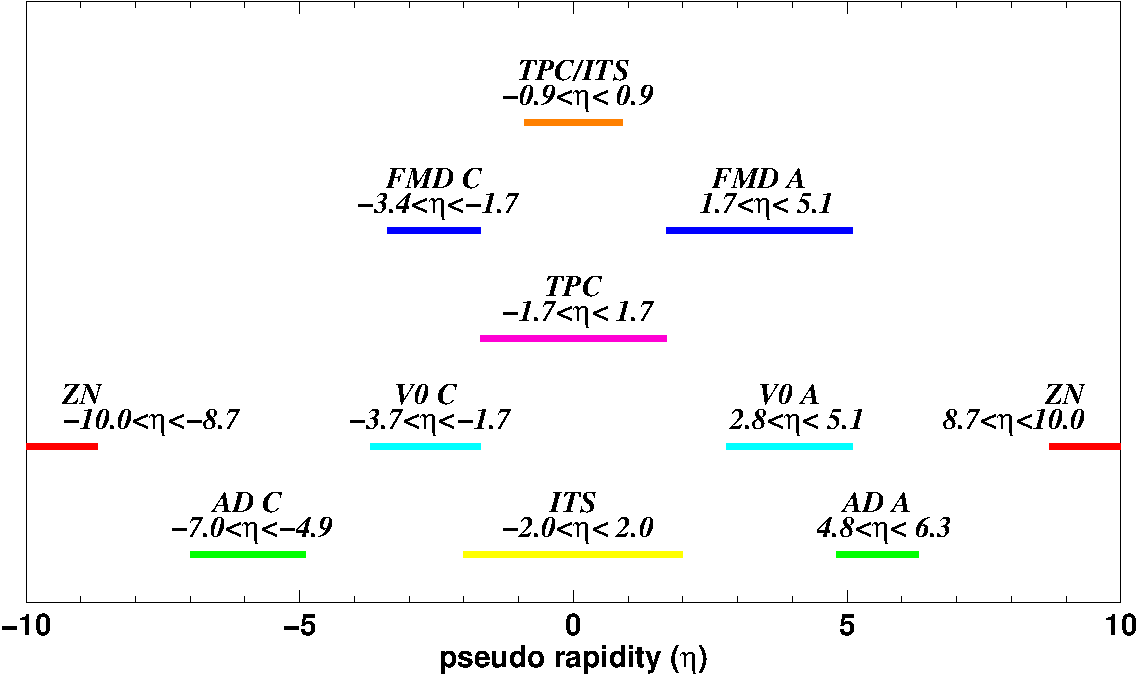
\includegraphics[height=3.3cm,keepaspectratio]{pics/ALICE_eta_coverage}};
        \node[inner sep=0pt] (det) at (-3.3,0) {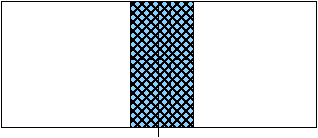
\includegraphics[height=2.5cm,keepaspectratio]{pics/CEP_eta}};
        \draw[->, thick] (det) -- (cov);
        % \node[below=of det, node distance=0cm, yshift=10mm, xshift=11mm] {\small$\eta$};
        % \node[left=of det, node distance=0cm, rotate=0, anchor=center,yshift=4mm, xshift=8mm] {\small$\phi$};

        \node[align = center, above = of det, yshift=-9mm] {\small CEP event};
        \node[align = center, above = of cov, yshift=-9mm] {\small $\eta$ coverage};

        \node<2-> (rectbarrel) at (3.35,0.18) [color=red,rectangle, dashed, minimum height=28mm,minimum width=8mm,draw, thick] {};

        \node<3-> (rectbarrel1) at (4.6,0.18) [rectangle, dashed, minimum height=28mm,minimum width=16mm,draw, thick] {};
        \node<3-> (rectbarrel2) at (2.1,0.18) [rectangle, dashed, minimum height=28mm,minimum width=16mm,draw, thick] {};

        % \node (rectroot) at (0,0) [rectangle, dashed, color=red, minimum height=2cm,minimum width=3cm,draw, thick] {};
        % \node (rootbottom) [below=1mm of rectroot, color=red]  {Root node};
 
        % \node[inner sep=0pt] (nd) at (0,-4) {\[includegraphicsheight=1.1cm,keepaspectratio]{pics/ND_eta}};
        % \node[align = center, below = of nd, yshift=9mm] {\small Non-diffractive};
        % \node[below=of nd, node distance=0cm, yshift=10mm, xshift=11mm] {\small$\eta$};
        % \node[left=of nd, node distance=0cm, rotate=0, anchor=center,yshift=4mm, xshift=8mm] {\small$\phi$};
    \end{tikzpicture}
        
    % \centering\includegraphics[height=6cm,keepaspectratio]{pics/}
\end{frame}

%------------------------------------------------ 

\begin{frame}
    \frametitle{Regge theory - short overview}
    \begin{itemize}
        \item<1-> Reactions characterized by a color neutral \emph{t}~-channel exchange carrying vacuum quantum numbers\\$\to$ Quantum number filter on $J^{PC} = (\text{even})^{++}$~states
        \item<2-> CEP $\to$ hadron spectroscopy for $<2.5$~GeV
        \begin{itemize}
            \item<2-> Study mass spectrum
            \item<3-> Lightest \emph{glueball} predicted in that region $J^{PC} = (0)^{++}$~state
        \end{itemize}
    \end{itemize}
    \centering\begin{tikzpicture}
        \node<2->[inner sep=0pt] (cep) at (0,0) {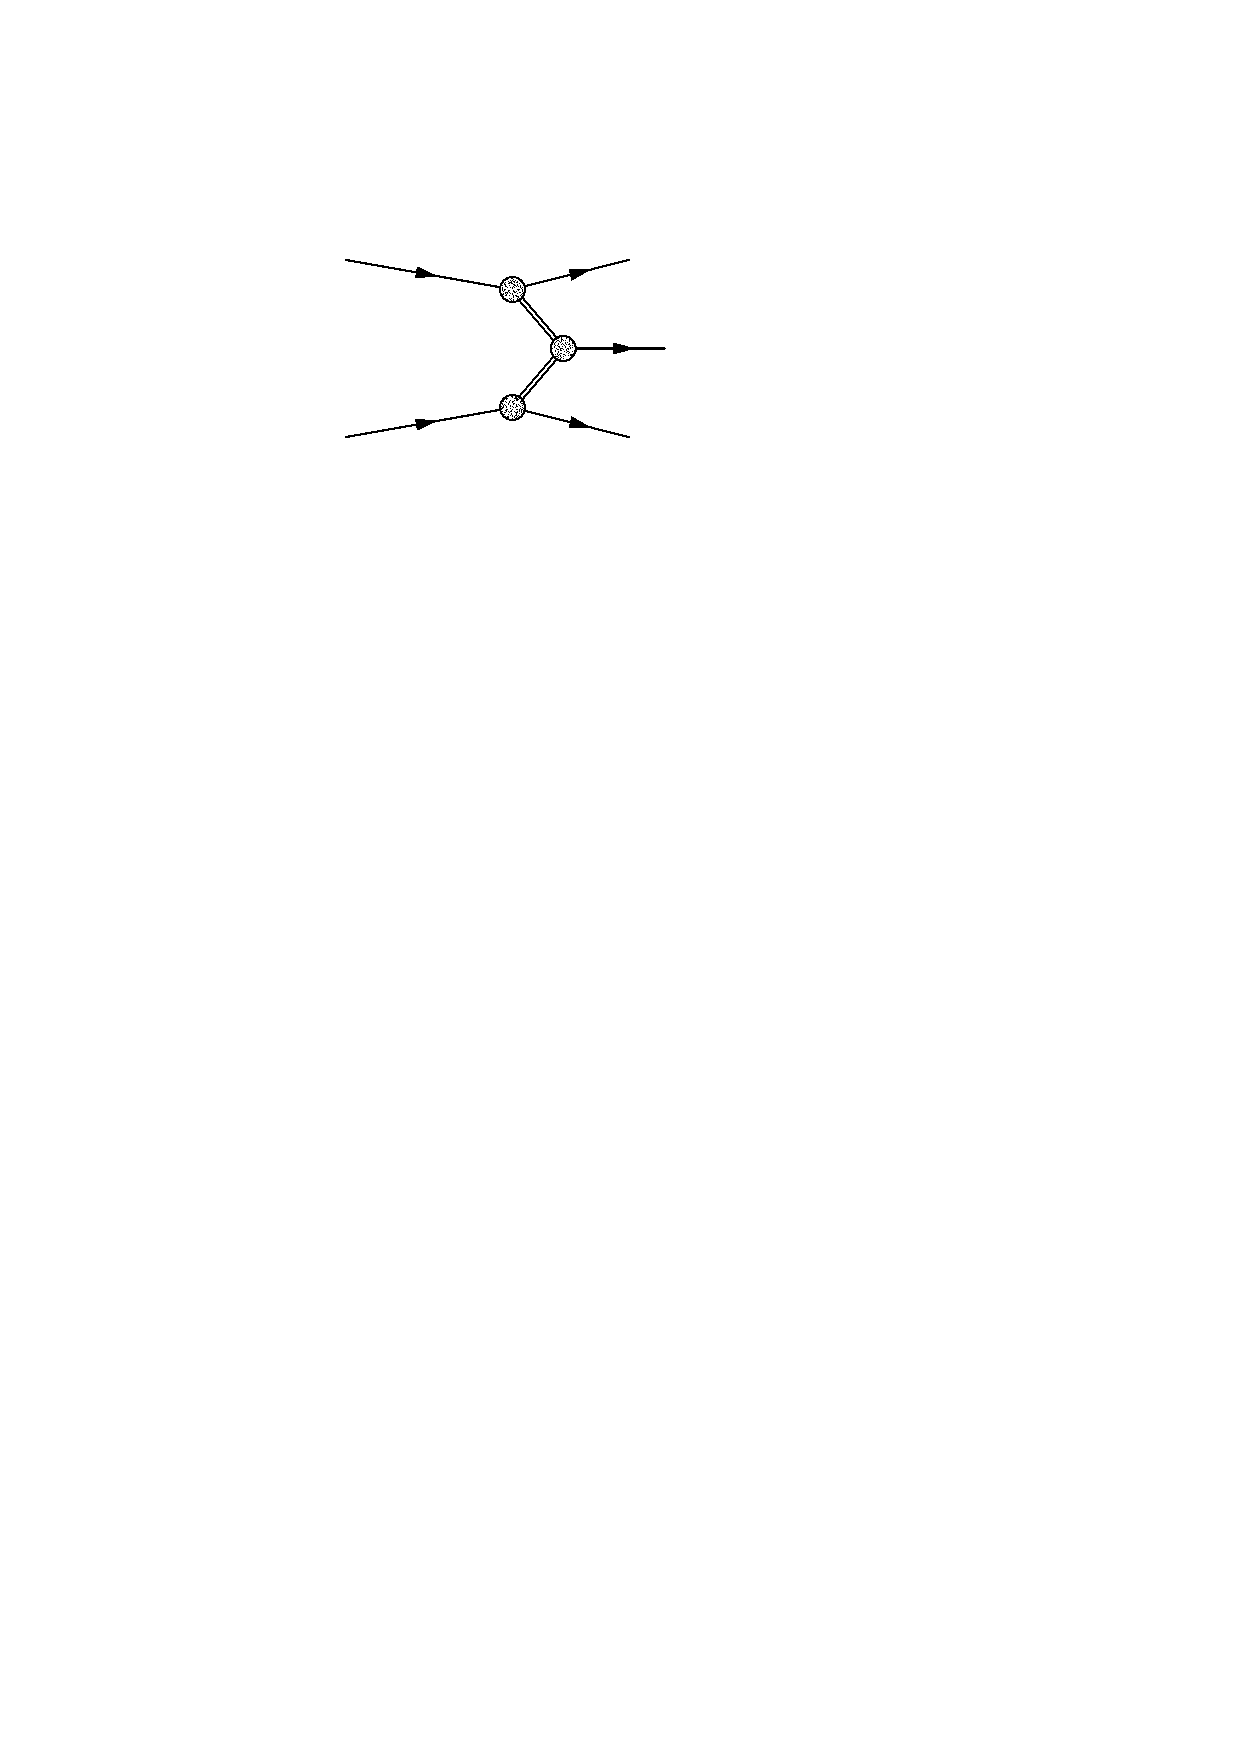
\includegraphics[height=3cm,keepaspectratio]{pics/CEP1.pdf}};
        % \node[align = center, above = of cep, yshift=-15mm] {\small CEP};
        \node[below=of cep, xshift=18mm,yshift=28mm] (X) {\small \emph{X}};
        \node[align = center, right = of X, xshift=0mm,yshift=5mm] (part1) {\small $\pi,K$};
        \node[align = center, right = of X, xshift=0mm,yshift=-5mm] (part2) {\small $\pi,K$};
        \draw[->,thick] (X) -- (part1);
        \draw[->,thick] (X) -- (part2);
    \end{tikzpicture}
 
\end{frame}

%------------------------------------------------ 

\begin{frame}
    \frametitle{Regge theory - short overview}
    \centering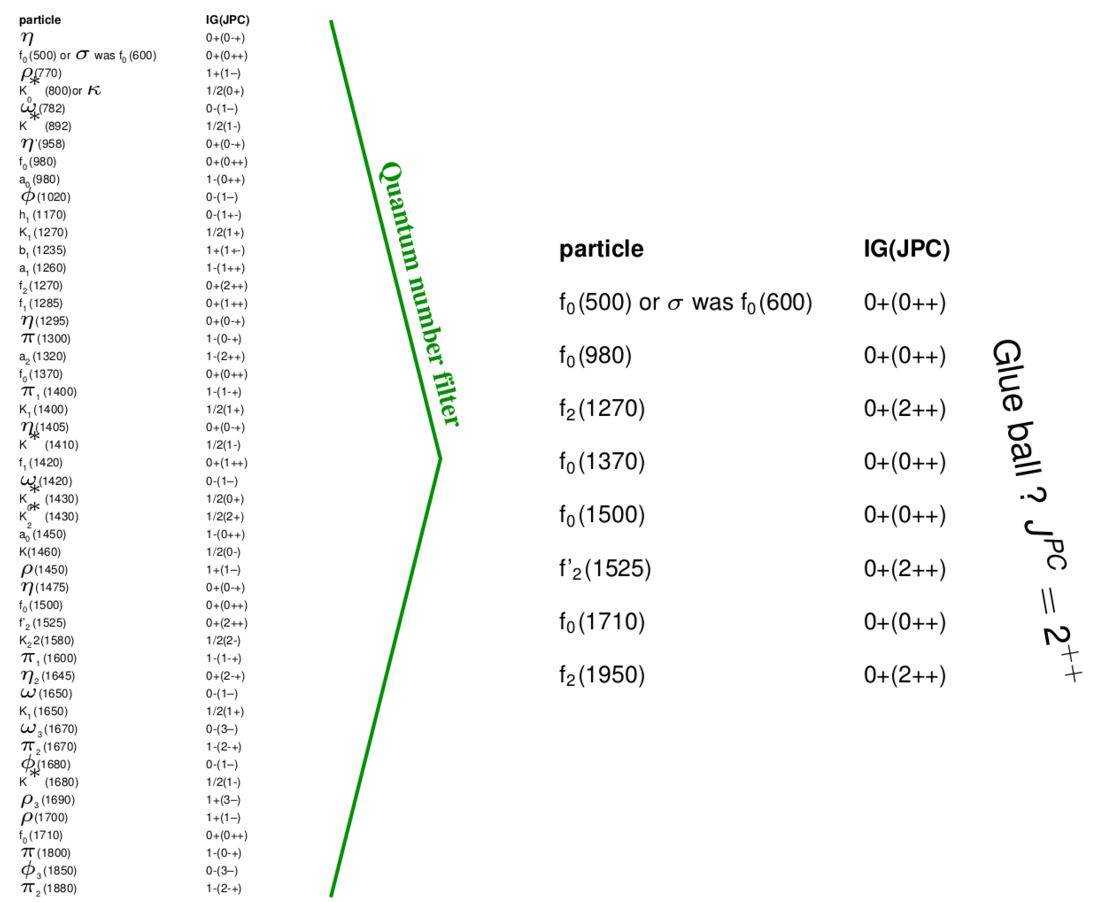
\includegraphics[height=8cm, keepaspectratio]{pics/mesons_mass_range}

\end{frame}

%------------------------------------------------ 

\begin{frame}
    \frametitle{Invariant mass spectrum}
    Studying \emph{Pythia-8} simulations yield
    \begin{itemize}
        \item<1-> Enforcing $\eta$ gap cut reduces non-diffractive almost entirely  
        \item<2-> Remaining background are partially recontructed CEP events - \textbf{feed down}
    \end{itemize}
    % \vspace*{1mm}
    \centering\begin{tikzpicture}
        \node<1-2>[inner sep=0pt] (cov) at (0,0) {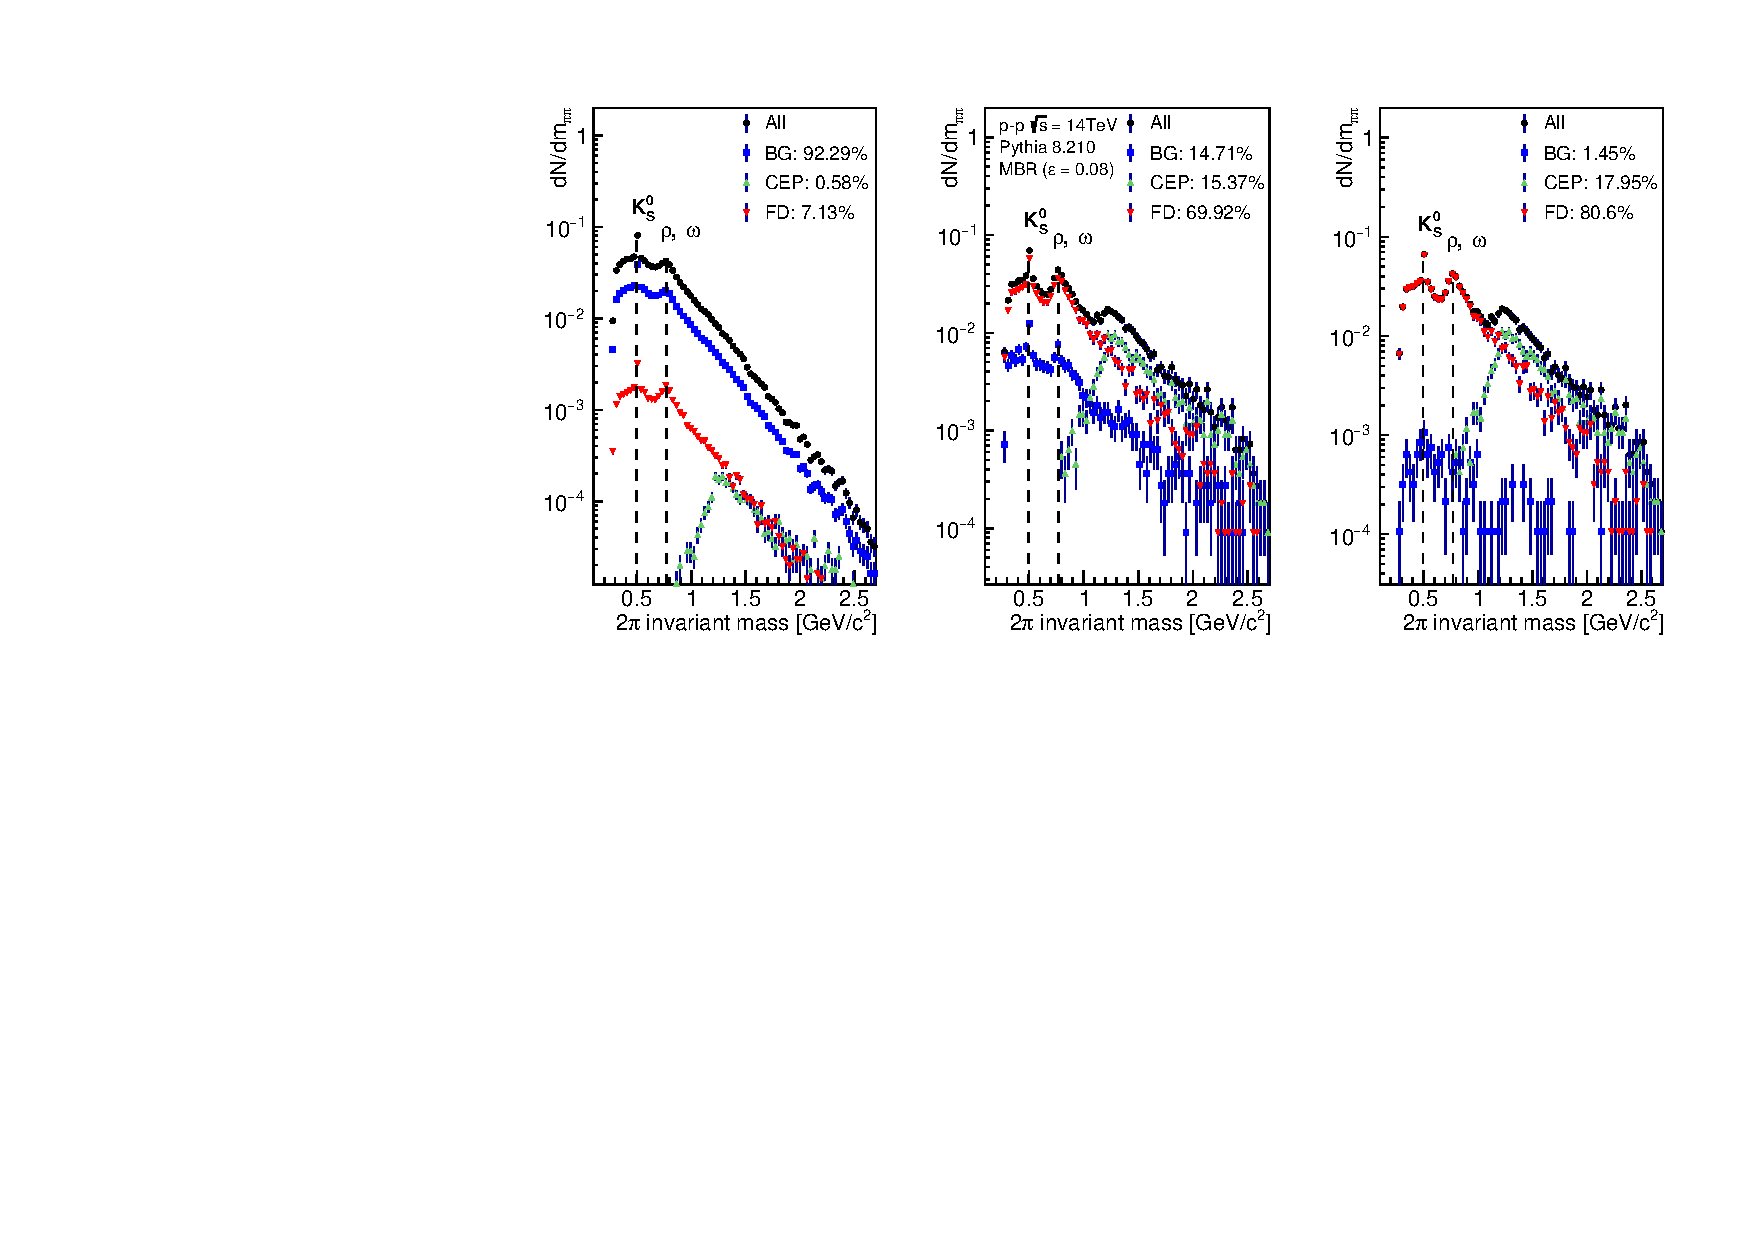
\includegraphics[height=5.1cm,keepaspectratio]{pics/detected_simulated_newLabels}};
        \node[above=of cov, yshift=-15mm] (txt) {$\to$~increasing~$\Delta\eta$};

        % \draw[->, thick] (det) -- (cov);

        % \node[align = center, above = of det, yshift=-9mm] {\small CEP event};
        % \node[align = center, above = of cov, yshift=-9mm] {\small $\eta$ coverage};

        % \node<2-> (rectbarrel) at (3.35,0.18) [color=red,rectangle, dashed, minimum height=28mm,minimum width=8mm,draw, thick] {};

        % \node<3-> (rectbarrel1) at (4.6,0.18) [rectangle, dashed, minimum height=28mm,minimum width=16mm,draw, thick] {};
        % \node<3-> (rectbarrel2) at (2.1,0.18) [rectangle, dashed, minimum height=28mm,minimum width=16mm,draw, thick] {};

        % \node (rectroot) at (0,0) [rectangle, dashed, color=red, minimum height=2cm,minimum width=3cm,draw, thick] {};
        % \node (rootbottom) [below=1mm of rectroot, color=red]  {Root node};

        % \node[inner sep=0pt] (nd) at (0,-4) {\[includegraphicsheight=1.1cm,keepaspectratio]{pics/ND_eta}};
        % \node[align = center, below = of nd, yshift=9mm] {\small Non-diffractive};
        % \node[below=of nd, node distance=0cm, yshift=10mm, xshift=11mm] {\small$\eta$};
        % \node[left=of nd, node distance=0cm, rotate=0, anchor=center,yshift=4mm, xshift=8mm] {\small$\phi$};
    \end{tikzpicture}
 
\end{frame}

%------------------------------------------------ 

\begin{frame}
    \frametitle{Feed down}
    \textbf{Feed down} \emph{vs} \text{fully reconstructed} events\\
    \vspace*{3mm}
    \centering\begin{tikzpicture}
        \node[inner sep=0pt] (cep) at (0,0) {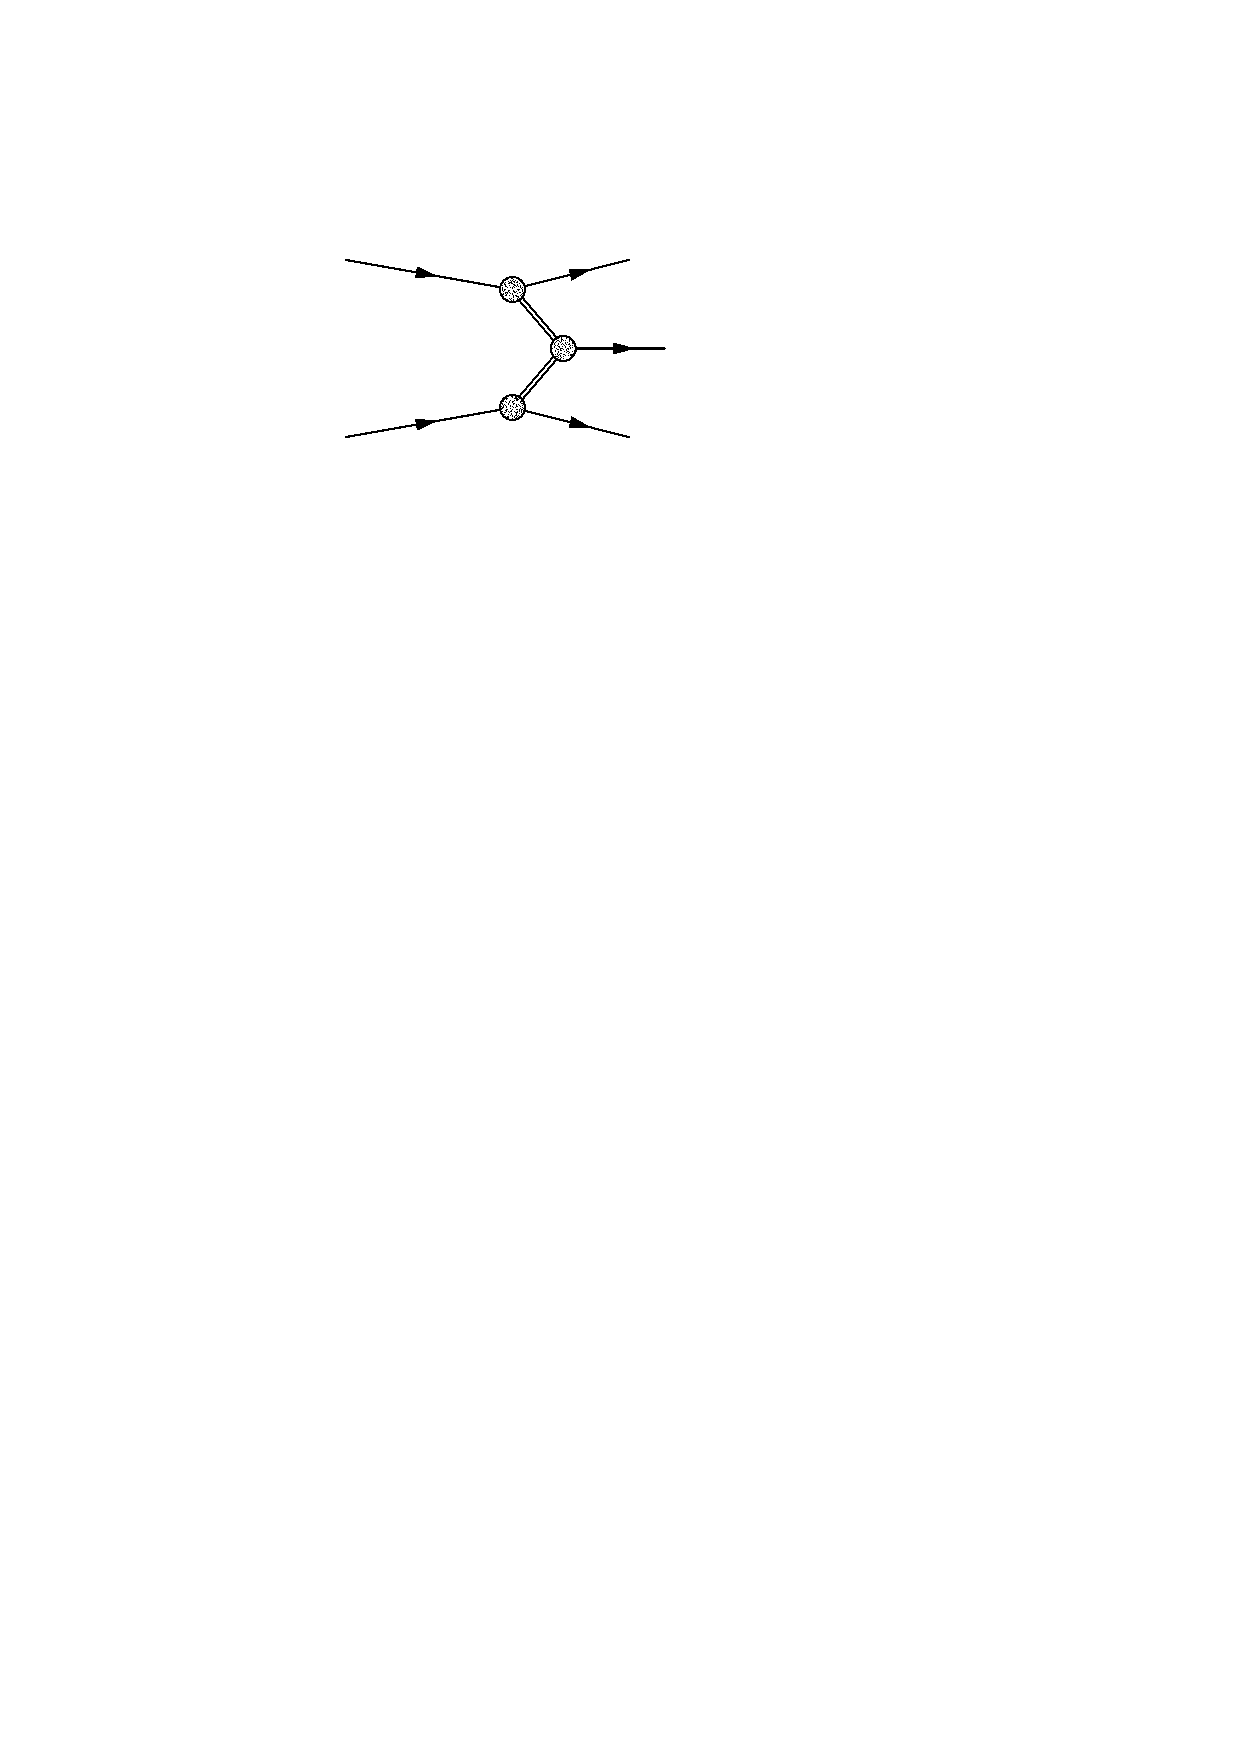
\includegraphics[height=3cm,keepaspectratio]{pics/CEP1.pdf}};
        % \node[align = center, above = of cep, yshift=-15mm] {\small CEP};
        \node[below=of cep, xshift=18mm,yshift=28mm] (X) {\small \emph{X}};
        \node[align = center, right = of X, xshift=0mm,yshift=5mm] (part1) {\small $\pi^{-}$};
        \node[align = center, right = of X, xshift=0mm,yshift=-5mm] (part2) {\small $\pi^{+}$};
        \draw[->,thick] (X) -- (part1);
        \draw[->,thick] (X) -- (part2);

        \node[inner sep=0pt] (cep2) at (0,-3) {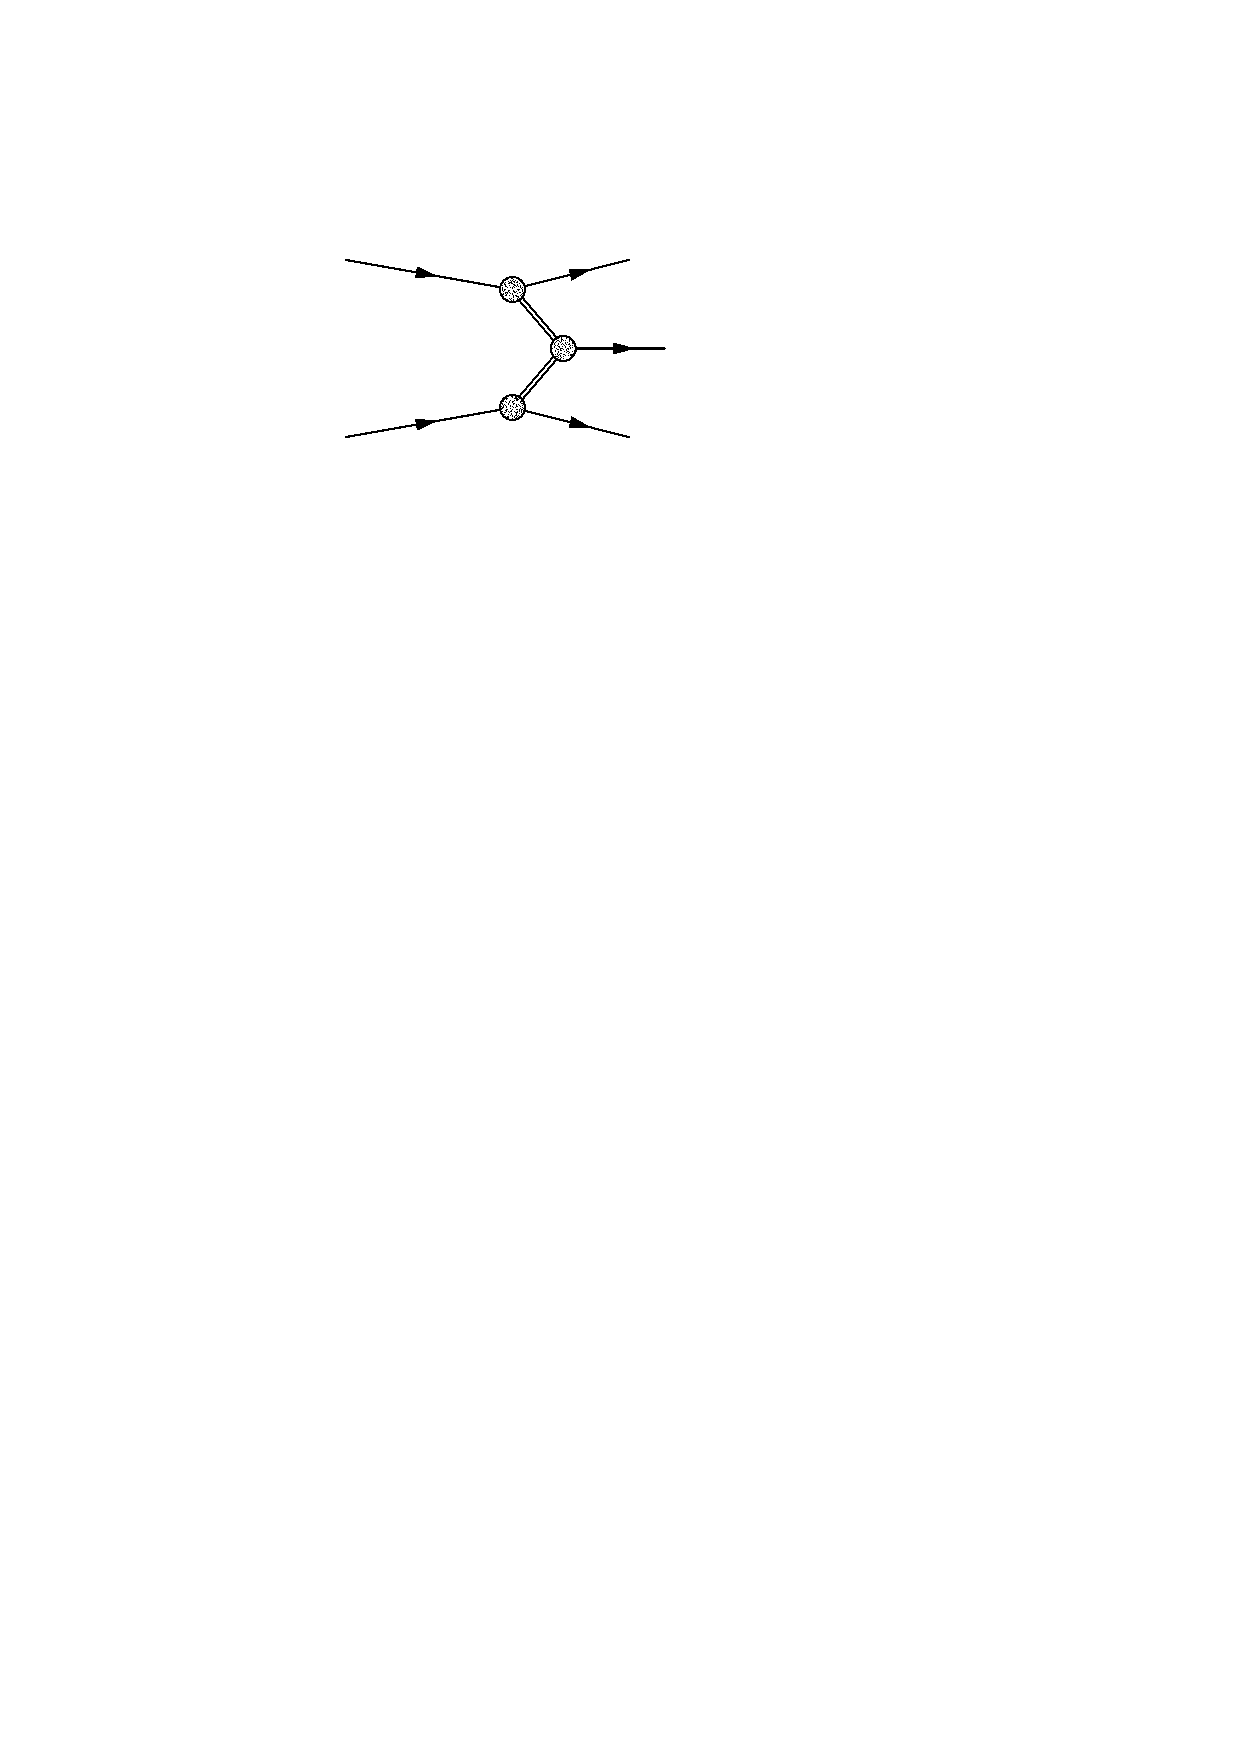
\includegraphics[height=3cm,keepaspectratio]{pics/CEP1.pdf}};
        \node[draw,rectangle,minimum height=28mm,minimum width=65mm,color=red,ultra thick,dashed] (rect) at (1,-3) {};
        \node[align = center, right = of rect, xshift=-10mm,yshift=0mm,text width=4cm] (txtFD) {\small $\pi^{0}$ not detectable ~$\to$~missing mass};
        \node[align = center, above = of txtFD, xshift=0mm,yshift=10mm,text width=4cm] (txtFR) {\small Total mass of $X$ recontructable};

        \node[below=of cep2, xshift=18mm,yshift=28mm] (X2) {\small \emph{X}};
        \node[align = center, right = of X2, xshift=0mm,yshift=8mm] (partFD1) {\small $\pi^{-}$};
        \node[align = center, right = of X2, xshift=0mm,yshift=0mm] (partFD2) {\small $\pi^{+}$};
        \node[align = center, right = of X2, xshift=0mm,yshift=-8mm] (part3) {\small $\pi^{0}$};
        \draw[->,thick] (X2) -- (partFD1);
        \draw[->,thick] (X2) -- (partFD2);
        \draw[->,thick,dashed] (X2) -- (part3);
    \end{tikzpicture}
\end{frame}

%------------------------------------------------ 
{\setbeamercolor{background canvas}{bg=red!20}
\begin{frame}
    \frametitle{Motivation}
    \begin{itemize}
        \item Reduce dominant background contribution: \textbf{feed down}\\\hspace*{5mm}$\to$~Try multivariate approach instead of classical cut methods\\\vspace*{5mm}
        \item Next up
        \begin{itemize}
            \item Comparison: Multi-variate \emph{vs.} single-variate analysis
        \end{itemize}
     \end{itemize}
\end{frame}
}

%------------------------------------------------ 

\section{ML: an overview} %

\begin{frame}
    \frametitle{ML: an overview}
    In general ML represents a contrast to a \emph{rule based systems}
    \begin{block}{Rule-based system}
        System that uses rules to make deductions or choices
        \begin{itemize}
            \item<1-> Domain-specific expert system
            \item<2-> Knowledge base: facts \& rules (if $\to$ then statement)
            \item<3-> Rules manually specified (by expert) $\to$ expensive, incomplete
        \end{itemize}
    \end{block}
\end{frame}

%------------------------------------------------ 

\begin{frame}
    \frametitle{ML: an overview}
    In general ML represents a contrast to a \emph{rule based systems}
    \begin{block}{Machine learning}
        \begin{itemize}
            \item<1-> Alorithms that learn from \emph{data} \& make predictions on \emph{data}
            \item<2-> Automatic methods $\to$ no human needed
            \item<3-> Human work required for defining problem \& assessing the data
        \end{itemize}
    \end{block}
\end{frame}

%------------------------------------------------ 

\begin{frame}
    \frametitle{Types of ML}
    \begin{columns}[T] % align columns
        \begin{column}{.48\textwidth}
            % \color{red}\rule{\linewidth}{4pt}

            \begin{itemize}
                \item <1->Supervised 
                \begin{itemize}
                    \item Classification
                    \item Regression
                \end{itemize}
                \item<2-> Unsupervised
            \end{itemize}
        \end{column}%
        \hfill%
        \begin{column}{.48\textwidth}
            \includegraphics<1>[height=4.5cm,keepaspectratio]{pics/supervised.png}%
            \includegraphics<2>[height=4.5cm,keepaspectratio]{pics/UNsupervised.png}%
            % \includegraphics<1>[height=3.5cm,keepaspectratio]{pics/supervised.png}\\%
            % \includegraphics<2>[height=3.5cm,keepaspectratio]{pics/UNsupervised.png}%
        \end{column}%
    \end{columns}
\end{frame}

%------------------------------------------------ 

\subsection{Rectangular cuts} %
\begin{frame}
    \frametitle{Rectangular cuts}
    \begin{columns}[T] % align columns        
        \begin{column}{.48\textwidth}
            % \color{red}\rule{\linewidth}{4pt}
            \vspace*{-10mm}
            Standard cut in one variable
            \begin{itemize}
                \item<1-> Cuts only in lower-dimensional subspaces
                \item<2-> Ignores possible dependencies between the input variables
                \item<3-> Signal might behave like BG in several observables\\ $\to$ misclassification
            \end{itemize}
        \end{column}%
        \hfill%
        \begin{column}{.48\textwidth}
            % \color{blue}\rule{\linewidth}{4pt}
            \vspace*{-10mm}
            % \hspace*{-10mm}
            \raggedright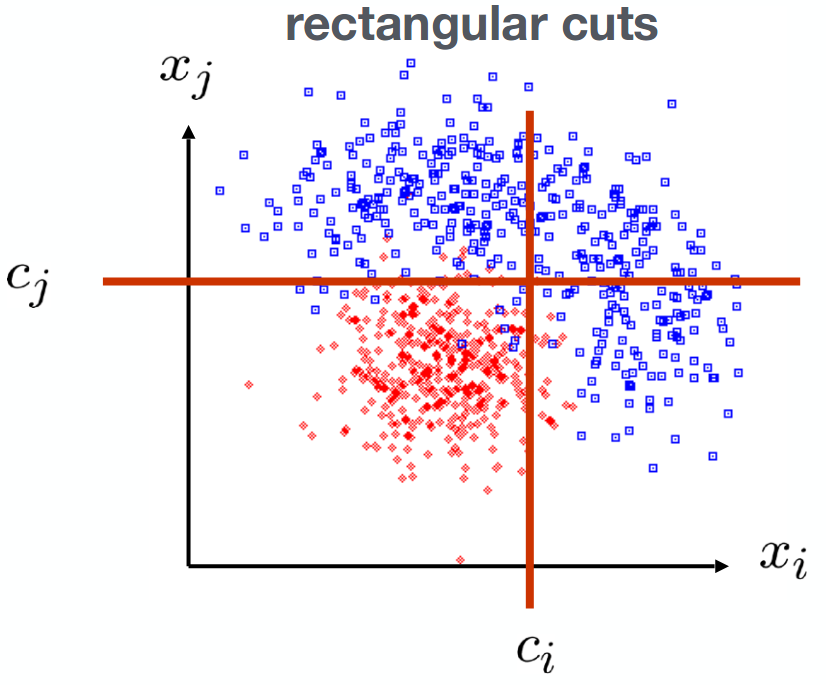
\includegraphics[height=4.3cm,keepaspectratio]{pics/mva_cuts_rectangular.png}%
            
        \end{column}%
    \end{columns}

\end{frame}

%------------------------------------------------ 

\begin{frame}
    \frametitle{Rectangular cuts with \emph{decision trees}}
    \vspace*{-7mm}
    \begin{itemize}
        % \item Simple \& rather old model (\emph{60s, 70s})
        \item Tree-like graph $\to$ flowchart
        \item Easy to understand
        \item Either be manually modelled by experts or learned from training data
    \end{itemize}
\end{frame}

%------------------------------------------------ 

% \begin{frame}
%     \frametitle{Rectangular cuts with \emph{decision trees}}
%     \begin{tikzpicture}
%         [
%             grow                    = right,
%             sibling distance        = 6em,
%             level distance          = 10em,
%             edge from parent/.style = {draw, -latex},
%             every node/.style       = {font=\footnotesize},
%             sloped
%         ]
% 	\node [root] {Student?}
%         child { node [dummy] {Exam?}
%                 child { node [env] {Beer}
%                         edge from parent node [above] {No} }
%                 child { node [env] {No Beer}
%                         edge from parent node [above] {Yes} }                
%                 edge from parent node [above] {Yes} }
%         child { node [dummy] {Weekday?}
%                 child { node [env] {No Beer}
%                         edge from parent node [above] {Yes} }
%                 child { node [env] {Beer}
%                         edge from parent node [above] {No} }                
%                 edge from parent node [above] {No} };
%     \pause
%     \node (rectroot) at (0,0) [rectangle, dashed, color=red, minimum height=2cm,minimum width=3cm,draw, thick] {};
%     \node (rootbottom) [below=1mm of rectroot, color=red]  {Root node};
%     \pause
%     \node (rectinner) at (3.8,0) [rectangle, dashed, color=red, minimum height=6cm,minimum width=2cm,draw, thick] {};
%     \node (innerbottom) [below=1mm of rectinner, color=red]  {Inner nodes};
%     \node (innertop) [above=1mm of rectinner, color=red]  {Decisions};
%     \pause
%     \node (rectleaf) at (7.7,0) [rectangle, dashed, color=red, minimum height=6cm,minimum width=2cm,draw, thick] {};
%     \node (leafbottom) [below=1mm of rectleaf, color=red]  {Leaf nodes};
%     \node (leaftop) [above=1mm of rectleaf, color=red]  {Class prediction};

%     \end{tikzpicture}
% \end{frame}

%------------------------------------------------ 

% \begin{frame}
%     \frametitle{Decision tree learning}
%     \vspace*{-7mm}
%     \begin{block}{Training}
%         \emph{Recursively} split feature space into sub-spaces at each step\\
%         $\to$ Measures to evaluate split
%         \begin{itemize}
%             \item Error rate
%             \item Information gain
%             \item Gini index
%         \end{itemize}
%     \end{block}
% \end{frame}

%------------------------------------------------ 

\begin{frame}
    \frametitle{Decision tree learning}
    \centering\begin{tikzpicture}
        \node[inner sep=0pt] (featspace) at (0,0)
            {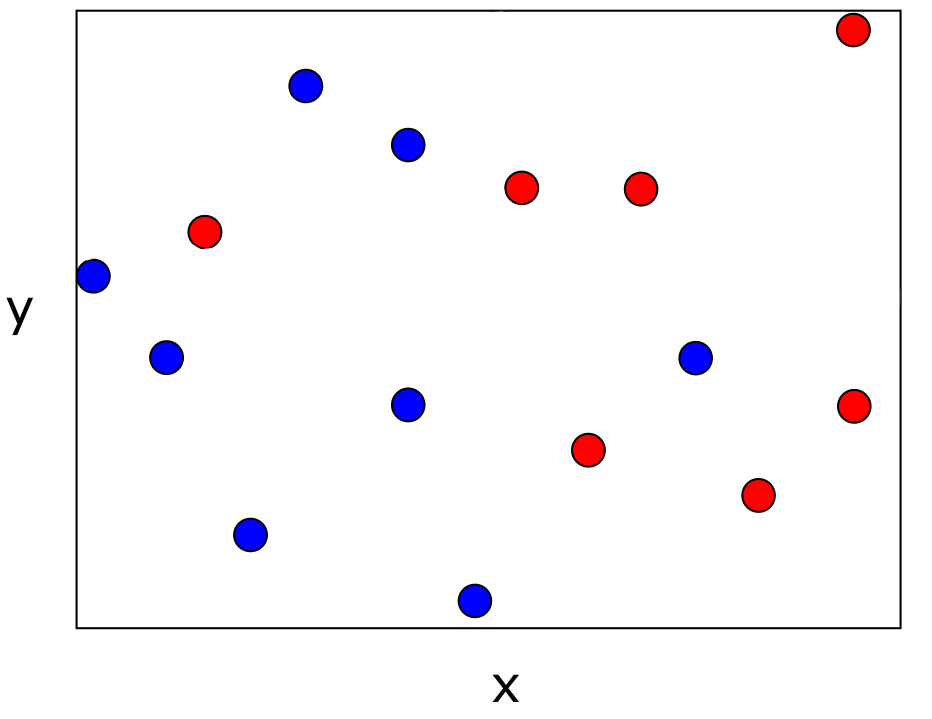
\includegraphics[height=3cm,keepaspectratio]{pics/DT-feature-space.png}};
        \node (featspaceTop) [above=1mm of featspace, color=black]  {Feature space};
        \node[inner sep=0pt] (nodes) at (3,-3.5)
            {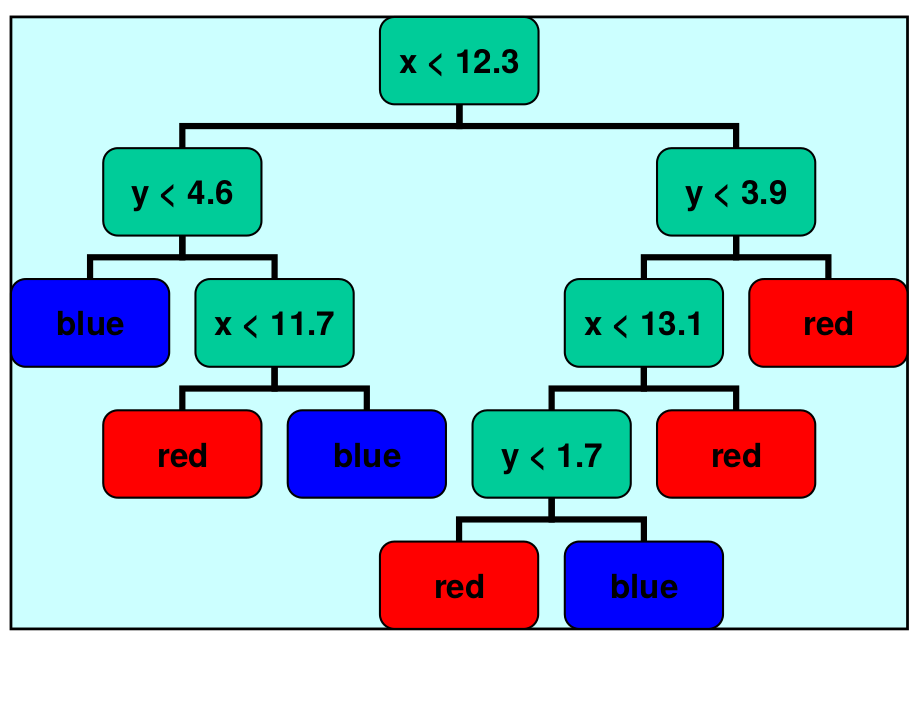
\includegraphics[height=3.3cm,keepaspectratio]{pics/DT-fullygrown_nodes.png}};%
        \node (nodesTxt) [above=1mm of nodes, color=black]  {Decision tree};
        \node[inner sep=0pt] (DTapply) at (-3,-3.5)
            {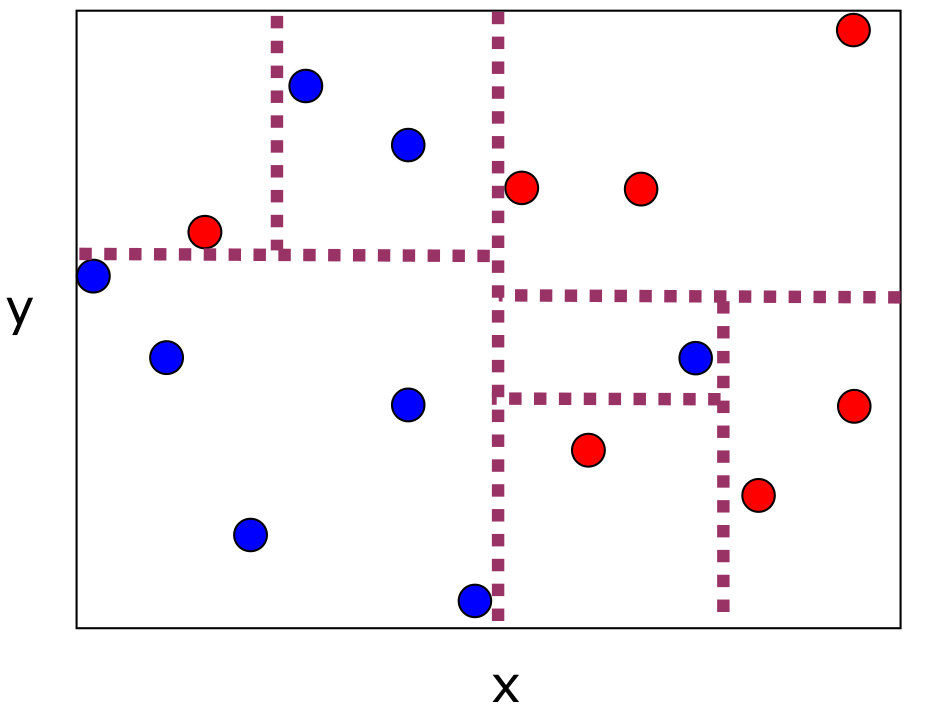
\includegraphics[height=3.3cm,keepaspectratio]{pics/DT-fullygrown_feature_space.png}};
        \node (DTTxt) [above=1mm of DTapply, color=black]  {Classification};

        \draw[->,thick] (featspace.east) to [out=0,in=90] (nodesTxt.north) node[midway,above] {};
        \draw[->,thick] (featspace.west) to [out=180,in=90] (DTTxt.north) node[midway,above] {};
    \end{tikzpicture}
\end{frame}

%------------------------------------------------ 

\begin{frame}
    \frametitle{Decision tree learning}
    1) We compute a measure for \emph{each possible split} in each feature\\\hspace*{5mm}$\to$ here \textbf{absolute error rate} (AER)
    \\
    \vspace*{3mm}
    \centering\begin{tikzpicture}
        \node[inner sep=0pt, visible on=<1>] (feat1) at (0,0)
            {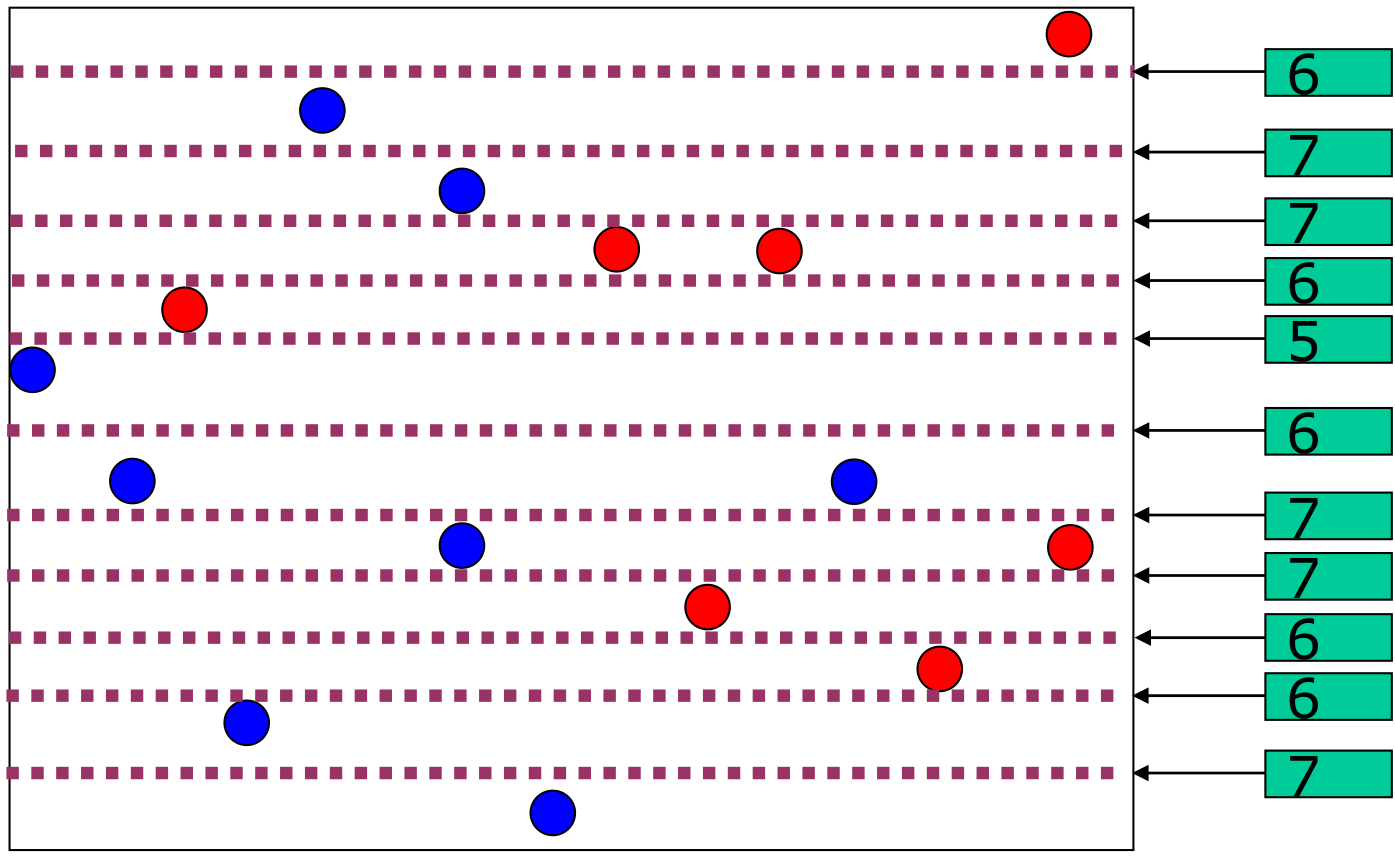
\includegraphics[height=4.5cm,keepaspectratio]{pics/DT-ER-y.png}};
        \node (feat1Txt) [above=1mm of feat1, color=black]  {\emph{y} split AER};
        % \node[inner sep=0pt, visible on=<2>] (feat2) at (0,0)
        %     {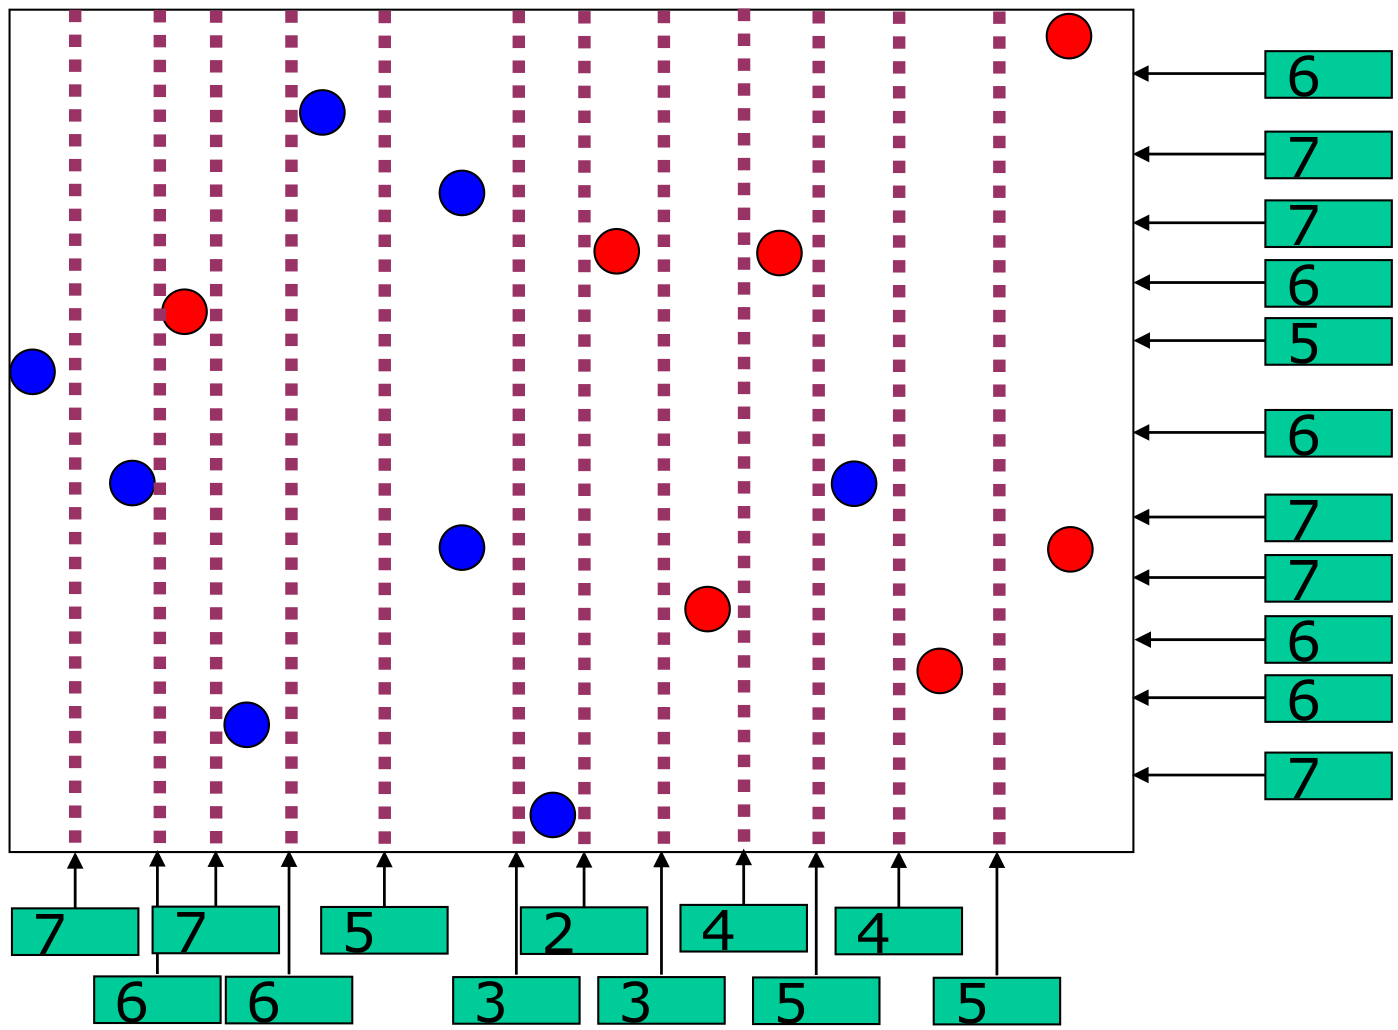
\includegraphics[height=4.5cm,keepaspectratio]{pics/DT-ER-x.png}};
        % \node (feat2Txt) [above=1mm of feat1, color=black,visible on=<2>]  {\emph{x}-\emph{y} split AER};
    \end{tikzpicture}
 
\end{frame}

%------------------------------------------------ 

\begin{frame}
    \frametitle{Decision tree learning}
    1) We compute a measure for \emph{each possible split} in each feature\\\hspace*{5mm}$\to$ here \textbf{absolute error rate} (AER)
    \\
    \vspace*{3mm}
    \centering\begin{tikzpicture}
        \node[inner sep=0pt] (feat2) at (0,0)
            {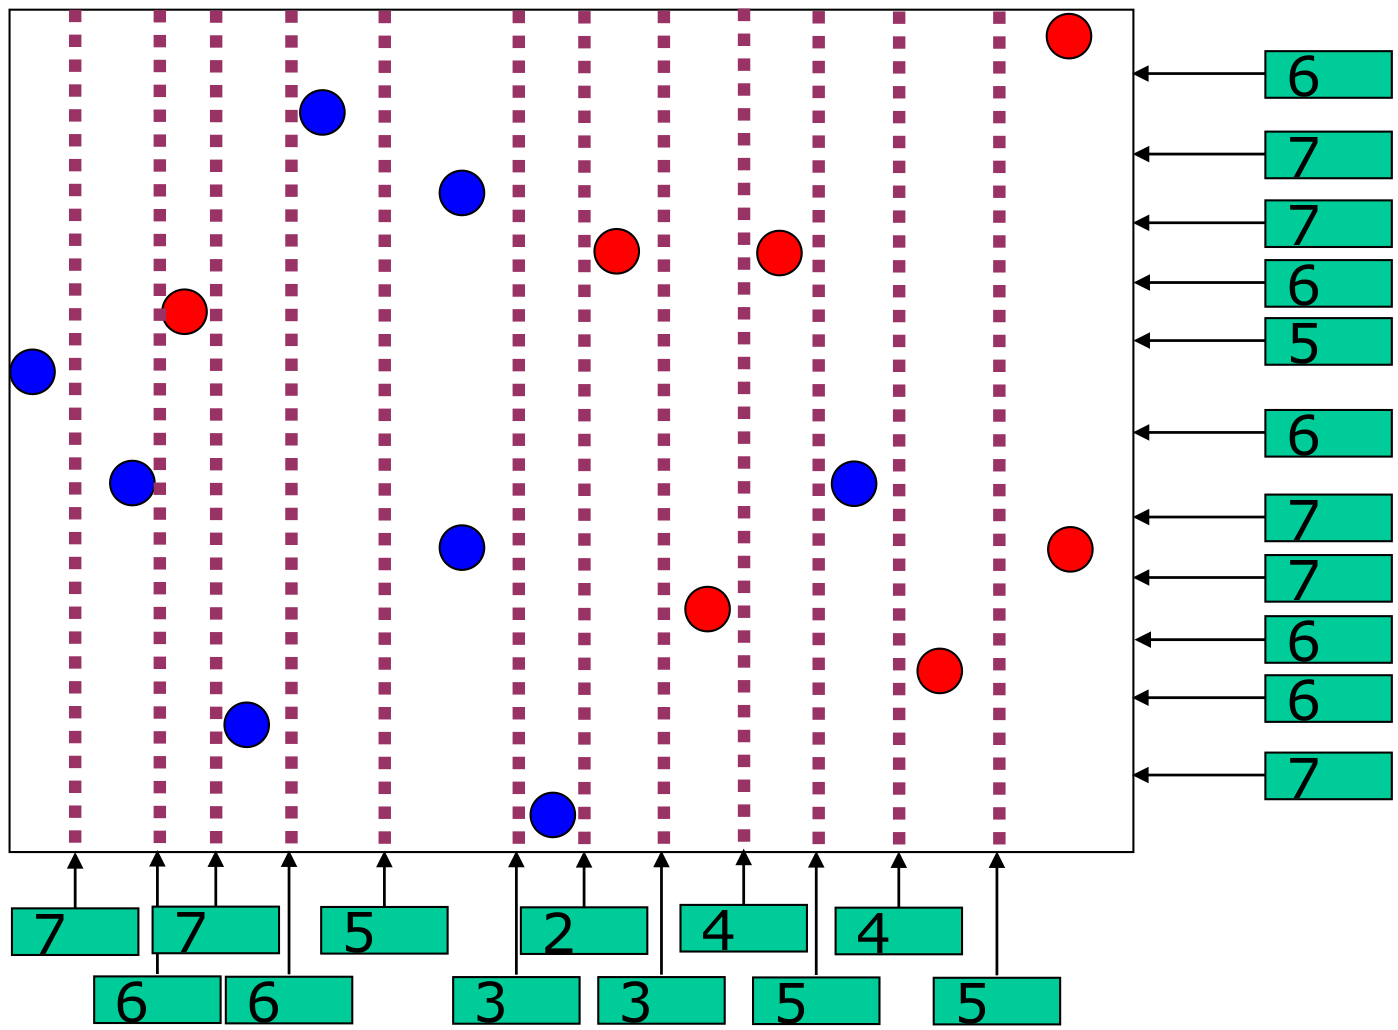
\includegraphics[height=4.5cm,keepaspectratio]{pics/DT-ER-x.png}};
        \node (feat2Txt) [above=1mm of feat1, color=black]  {\emph{x}-\emph{y} split AER};
        \pause
        \node (el) at (-0.53,-1.8) [ellipse, color=red, minimum height=5mm,minimum width=10mm,draw, ultra thick] {};
        \node (txt) at (3.5,-1.8) [color=red, ultra thick] {Minimum AER};
        \draw[->, color=red, ultra thick] (txt) to [out=160, in=20] (el);

    \end{tikzpicture}
 
\end{frame}

%------------------------------------------------ 

\begin{frame}
    \frametitle{Decision tree learning}
    1) We compute a measure for \emph{each possible split} in each feature\\\hspace*{5mm}$\to$ here \textbf{absolute error rate} (AER)\\
    2) Recursively repead step (1) for each subspace until AER $\to 0$
    \\
    \vspace*{3mm}
    \centering\includegraphics<1>[height=4.3cm,keepaspectratio]{pics/DT_1_split.png}%
    \centering\includegraphics<2>[height=4.6cm,keepaspectratio]{pics/DT_2_split.png}%
    \centering\includegraphics<3>[height=4.6cm,keepaspectratio]{pics/DT_3_split.png}%
    \centering\includegraphics<4>[height=4.6cm,keepaspectratio]{pics/DT_4_split.png}%
    \centering\includegraphics<5>[height=4.6cm,keepaspectratio]{pics/DT_5_split.png}%
    \centering\includegraphics<6>[height=4.3cm,keepaspectratio]{pics/DT_final.png}%
     
\end{frame}

%------------------------------------------------ 

\begin{frame}
    \frametitle{Decision tree classification}
    3) Classification
    \\
    \vspace*{3mm}
    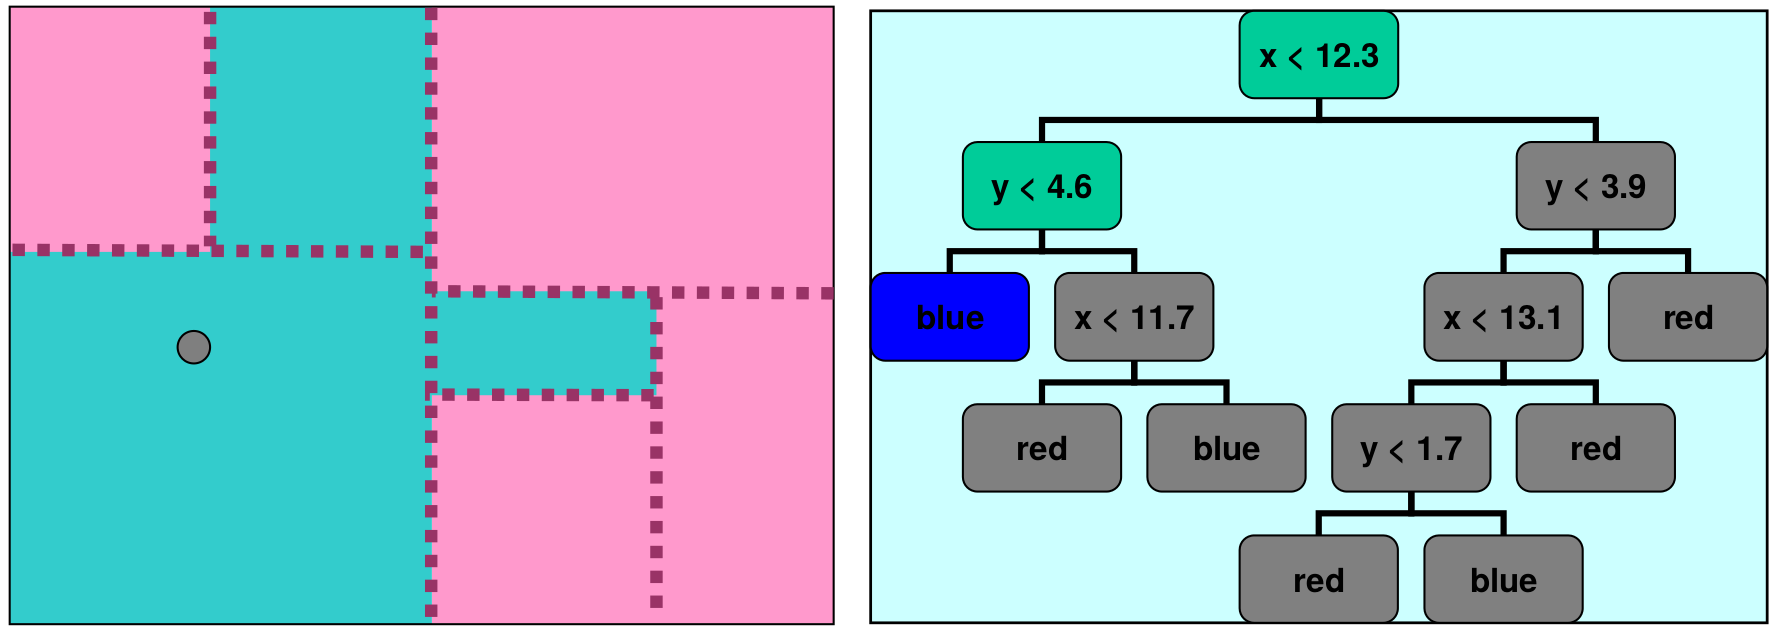
\includegraphics[height=4.3cm,keepaspectratio]{pics/DT_classification.png}%
 
\end{frame}

%------------------------------------------------ 

\begin{frame}
    \frametitle{Decision tree improvements I}
    \begin{itemize}
        \item Use more sophisticated split measures 
            \begin{itemize}
                \item \emph{Information gain} $\leftrightarrow$ (im-)purity of splitted sub-sets
            \end{itemize}
        \item Pruning 
        \item Ensemble trees (Random forest \& boosted DT)
    \end{itemize}
    \vspace*{3mm}
    \centering\begin{tikzpicture}
        \node[inner sep=0pt] (IG) at (3,0)
            {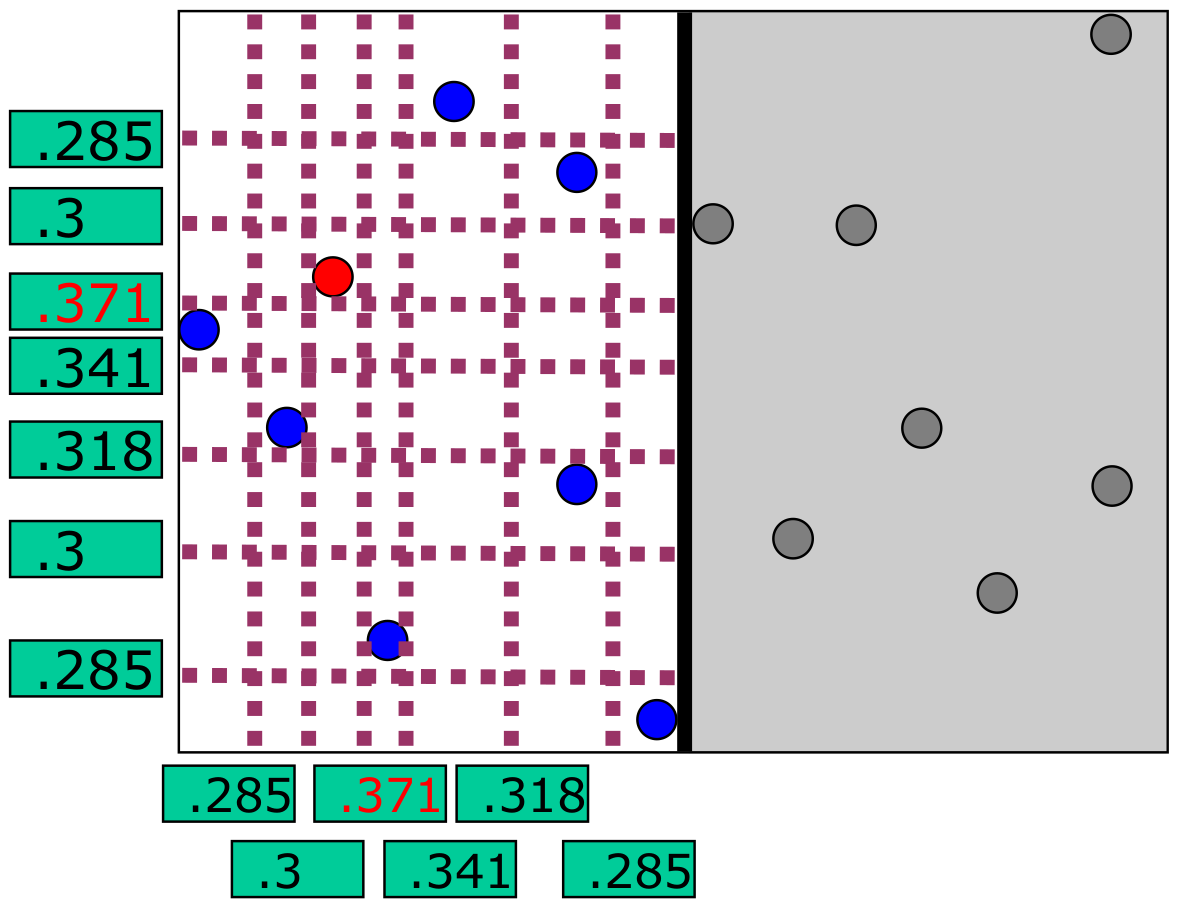
\includegraphics[height=3.5cm,keepaspectratio]{pics/DT_info-gain.png}};
        \node (IGtxt) [below=1mm of IG, color=black]  {Information gain};
        \node[inner sep=0pt] (AER) at (-3,0)
            {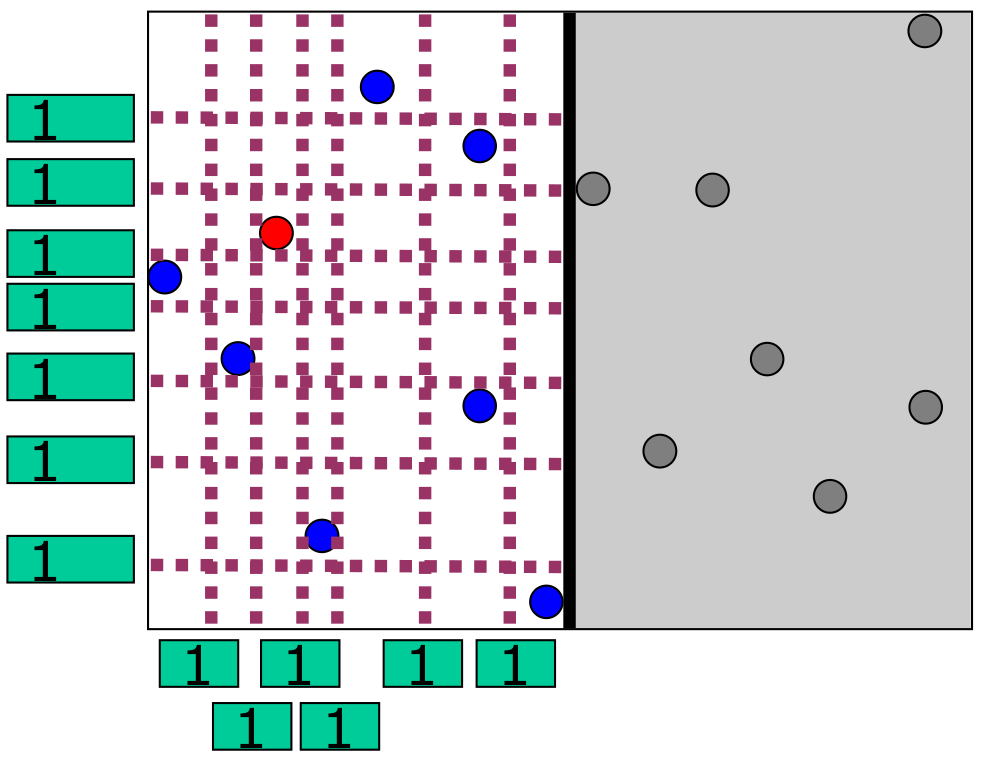
\includegraphics[height=3.5cm,keepaspectratio]{pics/DT_AER.png}};
        \node (AERtxt) [below=1mm of AER, color=black]  {Absolute error rate};
        \draw[->, color=red, ultra thick] (AER) to [out=0, in=180] (IG);
    \end{tikzpicture}
 
\end{frame}

%------------------------------------------------ 

% \begin{frame}
%     \frametitle{Decision tree improvements II}
%     \begin{columns}[T] % align columns        
%         \begin{column}{.48\textwidth}
%             \begin{block}{Random forest}
%                 \begin{itemize}
%                     \item<1-> Ensemble of DTs
%                     \item<2-> For each tree use:
%                     \begin{itemize}
%                         \item<3-> Random sub-sample (=\emph{bootstrapping})
%                         \item<4-> Random number of the original features\\
%                                   $\to$ large number of rather shallow trees
%                     \end{itemize}
%                     \item<5-> Classify data by majority voting of individual trees
%                 \end{itemize}
%             \end{block}
%         \end{column}%
%         \hfill%
%         \begin{column}{.48\textwidth}
%             \begin{block}{Boosted DT}
%                 \begin{itemize}
%                     \item<6-> Sequential ensemble of evolving DTs
%                     \item<7-> Assign weights to training samples $\to$ initially equal weights
%                     \item<8-> Adjust weights \& give more importance to misclassified samples
%                     \item<9-> Subsequent predictors thus should focus on those 
%                 \end{itemize}
%             \end{block}            
%         \end{column}%
%     \end{columns}

% \end{frame}

%------------------------------------------------ 

\subsection{Linear cuts}

\begin{frame}
    \frametitle{Linear cuts}
    \begin{columns}[T] % align columns        
        \begin{column}{.48\textwidth}
            % \color{red}\rule{\linewidth}{4pt}
            More degrees of freedom than rectangular cut
            \begin{itemize}
                \item<1-> Simple white box methods 
                \item<2-> Very fast classification
                \item<3-> Can become very powerful by using \emph{kernel trick}
            \end{itemize}
        \end{column}%
        \hfill%
        \begin{column}{.48\textwidth}
            % \color{blue}\rule{\linewidth}{4pt}
            % \hspace*{-10mm}
            \raggedright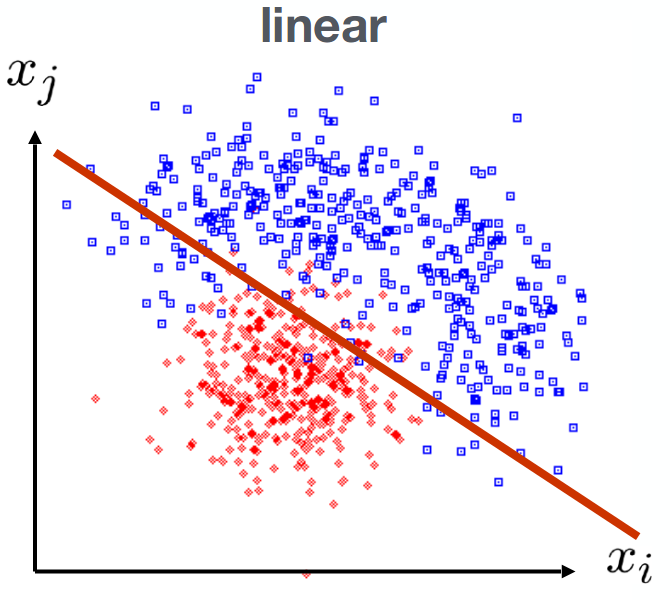
\includegraphics[height=4.3cm,keepaspectratio]{pics/mva_cut_linear.png}%
            
        \end{column}%
    \end{columns}

\end{frame} 

%------------------------------------------------ 

\begin{frame}
    \frametitle{Linear models}
    Takes a \emph{linear function} of its inputs $\boldsymbol{x} = (x_{1},\dots x_{n})$ to base its decision on.\\
    % $$ y = f ( \boldsymbol{w} \cdot \boldsymbol{x}) = f \left\( \sum_{j}w_{j}x_{j} \right\) $$
    $$ y: \mathbb{R}^{n} \to \mathbb{R}~|~\boldsymbol{x} \mapsto y = f (\boldsymbol{w} \cdot \boldsymbol{x}) = f (\sum_{j}w_{j}x_{j}) $$
    
    $\boldsymbol{w}\dots$ weight vector\\ 
    \vspace*{4mm}

    \pause
    Simplest case
    \[ 
         y = f(x)=\Theta(x)=
         \begin{cases} 
             0 & x < 0 \hspace*{5mm}\text{signal}\\
             1  & x \geq 0 \hspace*{5mm}\text{background}
        \end{cases} 
    \] 
    \pause
    \hspace*{5mm}$\to$ Function can be approximated by \textbf{single layer perceptron}
     % Maps all values above certain threshold to \emph{signal} and all others to \emph{background}
    
\end{frame} 

%------------------------------------------------ 
\begin{frame}
    \frametitle{Single layer perceptron (SLP)}

    \centering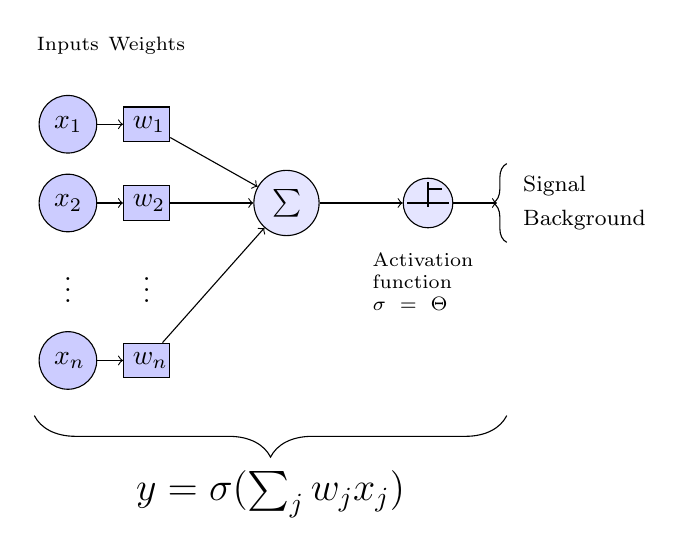
\begin{tikzpicture}
        \node[functions] (center) {};
        \node[below of=center,font=\scriptsize,text width=4em] {Activation function $\sigma~=~\Theta$};
        \draw[thick] (0.5em,0.5em) -- (0,0.5em) -- (0,0) -- (-0.5em,0);
        \draw (0em,0.75em) -- (0em,-0.15em);
        \draw (0.75em,0em) -- (-0.75em,0em);
        \node[right of=center] (right) {};
            \path[draw,->] (center) -- (right);
        \node[functions,left=3em of center] (left) {$\sum$};
            \path[draw,->] (left) -- (center);
        \node[weights,left=3em of left] (2) {$w_{2}$} -- (2) node[input,left of=2] (l2) {$x_{2}$};
            \path[draw,->] (l2) -- (2);
            \path[draw,->] (2) -- (left);
        \node[below of=2] (dots) {$\vdots$} -- (dots) node[left of=dots] (ldots) {$\vdots$};
        \node[weights,below of=dots] (n) {$w_{n}$} -- (n) node[input,left of=n] (ln) {$x_{n}$};
            \path[draw,->] (ln) -- (n);
            \path[draw,->] (n) -- (left);
        \node[weights,above of=2] (1) {$w_{1}$} -- (1) node[input,left of=1] (l1) {$x_{1}$};
            \path[draw,->] (l1) -- (1);
            \path[draw,->] (1) -- (left);
        % \node[weights,above of=1] (0) {$w_{0}$} -- (0) node[input,left of=0] (l0) {$1$};
        %     \path[draw,->] (l0) -- (0);
        %     \path[draw,->] (0) -- (left);
        \node[above of=l1,font=\scriptsize] {Inputs};
        \node[above of=1,font=\scriptsize] {Weights};
        \draw [decorate,decoration={brace,mirror,amplitude=15pt},xshift=0pt,yshift=0pt]
            (-5,-2.7) -- (1,-2.7) node [black,midway,yshift=-1.0cm] 
            {\Large $y = \sigma(\sum_{j}w_{j}x_{j})$};
            % {\Large $y: \boldsymbol{x} \mapsto y = \Theta(\sum_{j}w_{j}x_{j})$};
            % {$y: \mathbb{R}^{n} \to \mathbb{R}$};
        \draw [decorate,decoration={brace,amplitude=5pt},xshift=0pt,yshift=0pt]
            (1,-0.5) -- (1,0.5) node [text width=4.5em,black,midway,xshift=1cm] 
            {\footnotesize Signal Background};
    \end{tikzpicture}
    
\end{frame} 

%------------------------------------------------ 

\begin{frame}
    \frametitle{SLP training}
    \begin{columns}[T] % align columns        
        \begin{column}{.48\textwidth}
            % \color{red}\rule{\linewidth}{4pt}
            \begin{block}{Algorithm} 
                \begin{enumerate}
                    \item Initialize weights $\boldsymbol{w}$
                    \item Repeat until $y_{predict}=y_{target}$:
                    \begin{enumerate}
                        \item Present training sample $\boldsymbol{x}$
                        \item Predict sample label $y=\Theta(\boldsymbol{x}\boldsymbol{w}_{init})$ and compute error $\Delta=y_{target}-y$
                        \item If $\Delta \neq 0~\to$ update weights\\$\boldsymbol{w}\textprime=\boldsymbol{w} + \alpha \Delta \boldsymbol{x}$
                    \end{enumerate}
                \end{enumerate}
            \end{block}
        \end{column}%
        \hfill%
        \begin{column}{.48\textwidth}
            % \color{blue}\rule{\linewidth}{4pt}
            % \hspace*{-10mm}
            \raggedright\includegraphics<1>[height=4.3cm,keepaspectratio]{pics/PCT_init_weights.png}%
            \raggedright\includegraphics<2>[height=4.3cm,keepaspectratio]{pics/PCT_0.png}%
            \raggedright\includegraphics<3>[height=4.3cm,keepaspectratio]{pics/PCT_1.png}%
            \raggedright\includegraphics<4>[height=4.3cm,keepaspectratio]{pics/PCT_2.png}%
            \raggedright\includegraphics<5>[height=4.3cm,keepaspectratio]{pics/PCT_3.png}%
            \raggedright\includegraphics<6>[height=4.3cm,keepaspectratio]{pics/PCT_final_0.png}%
            \raggedright\includegraphics<7>[height=4.3cm,keepaspectratio]{pics/PCT_regions.png}%

            \begin{textblock}{3.5}(10,13)
                $y = w_{1}x_{1} + w_{2}x_{2}$
            \end{textblock}
            \only<3-> {
                \begin{textblock}{5}(2,13)
                    $\alpha \dots$~learning rate
                \end{textblock}
            }
                 
        \end{column}%
    \end{columns}

\end{frame} 

%------------------------------------------------ 
\begin{frame}
    \frametitle{SLP bias term}
    \begin{columns}[T] % align columns        
        \begin{column}{.48\textwidth}
            \pause
            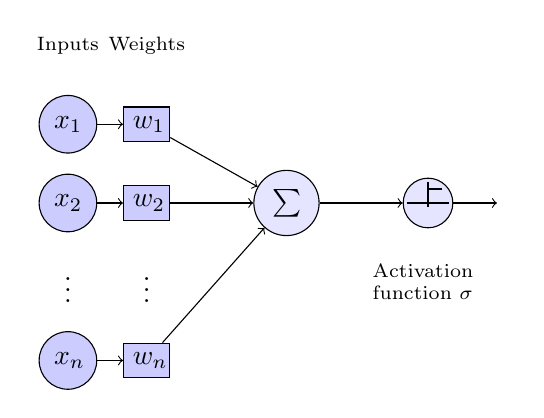
\begin{tikzpicture}
                \node[functions] (center) {};
                \node[below of=center,font=\scriptsize,text width=4em] {Activation function $\sigma$};
                \draw[thick] (0.5em,0.5em) -- (0,0.5em) -- (0,0) -- (-0.5em,0);
                \draw (0em,0.75em) -- (0em,-0.15em);
                \draw (0.75em,0em) -- (-0.75em,0em);
                \node[right of=center] (right) {};
                    \path[draw,->] (center) -- (right);
                \node[functions,left=3em of center] (left) {$\sum$};
                    \path[draw,->] (left) -- (center);
                \node[weights,left=3em of left] (2) {$w_{2}$} -- (2) node[input,left of=2] (l2) {$x_{2}$};
                    \path[draw,->] (l2) -- (2);
                    \path[draw,->] (2) -- (left);
                \node[below of=2] (dots) {$\vdots$} -- (dots) node[left of=dots] (ldots) {$\vdots$};
                \node[weights,below of=dots] (n) {$w_{n}$} -- (n) node[input,left of=n] (ln) {$x_{n}$};
                    \path[draw,->] (ln) -- (n);
                    \path[draw,->] (n) -- (left);
                \node[weights,above of=2] (1) {$w_{1}$} -- (1) node[input,left of=1] (l1) {$x_{1}$};
                    \path[draw,->] (l1) -- (1);
                    \path[draw,->] (1) -- (left);
                % \node[weights,above of=1] (0) {$w_{0}$} -- (0) node[input,left of=0] (l0) {$1$};
                %     \path[draw,->] (l0) -- (0);
                %     \path[draw,->] (0) -- (left);
                \node[above of=l1,font=\scriptsize] {Inputs};
                \node[above of=1,font=\scriptsize] {Weights};
            \end{tikzpicture}
        \end{column}%
        \hfill%
        \begin{column}{.48\textwidth}
            \hspace*{2mm}
            \raggedright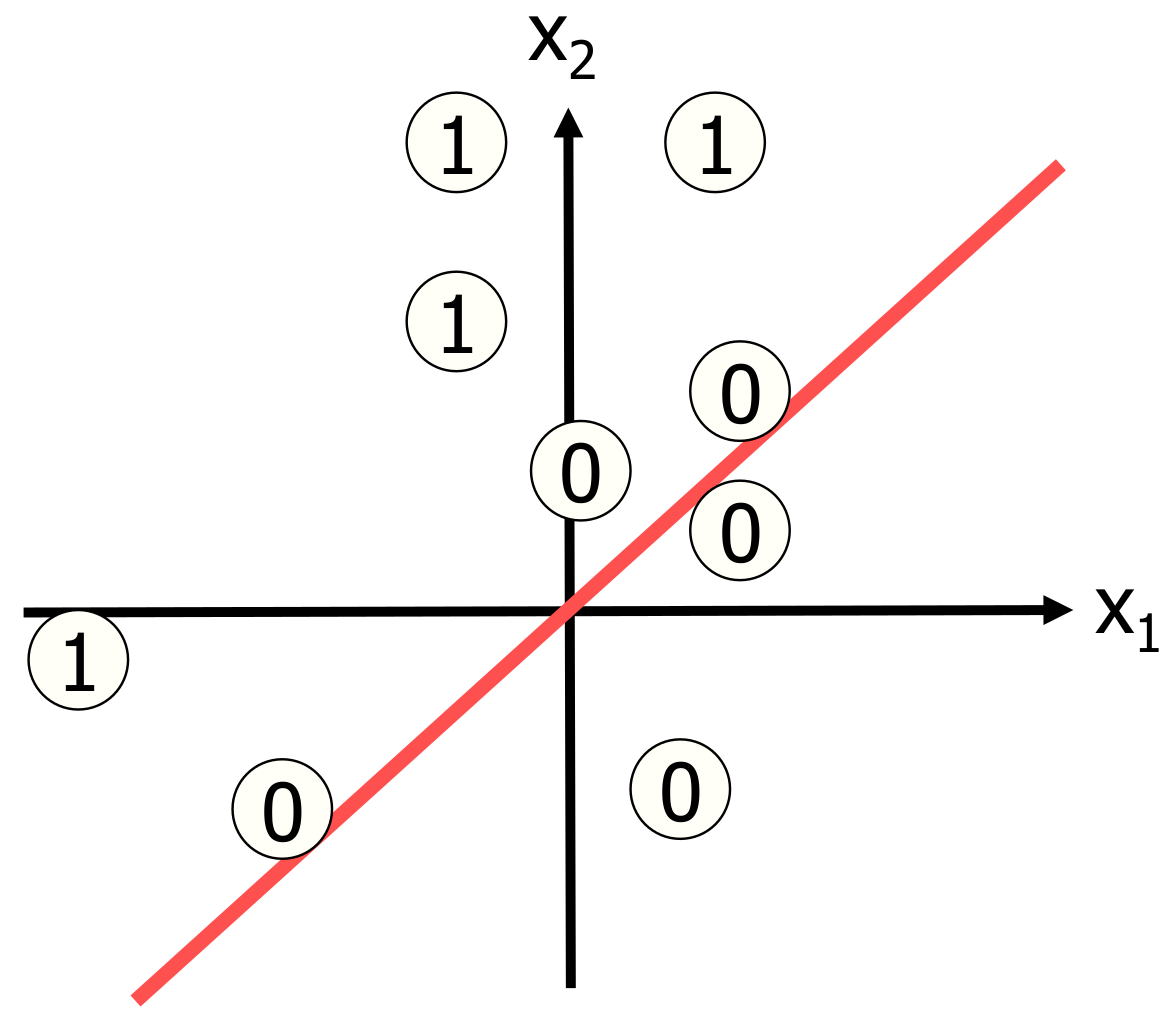
\includegraphics[height=4.3cm,keepaspectratio]{pics/PCT_no_bias.png}%            
        \end{column}% 
    \end{columns}
\end{frame}

%------------------------------------------------ 

\begin{frame}
    \frametitle{SLP bias term}
    \begin{columns}[T] % align columns        
        \begin{column}{.48\textwidth}
            \vspace*{-10mm}
            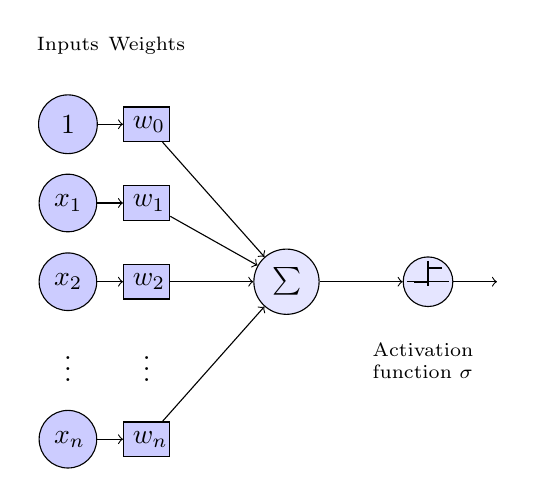
\begin{tikzpicture}
                \node[functions] (center) {};
                \node[below of=center,font=\scriptsize,text width=4em] {Activation function $\sigma$};
                \draw[thick] (0.5em,0.5em) -- (0,0.5em) -- (0,0) -- (-0.5em,0);
                \draw (0em,0.75em) -- (0em,-0.15em);
                \draw (0.75em,0em) -- (-0.75em,0em);
                \node[right of=center] (right) {};
                    \path[draw,->] (center) -- (right);
                \node[functions,left=3em of center] (left) {$\sum$};
                    \path[draw,->] (left) -- (center);
                \node[weights,left=3em of left] (2) {$w_{2}$} -- (2) node[input,left of=2] (l2) {$x_{2}$};
                    \path[draw,->] (l2) -- (2);
                    \path[draw,->] (2) -- (left);
                \node[below of=2] (dots) {$\vdots$} -- (dots) node[left of=dots] (ldots) {$\vdots$};
                \node[weights,below of=dots] (n) {$w_{n}$} -- (n) node[input,left of=n] (ln) {$x_{n}$};
                    \path[draw,->] (ln) -- (n);
                    \path[draw,->] (n) -- (left);
                \node[weights,above of=2] (1) {$w_{1}$} -- (1) node[input,left of=1] (l1) {$x_{1}$};
                    \path[draw,->] (l1) -- (1);
                    \path[draw,->] (1) -- (left);
                \node[weights,above of=1] (0) {$w_{0}$} -- (0) node[input,left of=0] (l0) {$1$};
                    \path[draw,->] (l0) -- (0);
                    \path[draw,->] (0) -- (left);
                \node[above of=l0,font=\scriptsize] {Inputs};
                \node[above of=0,font=\scriptsize] {Weights};
            \end{tikzpicture}
        \end{column}%
        \hfill%
        \begin{column}{.48\textwidth}
            \hspace*{2mm}
            \raggedright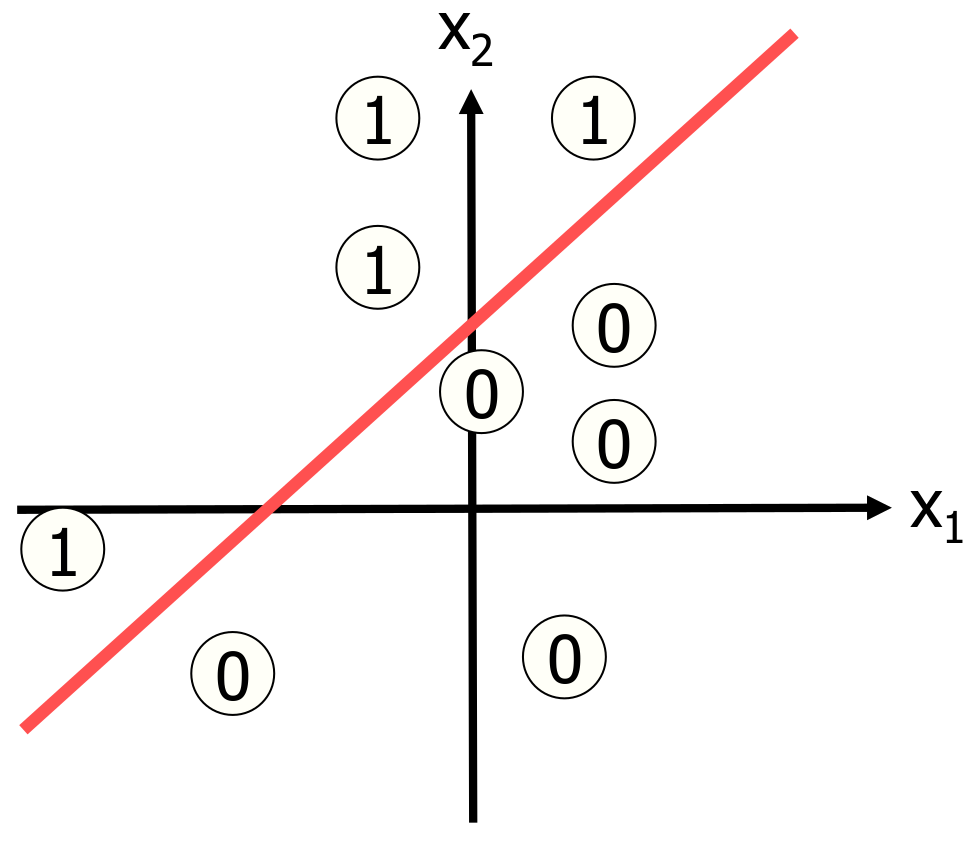
\includegraphics[height=4.3cm,keepaspectratio]{pics/PCT_with_bias.png}%            
        \end{column}% 
    \end{columns}
    \only<3-> {
        \begin{textblock}{10}(3,13)
            Bias weight $w_{0}$ learned just as the other weights\\\vspace*{1mm}
            \centering$ y = \sigma ( w_{0} + \sum_{j=1}^{n}w_{j}x_{j} ) $

        \end{textblock}
    }   

\end{frame}
% -----------------------------------------------

\begin{frame}
    \frametitle{SLP activation functions}
    \vspace*{-5mm}
    \begin{tikzpicture}
        \node[functions] (center) {};
        \node[below of=center,font=\scriptsize,text width=4em] {Activation function $\sigma$};
        \draw[thick] (0.5em,0.5em) -- (0,0.5em) -- (0,0) -- (-0.5em,0);
        \draw (0em,0.75em) -- (0em,-0.15em);
        \draw (0.75em,0em) -- (-0.75em,0em);
        \node[right of=center] (right) {};
            \path[draw,->] (center) -- (right);
        \node[functions,left=3em of center] (left) {$\sum$};
            \path[draw,->] (left) -- (center);
        \node[weights,left=3em of left] (2) {$w_{2}$} -- (2) node[input,left of=2] (l2) {$x_{2}$};
            \path[draw,->] (l2) -- (2);
            \path[draw,->] (2) -- (left);
        \node[below of=2] (dots) {$\vdots$} -- (dots) node[left of=dots] (ldots) {$\vdots$};
        \node[weights,below of=dots] (n) {$w_{n}$} -- (n) node[input,left of=n] (ln) {$x_{n}$};
            \path[draw,->] (ln) -- (n);
            \path[draw,->] (n) -- (left);
        \node[weights,above of=2] (1) {$w_{1}$} -- (1) node[input,left of=1] (l1) {$x_{1}$};
            \path[draw,->] (l1) -- (1);
            \path[draw,->] (1) -- (left);
        \node[weights,above of=1] (0) {$w_{0}$} -- (0) node[input,left of=0] (l0) {$1$};
            \path[draw,->] (l0) -- (0);
            \path[draw,->] (0) -- (left);
        \node[above of=l0,font=\scriptsize] {Inputs};
        \node[above of=0,font=\scriptsize] {Weights};

        \node (el) at (0,0) [ellipse, color=red, minimum height=10mm,minimum width=10mm,draw, ultra thick, dashed] {};
        \node[inner sep=0pt] (actfunc) at (4,0)
            {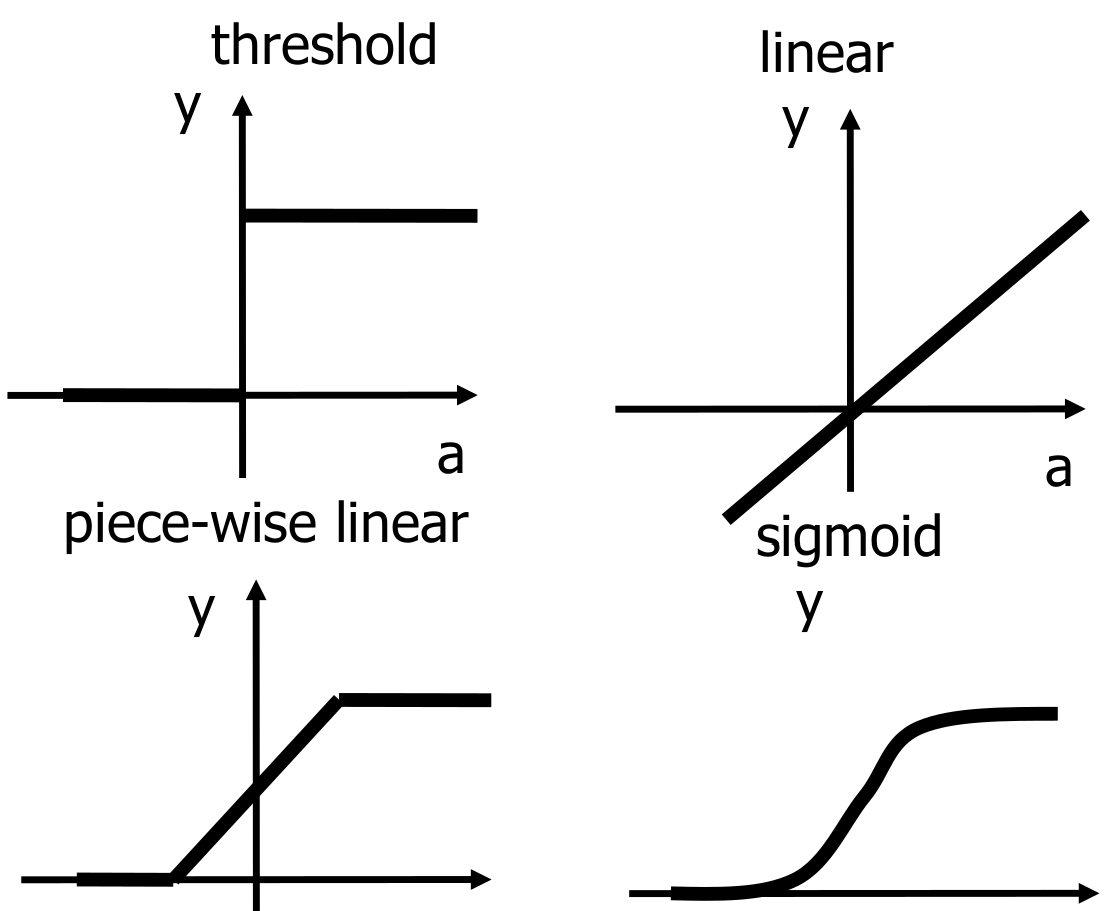
\includegraphics[height=3.3cm,keepaspectratio]{pics/activation_functions.png}};
        \draw[->, color=red, ultra thick] (actfunc) to [out=160, in=20] (el);
    \end{tikzpicture}

    \only<2-> {
        \begin{textblock}{10}(4,13)
            Often used: \emph{sigmoid} $\to$ output $\in (0,1)$
        \end{textblock}
    }   
\end{frame}

% -----------------------------------------------

\begin{frame}
    \frametitle{Non-linear activation functions: output}
    Distance to decision boundary comes into play
    \centering\begin{tikzpicture}
        \node<1>[inner sep=0pt] (theta) at (0,0)
            {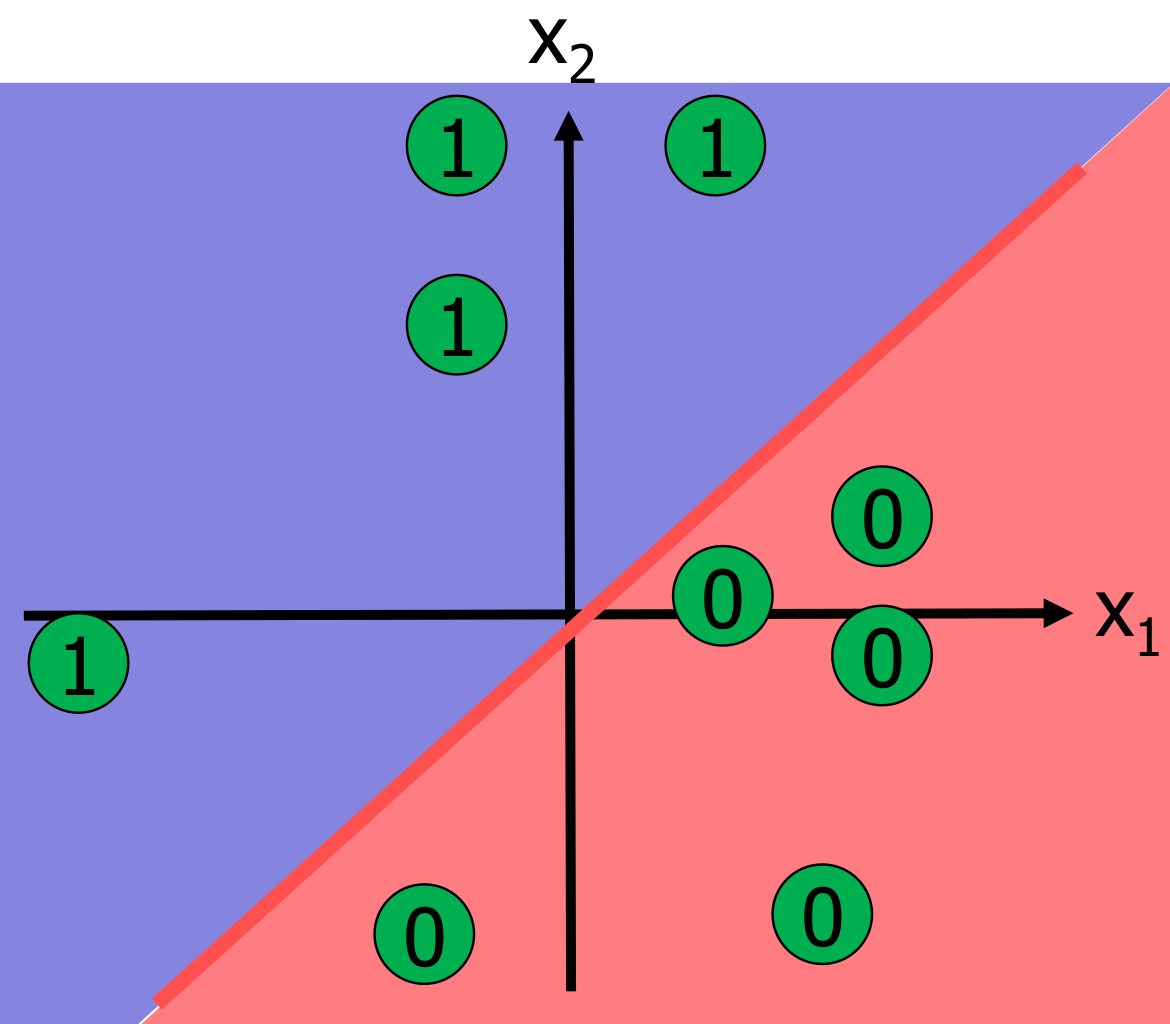
\includegraphics[height=4.5cm,keepaspectratio]{pics/PCT_regions}};
        \node<1>[below of=theta,yshift=-19mm] {\small MVA output $y=0~or~1$};

        \node<2>[inner sep=0pt] (actpic) at (0,0)
            {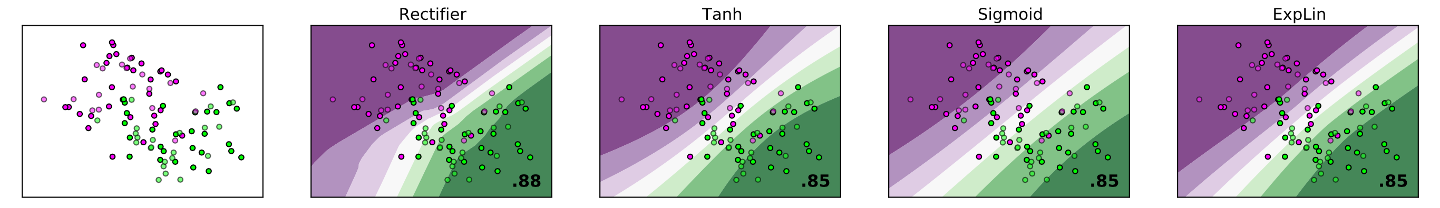
\includegraphics[height=1.5cm,keepaspectratio]{pics/plot_activation.png}};        

        \node<2>[below=1cm of actpic,inner sep=0pt] (dist) {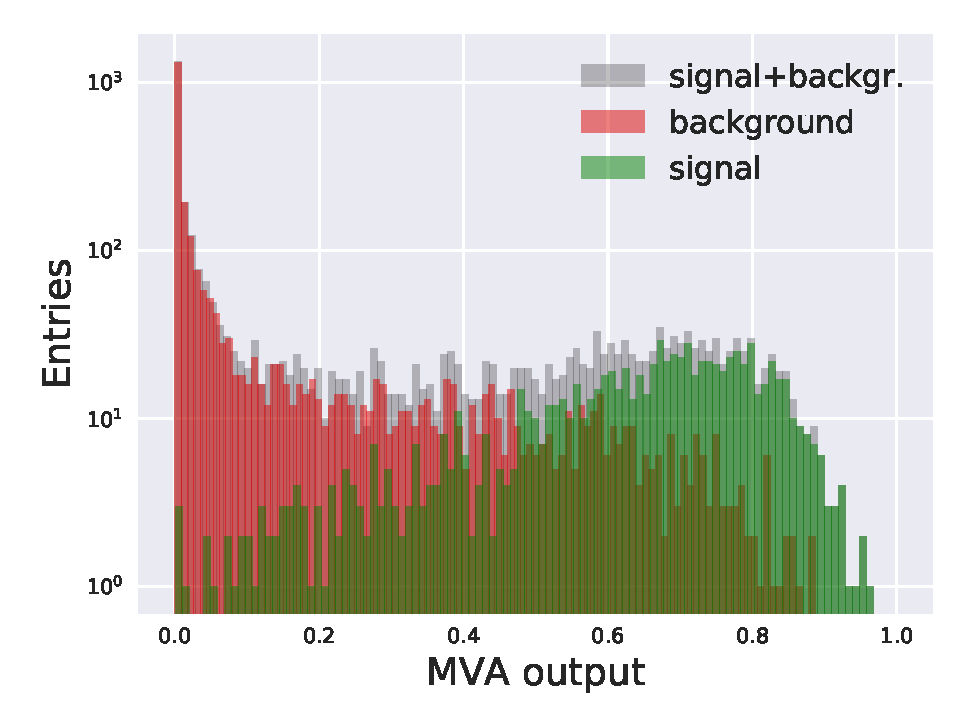
\includegraphics[height=4.1cm,keepaspectratio]{pics/MVAoutput_distr_train_log.pdf}};
        \node<2>[right of=dist,xshift=30mm,text width=2cm] {\small MVA output $y\in(0,1)$};
        \draw<2>[->, color=black, ultra thick] (2,-0.8) to [out=270,in=90] (dist.north);
    \end{tikzpicture}
     

\end{frame}

% -----------------------------------------------

\begin{frame}
    \frametitle{Improving linear methods}
    \begin{block}{Kernel trick}
        Map data to a higher dimensional space where linear hyperplane can again be found
    \end{block}
    \begin{columns}[T] % align columns
        \begin{column}{.48\textwidth}
            \raggedleft\includegraphics<2->[height=4.3cm,keepaspectratio]{pics/kernel_trick_r2.png}%            
        \end{column}
        \begin{column}{.48\textwidth}
            \raggedright\includegraphics<3->[height=4.3cm,keepaspectratio]{pics/kernel_trick_r3.png}%            
        \end{column}
    \end{columns}
    
\end{frame}

% -----------------------------------------------

\subsection{Non-linear cuts}
% \begin{frame}
%     \frametitle{Non-linear models}
%     \begin{block}{Assumtion}
%         Take \emph{kernel trick} idea: map inputs $\boldsymbol{x} = (x_{1},\dots x_{n})$ to higher dimensional space $\mathbb{R}^{m}$ with $m~>~n$
%         where linear seperation is possible:
%         \vspace*{3mm}
%         \begin{align*} 
%               % y: \mathbb{R}^{n} \to \mathbb{R}^{m} \to \mathbb{R}~|~\boldsymbol{x} \mapsto y  &= 
%               %   \sigma (w^{(2)}_{0} + \boldsymbol{w^{(2)}} \cdot \sigma (w^{(1)}_{0} + \boldsymbol{w^{(1)}} \cdot \boldsymbol{x}) )\\ 
%               % y: \mathbb{R}^{n} \to \mathbb{R}^{m}  &=  \sigma (w^{(2)}_{0} + \boldsymbol{w^{(2)}} \cdot \sigma (w^{(1)}_{0} + \boldsymbol{w^{(1)}} \cdot \boldsymbol{x}) )\\ 
%             y: \mathbb{R}^{n} \to \mathbb{R}^{m} \to \mathbb{R} &= \sigma \left( w_{0}^{2} + \sum_{i=1}^{m} \left[ w_{i}^{(2)} + \sigma \left( w_{0,i}^{(1)} + \sum_{k=1}^{n} w_{k,i}^{(1)}~x_{k} \right) \right] \right)\\
%             &=  \sigma \left[ w^{(2)}_{0} + \boldsymbol{w}^{(2)} \cdot \sigma(\boldsymbol{w}^{(1)}_{0}+ \boldsymbol{W}^{(1)} \cdot \boldsymbol{x})\right]
%         \end{align*}
%         \vspace*{3mm}
%         $\to$ $m$ \emph{single layer perceptrons}
%     \end{block}
% \end{frame} 

% -----------------------------------------------

\begin{frame}
    \frametitle{Non-linear models}
    \centering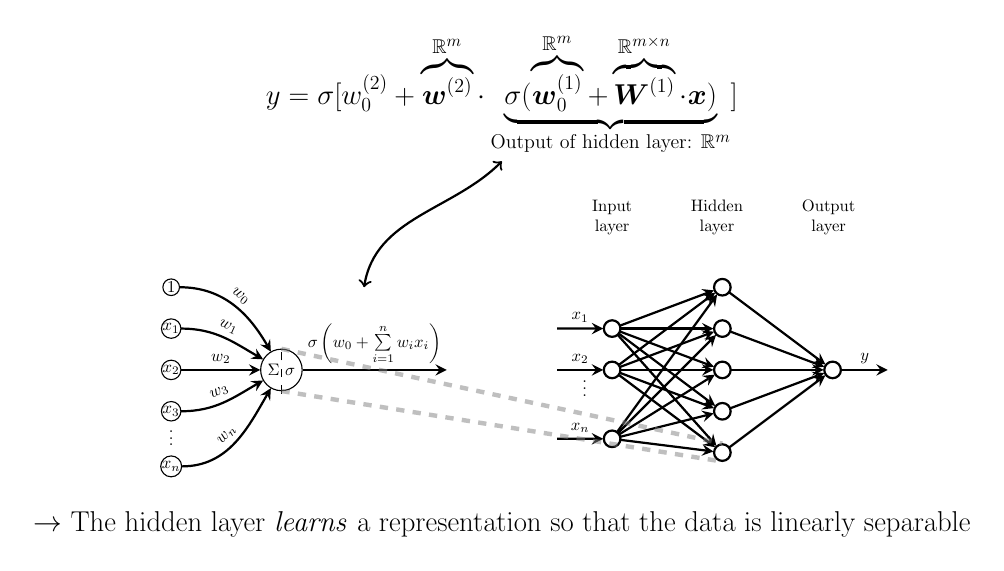
\begin{tikzpicture}[scale=0.7, every node/.style={scale=0.6}]

        \node[draw,circle,minimum size=25pt,inner sep=0pt] (x) at (0,0) {$\Sigma$ $\sigma$};
        \node[align=center] (formula) at (4, 5){\LARGE$y = \sigma [  w^{(2)}_{0} + \overbrace{ \boldsymbol{w}^{(2)} }^{\mathbb{R}^{m}} \cdot \underbrace{\sigma(\overbrace{\boldsymbol{w}^{(1)}_{0}}^{\mathbb{R}^{m}}+ \overbrace{\boldsymbol{W}^{(1)}}^{\mathbb{R}^{m\times n}} \cdot \boldsymbol{x})}_{\text{Output of hidden layer:}~\mathbb{R}^{m}}]$};

        \node[inputNode] (x0) at (-2, 1.5) {$\tiny 1$};
        \node[inputNode] (x1) at (-2, 0.75) {$\tiny x_1$};
        \node[inputNode] (x2) at (-2, 0) {$\tiny x_2$};
        \node[inputNode] (x3) at (-2, -0.75) {$\tiny x_3$};
        \node[inputNode] (xn) at (-2, -1.75) {$\tiny x_n$};

        \draw[stateTransition] (x0) to[out=0,in=120] node [midway, sloped, above] {$w_0$} (x);
        \draw[stateTransition] (x1) to[out=0,in=150] node [midway, sloped, above] {$w_1$} (x);
        \draw[stateTransition] (x2) to[out=0,in=180] node [midway, sloped, above] {$w_2$} (x);
        \draw[stateTransition] (x3) to[out=0,in=210] node [midway, sloped, above] {$w_3$} (x);
        \draw[stateTransition] (xn) to[out=0,in=240] node [midway, sloped, above] {$w_n$} (x);
        \draw[stateTransition] (x) -- (3,0) node [midway,above] {$\sigma\left(w_0 + \sum\limits_{i=1}^{n}{w_ix_i}\right)$};
        \draw[dashed] (0,-0.43) -- (0,0.43);
        \node (dots) at (-2, -1.15) {$\vdots$};

        \draw[<->, color=black, thick] (1.5, 1.5) to [out=90,in=225, xshift=2mm] (formula.south);

        \pause
        \node[inputNode, thick] (i1) at (6, 0.75) {};
        \node[inputNode, thick] (i2) at (6, 0) {};
        \node[inputNode, thick] (i3) at (6, -1.25) {};
        
        \node[inputNode, thick] (h1) at (8, 1.5) {};
        \node[inputNode, thick] (h2) at (8, 0.75) {};
        \node[inputNode, thick] (h3) at (8, 0) {};
        \node[inputNode, thick] (h4) at (8, -0.75) {};
        \node[inputNode, thick] (h5) at (8, -1.5) {};
        
        \node[inputNode, thick] (o1) at (10, 0) {};
        
        \draw[stateTransition] (5, 0.75) -- node[above] {$x_{1}$} (i1);
        \draw[stateTransition] (5, 0) -- node[above] {$x_{2}$} (i2);
        \draw[stateTransition] (5, -1.25) -- node[above] {$x_{n}$} (i3);
        \node (dots) at (5.5, -0.25) {$\vdots$};
        
        \draw[stateTransition] (i1) -- (h1);
        \draw[stateTransition] (i1) -- (h2);
        \draw[stateTransition] (i1) -- (h3);
        \draw[stateTransition] (i1) -- (h4);
        \draw[stateTransition] (i1) -- (h5);
        \draw[stateTransition] (i2) -- (h1);
        \draw[stateTransition] (i2) -- (h2);
        \draw[stateTransition] (i2) -- (h3);
        \draw[stateTransition] (i2) -- (h4);
        \draw[stateTransition] (i2) -- (h5);
        \draw[stateTransition] (i3) -- (h1);
        \draw[stateTransition] (i3) -- (h2);
        \draw[stateTransition] (i3) -- (h3);
        \draw[stateTransition] (i3) -- (h4);
        \draw[stateTransition] (i3) -- (h5);
        
        \draw[stateTransition] (h1) -- (o1);
        \draw[stateTransition] (h2) -- (o1);
        \draw[stateTransition] (h3) -- (o1);
        \draw[stateTransition] (h4) -- (o1);
        \draw[stateTransition] (h5) -- (o1);
        
        \node[above=of i1, align=center] (l1) {Input \\ layer};
        \node[right=1.7em of l1, align=center] (l2) {Hidden \\ layer};
        \node[right=1.7em of l2, align=center] (l3) {Output \\ layer};
        
        \draw[stateTransition] (o1) -- node[above] {$y$} (11, 0);
        
        \path[dashed, double, ultra thick, gray, opacity=0.5] (x.north) edge[bend left=0] (h5.north);
        \path[dashed, double, ultra thick, gray, opacity=0.5] (x.south) edge[bend right=0] (h5.south);

        \pause
        \node[align=center] (txt) at (4, -2.8) {\LARGE$\to$ The hidden layer \emph{learns} a representation so that the data is linearly separable};
    \end{tikzpicture}

\end{frame}

% -----------------------------------------------

% \begin{frame}
%     \frametitle{Visualising the hidden layer}
%     \begin{block}{Effects of adding a hidden layer}
%         Input vector $\boldsymbol{x}$ undergoes \emph{linear transformation} by multiplication with weight matrix $\boldsymbol{W}$. The bias term $\boldsymbol{w}_{0}$ causes a \emph{translation}.\\
%     \end{block}
%     \vspace*{5mm}
%     \centering\begin{tikzpicture}
%         \node<1>[align=center] (formula) at (1, 2){$y = \sigma [  w^{(2)}_{0} + \boldsymbol{w}^{(2)} \cdot \underbrace{\sigma(\boldsymbol{w}^{(1)}_{0} + \boldsymbol{W}^{(1)}
%             \cdot \boldsymbol{x})}_{\mathbb{\boldsymbol{\tilde{x}}}}]$};

%         \node<2->[align=center] (formula) at (1, 2){$\boldsymbol{\tilde{x}} = \sigma(\boldsymbol{w}^{(1)}_{0}+ \boldsymbol{W}^{(1)} \cdot \boldsymbol{x})~\text{ with \emph{e.g.}}~\boldsymbol{W}= \begin{pmatrix} w_{1}^{1} & w_{1}^{2} \\ w_{2}^{1} & w_{2}^{2} \end{pmatrix} $ };

%         \pause
%         \node[inputNode, thick] (i1) at (0, 1) {};
%         \node[inputNode, thick] (i2) at (0, -1) {};
        
%         \node[inputNode, thick] (h1) at (2, 1) {};
%         \node[inputNode, thick] (h2) at (2, -1) {};

%         \draw[stateTransition] (-1, 1) -- node[left, xshift=-4mm] {$x_{1}$} (i1);
%         \draw[stateTransition] (-1, -1) -- node[left,xshift=-4mm] {$x_{2}$} (i2);
       
%         \draw[stateTransition] (i1) -- node[midway,fill=white] {\tiny$w_{1}^{1}$} (h1);
%         \draw[stateTransition] (i1) -- node[midway,fill=white, xshift=-4mm, yshift=4mm] {\tiny$w_{1}^{2}$} (h2);

%         \draw[stateTransition] (i2) -- node[midway,fill=white, xshift=-4mm, yshift=-4mm] {\tiny$w_{2}^{1}$} (h1);
%         \draw[stateTransition] (i2) -- node[midway,fill=white] {\tiny$w_{2}^{2}$} (h2);

%         \draw[stateTransition] (h1) -- node[right, xshift=4mm] {$x_{1}\textprime$} (3, 1);
%         \draw[stateTransition] (h2) -- node[right, xshift=4mm] {$x_{2}\textprime$} (3, -1);

%         % \path[dashed, double, ultra thick, gray, opacity=0.5] (x.north) edge[bend left=0] (h5.north);
%         % \path[dashed, double, ultra thick, gray, opacity=0.5] (x.south) edge[bend right=0] (h5.south);
%     \end{tikzpicture}
% \end{frame}

% -----------------------------------------------

\begin{frame}
    \frametitle{Visualising the hidden layer}
    \begin{columns}[T] % align columns        
        \begin{column}{.48\textwidth}
            \vspace*{-5mm}
            \begin{enumerate}
                \item<2-> Linear transformation:~$\boldsymbol{W}\boldsymbol{x}$\\
                \item<3-> Translation:~$\boldsymbol{w}_{0}$\\
                \item<4-> Non-linear activation:~$\sigma$
            \end{enumerate}
            \vspace*{2mm}
            \begin{tikzpicture}
                \node<1-4>[align=center] (formula) at (1, 1.8){$\boldsymbol{\tilde{x}} = \only<1>{\boldsymbol{x}} \only<4>{\sigma}\only<2-4>{(}\only<3-4>{\boldsymbol{w}^{(1)}_{0}+} \only<2-4>{\boldsymbol{W}^{(1)} \cdot \boldsymbol{x})}$\\ };
                \node<5->[align=center] (formula) at (1, 1.8){$y = \sigma(w^{(2)}_{0} + \boldsymbol{w}^{(2)} \cdot \boldsymbol{\tilde{x}})$\\ };

                \pause
                \node[inputNode, thick] (i1) at (0, 1) {};
                \node[inputNode, thick] (i2) at (0, -1) {};
                
                \node[inputNode, thick] (h1) at (2, 1) {};
                \node[inputNode, thick] (h2) at (2, -1) {};

                \draw[stateTransition] (-1, 1) -- node[left, xshift=-4mm] {$x_{1}$} (i1);
                \draw[stateTransition] (-1, -1) -- node[left,xshift=-4mm] {$x_{2}$} (i2);
               
                \draw[stateTransition] (i1) -- node[midway,fill=white] {\tiny$w_{1}^{1}$} (h1);
                \draw[stateTransition] (i1) -- node[midway,fill=white, xshift=-4mm, yshift=4mm] {\tiny$w_{1}^{2}$} (h2);

                \draw[stateTransition] (i2) -- node[midway,fill=white, xshift=-4mm, yshift=-4mm] {\tiny$w_{2}^{1}$} (h1);
                \draw[stateTransition] (i2) -- node[midway,fill=white] {\tiny$w_{2}^{2}$} (h2);

                \draw<1-3>[stateTransition] (h1) -- node[right, xshift=4mm] {$x_{1}\textprime$} (3, 1);
                \draw<1-3>[stateTransition] (h2) -- node[right, xshift=4mm] {$x_{2}\textprime$} (3, -1);

                \node<3->[inputNode, thick] (b) at (0, -2) {1};
                \draw<3->[stateTransition] (b) -- node[midway,fill=white, xshift=-7mm, yshift=-10mm] {\tiny$w_{0}^{1}$} (h1);
                \draw<3->[stateTransition] (b) -- node[midway,fill=white] {\tiny$w_{0}^{2}$} (h2);

                \draw<4>[stateTransition] (h1) -- node[right, xshift=4mm] {$\sigma(x_{1}\textprime)$} (3, 1);
                \draw<4>[stateTransition] (h2) -- node[right, xshift=4mm] {$\sigma(x_{2}\textprime)$} (3, -1);

                \node<5->[inputNode, thick] (o) at (3, 0) {};
                \draw<5->[stateTransition] (h1) -- (o) {};
                \draw<5->[stateTransition] (h2) -- (o) {};
                \draw<5->[stateTransition] (o) -- node[above] {$y$} (4,0);
 
            \end{tikzpicture}
        \end{column}
        \hfill%
        \begin{column}{.48\textwidth}
            \vspace*{8mm}
            \raggedright\includegraphics<1>[height=4.8cm,keepaspectratio]{pics/MLP_featspace_inital_state}%            
            \raggedright\includegraphics<2>[height=4.8cm,keepaspectratio]{pics/MLP_featspace_matmul}%            
            \raggedright\includegraphics<3>[height=4.8cm,keepaspectratio]{pics/MLP_featspace_translation}%            
            \raggedright\includegraphics<4>[height=4.8cm,keepaspectratio]{pics/MLP_featspace_final_state}%            
            \raggedright\includegraphics<5>[height=4.8cm,keepaspectratio]{pics/MLP_featspace_final_state_cut}%            
        \end{column}% 
    \end{columns}

\end{frame}

% % -----------------------------------------------
\begin{frame}
    \frametitle{Update weights via back-propergation}
    \begin{block}{Backpropergation}
        Adapt weights by going backwards in the network
        \begin{itemize}
            \item<1-> Initialize weigts
            \item<2-> Evaluate $y_{predict} = f(\boldsymbol{x})$ and calculate $\Delta = (y_{true} - y_{predict})$
            \item<3-> Update weights: Weight adaption often denoted via loss $L = L(y_{true},\boldsymbol{w}^{(1)},\boldsymbol{W}^{(2)})$
        \end{itemize}
    \end{block} 
    \vspace*{3mm}
    \centering\begin{tikzpicture}
        \node<4->[inner sep=0pt] (loss) at (0,0)
            {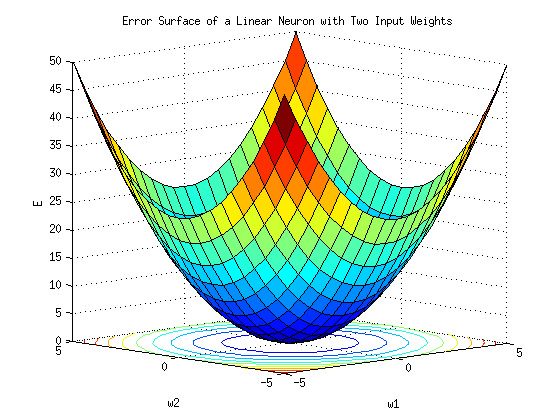
\includegraphics[height=3.1cm,keepaspectratio]{pics/loss_func}};
        \node<4->[right=of loss, xshift=-2mm,yshift=0mm] (txt) {Minimize loss~$\to$~find best fit};
        \draw<4->[->,red,thick] (txt.west) to [out=180, in=45] (0,-0.9);
    \end{tikzpicture}
\end{frame}

% -----------------------------------------------

% \begin{frame}
%     \frametitle{Quantify MVA output}
%     \begin{block}{Evaluate classifier performance}
%         \begin{itemize}
%             \item Compare predicted class labels with the true ones $\to$ confusion matrix
%        \end{itemize}
%     \end{block}
%     \vspace*{4mm}
%     \centering\includegraphics<1>[height=4.8cm,keepaspectratio]{pics/Confusion_matrix}%            
% \end{frame}

% % -----------------------------------------------

\begin{frame}
    \frametitle{Quantify MVA output}
    \begin{block}{Evaluate classifier performance}
        \begin{itemize}
            \item ROC curve: continuously scan y \& plot background acceptance (FPR) vs. signal efficiency (TPR)
                
        \end{itemize}
    \end{block}
    \vspace*{2mm}
    \centering\begin{tikzpicture}
        \node[inner sep=0pt] (roc) at (0,0)
            {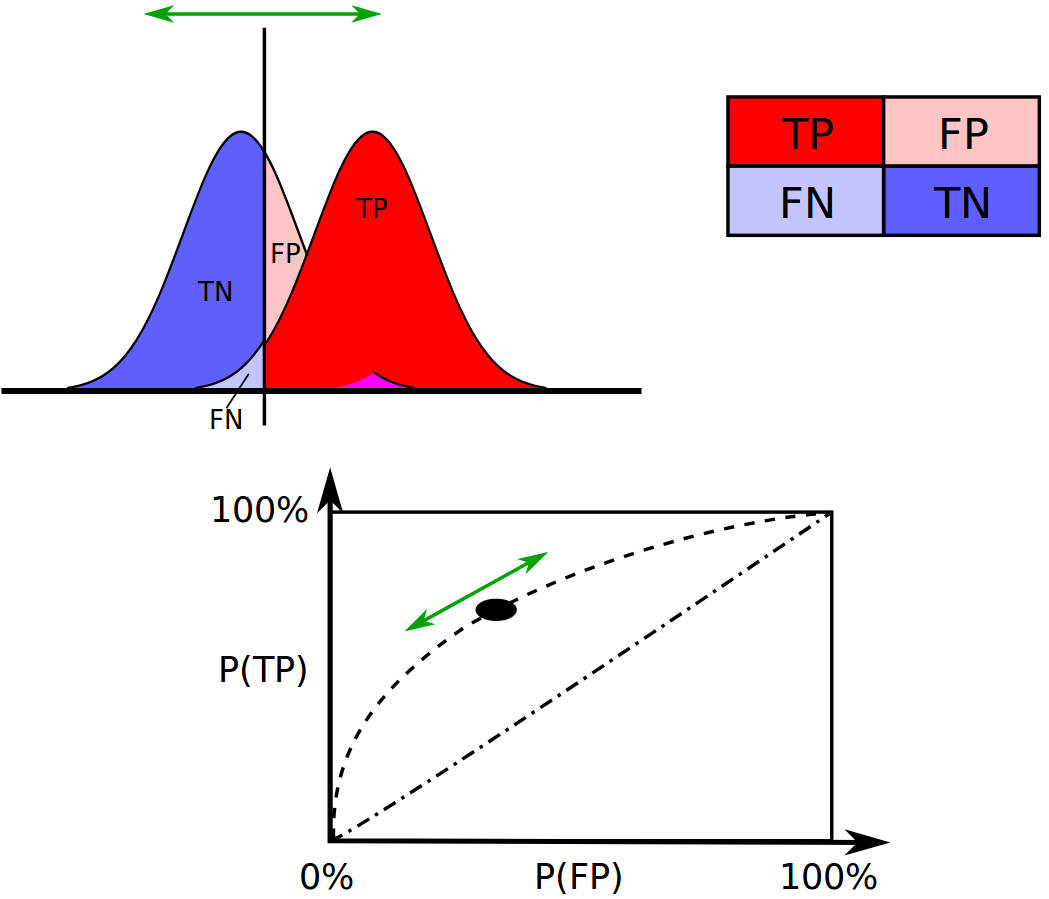
\includegraphics[height=3.8cm,keepaspectratio]{pics/roc_curve}};
        % \draw[->, color=black, ultra thick] (2,-0.8) to [out=270,in=90] (roc.north);
        \node[align=center] (formula) at (5, 0) {\small$\text{FPR = FP/(FP+TN)}$};
        \node[align=center, below=of formula,yshift=9mm] (formula2) {\small$\text{TPR = TP/ (TP + FN)}$};
        \node[align=center, below=of roc,yshift=9mm,xshift=20mm,text width=0.8\paperwidth] (auc) {\footnotesize ROC-AUC: probability that classifier ranks randomly chosen positive sample higher than randomly chosen negative one};
    \end{tikzpicture}
\end{frame}

% % -----------------------------------------------

\begin{frame}
    \frametitle{Bias-variance tradeof}
    \begin{itemize}
        \item Small variance: Classifiers with low degrees of freedom are less prone to statistical fluctuations\\$\to$~different training samples result in similar classification boundaries 
        \item However: if data contain features that a model with few degrees of freedom cannot describe, a bias is introduced
    \end{itemize}
    \vspace*{3mm}
    \centering\includegraphics<1>[height=3.0cm,keepaspectratio]{pics/Overfitting}%
    % \centering\includegraphics<2>[height=3.8cm,keepaspectratio]{pics/overfitting_2}%
\end{frame}


% -----------------------------------------------

% \begin{frame}
%     \frametitle{Getting started}
%     add piece of code \& show how easy it is
% \end{frame}


% -----------------------------------------------

{\setbeamercolor{background canvas}{bg=red!20}
\begin{frame}
    \frametitle{MVA applied to CEP data}
    In order to reduce the main background component - \textbf{feed down} - ML is applied on simulated data.\\
    \vspace*{5mm}
    \centering\begin{tikzpicture}
        \node[inner sep=0pt] (cov) at (0,0) {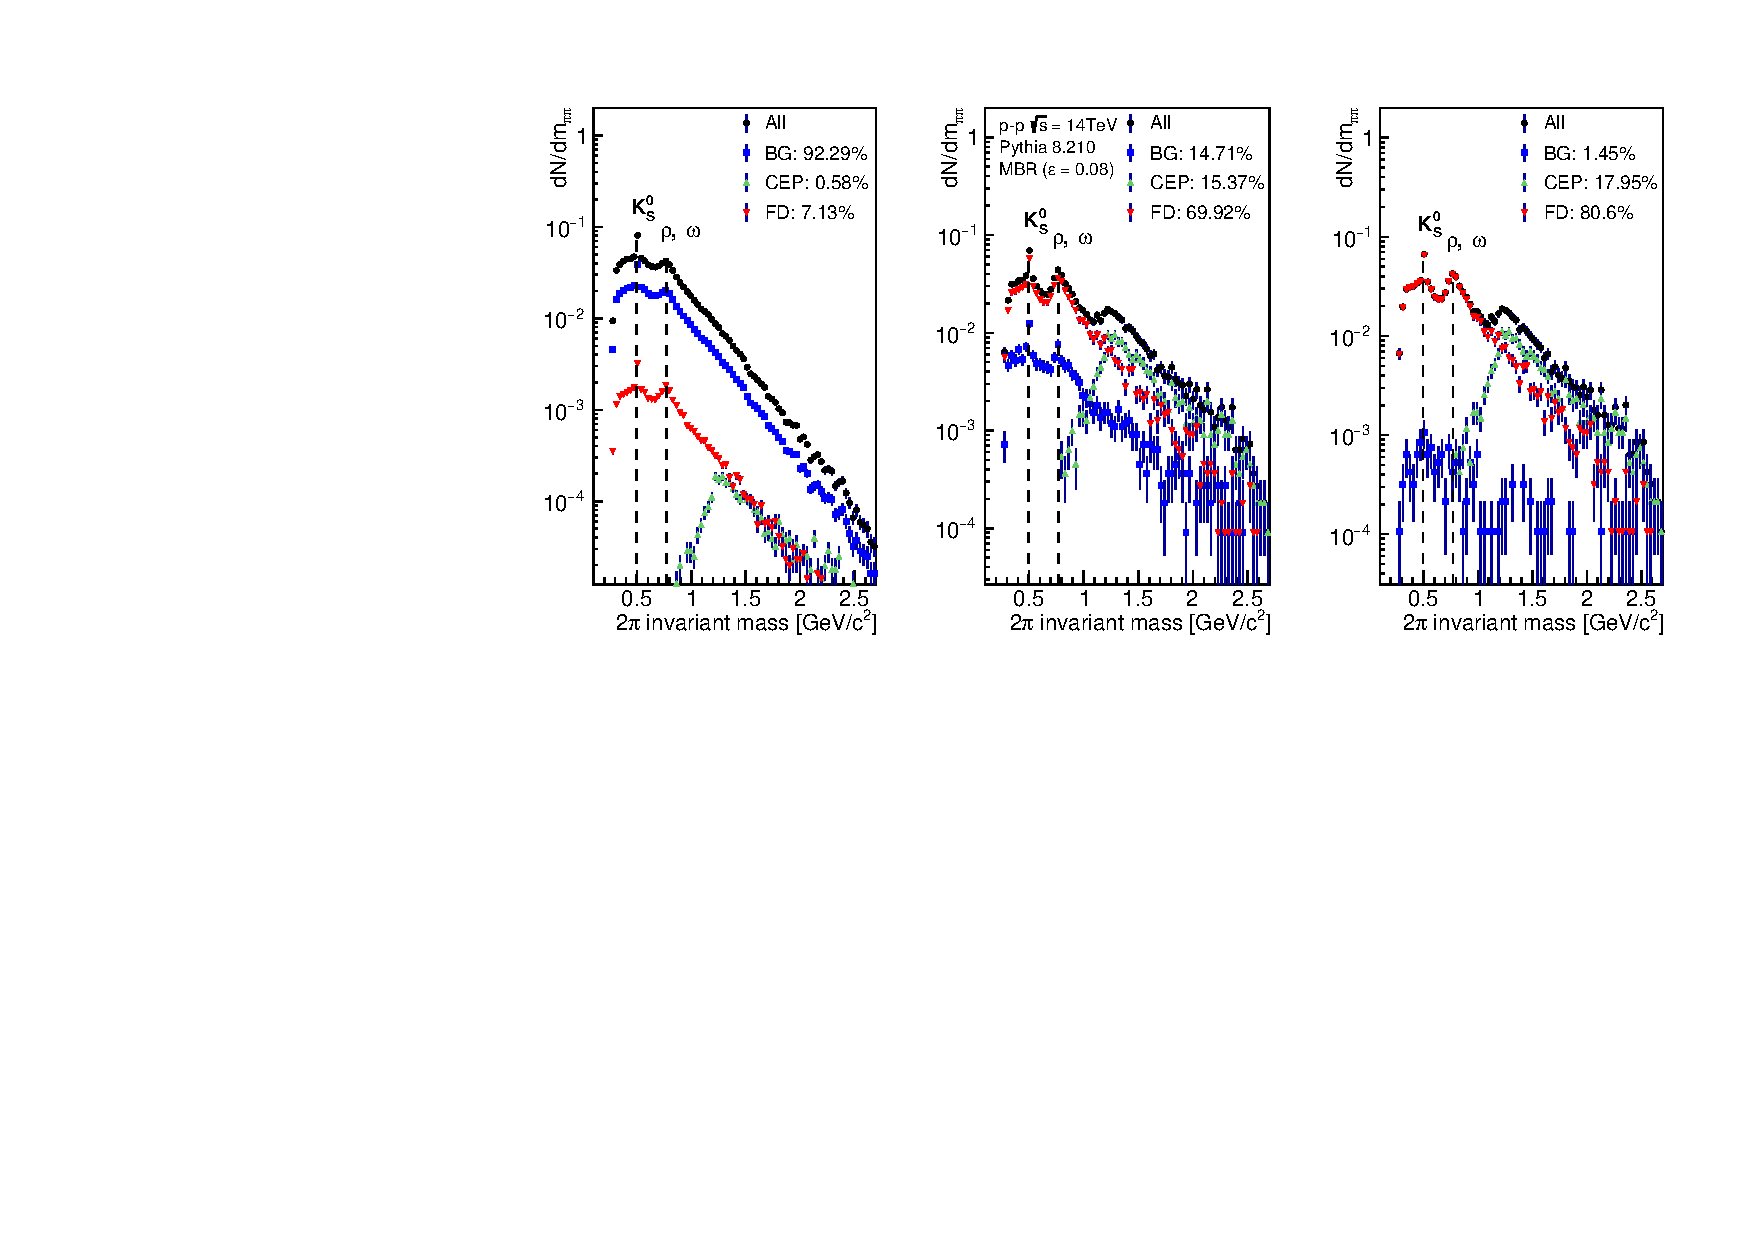
\includegraphics[height=5.1cm,keepaspectratio]{pics/detected_simulated_newLabels}};
        \node[above=of cov, yshift=-15mm] (txt) {$\to$~increasing~$\Delta\eta$};

        % \draw[->, thick] (det) -- (cov);

        % \node[align = center, above = of det, yshift=-9mm] {\small CEP event};
        % \node[align = center, above = of cov, yshift=-9mm] {\small $\eta$ coverage};

        % \node<2-> (rectbarrel) at (3.35,0.18) [color=red,rectangle, dashed, minimum height=28mm,minimum width=8mm,draw, thick] {};

        % \node<3-> (rectbarrel1) at (4.6,0.18) [rectangle, dashed, minimum height=28mm,minimum width=16mm,draw, thick] {};
        % \node<3-> (rectbarrel2) at (2.1,0.18) [rectangle, dashed, minimum height=28mm,minimum width=16mm,draw, thick] {};

        % \node (rectroot) at (0,0) [rectangle, dashed, color=red, minimum height=2cm,minimum width=3cm,draw, thick] {};
        % \node (rootbottom) [below=1mm of rectroot, color=red]  {Root node};

        % \node[inner sep=0pt] (nd) at (0,-4) {\[includegraphicsheight=1.1cm,keepaspectratio]{pics/ND_eta}};
        % \node[align = center, below = of nd, yshift=9mm] {\small Non-diffractive};
        % \node[below=of nd, node distance=0cm, yshift=10mm, xshift=11mm] {\small$\eta$};
        % \node[left=of nd, node distance=0cm, rotate=0, anchor=center,yshift=4mm, xshift=8mm] {\small$\phi$};
    \end{tikzpicture}
\end{frame}
}


\section{Results \& Conclusion}

\begin{frame}
    \frametitle{Neural network structure}
    \centering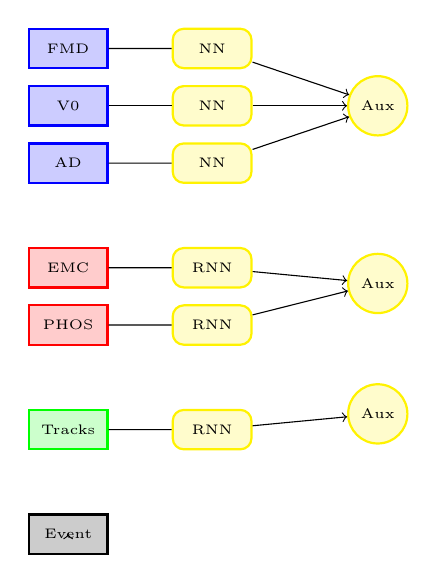
\begin{tikzpicture}
        \node (rectFMD) at (0,0) [text=black,draw=blue, fill=blue!20,rectangle, minimum height=5mm,minimum width=10mm,draw, thick] {\tiny FMD};
        \node[right=of rectFMD,xshift=-2mm] (rectNNFMD) [text=black,draw=yellow,fill=yellow!20,rectangle, minimum height=5mm,minimum width=10mm,draw, thick,rounded corners] {\tiny NN};

        \node[below=of rectFMD,yshift=8mm] (rectV0) [text=black,draw=blue,fill=blue!20,rectangle, minimum height=5mm,minimum width=10mm,draw, thick] {\tiny V0};
        \node[right=of rectV0,xshift=-2mm] (rectNNV0) [text=black,draw=yellow,fill=yellow!20,rectangle,minimum height=5mm,minimum width=10mm,draw, thick,rounded corners] {\tiny NN};
        \node[right=of rectNNV0,xshift=2mm] (VetoAux) [draw=yellow,fill=yellow!20,circle,draw, thick,minimum size=6mm] {\tiny Aux};
        \draw[->] (rectV0) -- (rectNNV0) -- (VetoAux);
        \draw[->] (rectFMD) -- (rectNNFMD) -- ([xshift=2mm]rectNNFMD) -- (VetoAux);

        \node[below=of rectV0,yshift=8mm] (rectAD) [text=black,draw=blue,fill=blue!20,rectangle, minimum height=5mm,minimum width=10mm,draw, thick] {\tiny AD};
        \node[right=of rectAD,xshift=-2mm] (rectNNad) [text=black,draw=yellow,fill=yellow!20,rectangle, minimum height=5mm,minimum width=10mm,draw, thick,rounded corners] {\tiny NN};
        \draw[->] (rectAD) -- (rectNNad) -- ([xshift=2mm]rectNNad) -- (VetoAux);

        \node[below=of rectAD,yshift=2mm] (rectEMC) [text=black,draw=red,fill=red!20,rectangle, minimum height=5mm,minimum width=10mm,draw, thick] {\tiny EMC};
        \node[right=of rectEMC,xshift=-2mm] (rectRNNemc) [text=black,draw=yellow,fill=yellow!20,rectangle, minimum height=5mm,minimum width=10mm,draw, thick,rounded corners] {\tiny RNN};
        \node[right=of rectRNNemc,xshift=2mm,yshift=-2mm] (VetoAuxCalo) [draw=yellow,fill=yellow!20,circle,draw, thick,minimum size=6mm] {\tiny Aux};
        \draw[->] (rectEMC) -- (rectRNNemc) -- (VetoAuxCalo);

        \node[below=of rectEMC,yshift=8mm] (rectPHOS) [text=black,draw=red,fill=red!20,rectangle, minimum height=5mm,minimum width=10mm,draw, thick] {\tiny PHOS};
        \node[right=of rectPHOS,xshift=-2mm] (rectRNNphos) [text=black,draw=yellow,fill=yellow!20,rectangle, minimum height=5mm,minimum width=10mm,draw, thick,rounded corners] {\tiny RNN};
        \draw[->] (rectPHOS) -- (rectRNNphos) -- (VetoAuxCalo);

        \node[below=of rectPHOS,yshift=2mm] (rectTrack) [text=black,draw=green,fill=green!20,rectangle, minimum height=5mm,minimum width=10mm,draw, thick] {\tiny Tracks};
        \node[right=of rectTrack,xshift=-2mm] (rectRNNtrack) [text=black,draw=yellow,fill=yellow!20,rectangle, minimum height=5mm,minimum width=10mm,draw, thick,rounded corners] {\tiny RNN};
        \node[right=of rectRNNtrack,xshift=2mm,yshift=2mm] (VetoAuxTrack) [draw=yellow,fill=yellow!20,circle,draw, thick,minimum size=6mm] {\tiny Aux};
        \draw[->] (rectTrack) -- (rectRNNtrack) -- (VetoAuxTrack);

        \node[below=of rectTrack,yshift=2mm] (rectEvent) [text=black,draw=black,fill=black!20,rectangle, minimum height=5mm,minimum width=10mm,draw, thick] {\tiny Event};
        \draw[->] (rectEvent) -- ([xshift=4mm]rectEvent);


    \end{tikzpicture}
     
\end{frame}

\begin{frame}
    \frametitle{Results}
    \centering\begin{tikzpicture}
        \node[inner sep=0pt] (f1) at (0,0)
            {\includegraphics[height=20mm,keepaspectratio]{pics/pt}};
        \node[inner sep=0pt, below=of f1,yshift=9mm] (f2)
            {\includegraphics[height=20mm,keepaspectratio]{pics/z_impact}};
        \node[inner sep=0pt, below=of f2,yshift=9mm] (dots)
            {\LARGE$\vdots$};
        \node[inner sep=0pt, below=of dots,yshift=9mm] (fn)
            {\includegraphics[height=20mm,keepaspectratio]{pics/pid_bayes_proba_pion}};
        \draw [decorate,decoration={brace,amplitude=15pt},xshift=5mm,yshift=0pt]
            (f1.north east) -- (fn.south east) node [black,midway,xshift=15mm] 
            {$\mathbb{R}^{n}\to\mathbb{R}$};
        \node<1>[inner sep=0pt, right=of dots,yshift=9mm,xshift=30mm] (output)
            {\includegraphics[height=45mm,keepaspectratio]{pics/MVAoutput_distr_train_log}};

        % ROC curves
        % train
        % \node<2>[inner sep=0pt, right=of dots,yshift=9mm,xshift=30mm] (roctrain)
        %     {\includegraphics[height=45mm,keepaspectratio]{pics/roc_curve_train}};
        % \node<2>[inner sep=0pt, above=of roctrain,yshift=-9mm] (roctrainTXT)
        %     {\footnotesize ROC train};
        % % test
        % \node<3>[inner sep=0pt, right=of dots,yshift=9mm,xshift=30mm] (roctest)
        %     {\includegraphics[height=45mm,keepaspectratio]{pics/roc_curve_test}};
        % \node<3>[inner sep=0pt, above=of roctest,yshift=-9mm] (roctestTXT)
        %     {\footnotesize ROC test};

        % %significance
        % \node<4>[inner sep=0pt, right=of dots,yshift=9mm,xshift=30mm] (sign)
        %     {\includegraphics[height=45mm,keepaspectratio]{pics/significance_vs_MVAcut}};
        % \node<4>[inner sep=0pt, above=of sign,yshift=-9mm] (sigTXT)
        %     {\footnotesize Significance $S=N_{sig}/\sqrt{N_{sig}+N_{BG}}$};

        % % inv mass
        % \node<5>[inner sep=0pt, right=of dots,yshift=25mm,xshift=30mm] (invar1)
        %     {\includegraphics[height=30mm,keepaspectratio]{pics/noV0_invar_mass_plot}};
        % \node<5>[inner sep=0pt, above=of invar1,yshift=-9mm] (invar1TXT)
        %     {\footnotesize no MVA cut};
        % \node<5>[inner sep=0pt, right=of dots,yshift=-7mm,xshift=30mm] (invar2)
        %     {\includegraphics[height=30mm,keepaspectratio]{pics/invar_mass_plot}};
        % \node<5>[inner sep=0pt, below=of invar2,yshift=9mm] (invar2TXT)
        %     {\footnotesize with MVA cut};
      \end{tikzpicture}
\end{frame}

% -----------------------------------------------

\begin{frame}
    \frametitle{Results}
    ROC curve\\
    \vspace*{5mm}
    \centering\begin{tikzpicture}
        \node<1-2>[inner sep=0pt] (output) at (0,0)
            {\includegraphics[height=40mm,keepaspectratio]{pics/MVAoutput_distr_train_log}};
        \node<1-2>[inner sep=0pt, above=of output,yshift=-9mm] (trainTXT)
            {\footnotesize Training data};

        % ROC curves
        % train
        \node<2>[inner sep=0pt, right=of output,yshift=3mm,xshift=-5mm] (roctrain)
            {\includegraphics[height=42mm,keepaspectratio]{pics/roc_curve_train}};
        \node<2>[inner sep=0pt, above=of roctrain,yshift=-9mm] (roctrainTXT)
            {\footnotesize ROC train};
        % test
        \node<3>[inner sep=0pt] (output) at (0,0)
            {\includegraphics[height=40mm,keepaspectratio]{pics/MVAoutput_distr_test_log}};        
        \node<3>[inner sep=0pt, above=of output,yshift=-9mm] (testTXT)
            {\footnotesize Test data};

        \node<3>[inner sep=0pt, right=of output,yshift=3mm,xshift=-5mm] (roctest)
            {\includegraphics[height=42mm,keepaspectratio]{pics/roc_curve_test}};
        \node<3>[inner sep=0pt, above=of roctest,yshift=-9mm] (roctestTXT)
            {\footnotesize ROC test};

      \end{tikzpicture}
\end{frame}

% -----------------------------------------------

\begin{frame}
    \frametitle{Results}
    To find the optimal cut on MVA output we evaluate significance along $y$\\
    \vspace*{5mm}
    \centering\begin{tikzpicture}
        \node<1->[inner sep=0pt] (output) at (0,0)
            {\includegraphics[height=40mm,keepaspectratio]{pics/MVAoutput_distr_train_log}};

        %significance
        \node<2->[inner sep=0pt, right=of output,yshift=0mm,xshift=-7mm] (sign)
            {\includegraphics[height=40mm,keepaspectratio]{pics/significance_vs_MVAcut}};
        \node<2->[inner sep=0pt, below=of sign,yshift=8mm,xshift=-25mm] (sigTXT)
            {\footnotesize Significance $S=\frac{N_{sig}}{\sqrt{N_{sig}+N_{BG}}}$ };

        \draw<3->[color=red, ultra thick, dashed] (-0.16, -1.35) -- (-0.16,1.2);

      \end{tikzpicture}
\end{frame}

% -----------------------------------------------

\begin{frame}
    \frametitle{Results}
    \centering\begin{tikzpicture}
        \node<1->[inner sep=0pt] (output) at (0,0)
            {\includegraphics[height=40mm,keepaspectratio]{pics/MVAoutput_distr_train_log}};
        \draw<1->[color=red, ultra thick, dashed] (-0.16, -1.35) -- (-0.16,1.2);

        % inv mass
        \node<1->[inner sep=0pt, right=of output,yshift=15mm,xshift=-2mm] (invar1)
            {\includegraphics[height=30mm,keepaspectratio]{pics/noV0_invar_mass_plot}};
        \node<1->[inner sep=0pt, above=of invar1,yshift=-9mm] (invar1TXT)
            {\small no MVA cut};
        \node<1->[inner sep=0pt, right=of output,yshift=-15mm,xshift=-2mm] (invar2)
            {\includegraphics[height=30mm,keepaspectratio]{pics/invar_mass_plot}};
        \node<1->[inner sep=0pt, below=of invar2,yshift=12mm] (invar2TXT)
            {\small with MVA cut};

      \end{tikzpicture}
\end{frame}

% -----------------------------------------------

\begin{frame}
    \frametitle{Results}
    Spectrum comparison yields MVA cut~$\leftrightarrow$~mass cut\\
    \vspace*{5mm}
    \centering\begin{tikzpicture}
        \node<1-2>[inner sep=0pt] (pythia) at (0,0)
            {\includegraphics[height=45mm,keepaspectratio]{pics/Pythia8_MVA_cut_comp}};
        \node<1-2>[inner sep=0pt, above=of pythia,yshift=-12mm] (txtpyt)
            {\emph{Pythia-8} (training \& test)};
        \draw<2>[color=red, ultra thick, dashed] (-0.16, -1.35) -- (-0.16,1.2);

        % \node<2-3>[right=of pythia, inner sep=0pt, xshift=-10mm] (dime)
        %     {\includegraphics[height=45mm,keepaspectratio]{pics/DIME_MVA_cut_comp}};
        % \node<2-3>[inner sep=0pt, above=of dime,yshift=-12mm] (txtdime)
        %     {\emph{DIME} (different CEP sim.)};

        % \node<3->[inner sep=0pt] (pt) at (0,0)
        %     {\includegraphics[height=45mm,keepaspectratio]{pics/pt}};
        % \node<3->[inner sep=0pt, below=of pt,yshift=8mm,xshift=8mm] (txt2)
        %     {$pt$ least overlapping feature~$\to$~NN favours $pt$-cut};
      \end{tikzpicture}
\end{frame}

% -----------------------------------------------

\begin{frame}
    \frametitle{Challenges}
    \begin{itemize}
        \item Need higher statistics to train models
        \item Missing components in MC data 
        \item Feature distributions real~$\leftrightarrow$~MC data not always overlapping
        \item CEP simulations active field of research
        \item EMCal corrections
    \end{itemize}
\end{frame}

% -----------------------------------------------


\begin{frame}
    \frametitle{EMCal corrections}
    \begin{itemize}
        \item<1-> Currently: emcal data are not making a diffence\\\hspace*{5mm}$\to$~however, they should!
        \item<2-> EMCal correction framework should (hopefully) fix that\\
    \end{itemize}
    \vspace*{5mm}
    \centering\begin{tikzpicture}
        \node<1->[inner sep=0pt] (output) at (0,0)
            {\includegraphics[height=40mm,keepaspectratio]{pics/piechart}};
        \node<1->[inner sep=0pt, above=of output ,yshift=-9mm] (txt1)
            {Feed down contributions};

%         % EMCal correction pics
%         \node<2>[inner sep=0pt] (emcampl) at (0,0)
%             {\includegraphics[height=40mm,keepaspectratio]{pics/emc_ampl_cep_comp}};
%         \node<2>[inner sep=0pt, above=of emcampl,yshift=-9mm] (txt2)
%             {EMC amplitude};

%         \node<2>[inner sep=0pt, right=of emcampl, xshift=-5mm] (emcamplCorr)
%             {\includegraphics[height=40mm,keepaspectratio]{pics/emcal_amplidude}};
%         \node<2>[inner sep=0pt, above=of emcamplCorr,yshift=-9mm] (txt3)
%             {Corrected amplitude};

%         \node<3>[inner sep=0pt] (emctime) at (0,0)
%             {\includegraphics[height=40mm,keepaspectratio]{pics/emcal_time_cep_comp}};
%         \node<3>[inner sep=0pt, above=of emctime,yshift=-9mm] (txt2)
%             {EMC time};

%         \node<3>[inner sep=0pt, right=of emctime, xshift=-5mm] (emctimeCorr)
%             {\includegraphics[height=40mm,keepaspectratio]{pics/emcal_time}};
%         \node<3>[inner sep=0pt, above=of emctimeCorr,yshift=-9mm] (txt3)
%             {Corrected time};


      \end{tikzpicture}
\end{frame}

% --------------------------------------------

{\setbeamercolor{background canvas}{bg=red!20}
\begin{frame}
    \frametitle{Conclusion}
    \begin{itemize}
        \item \emph{Pythia-8} simulations show $\eta$~gap condition drastically reduces non-diffractive background 
        \item Dominant remaniing background is composed of partially reconstructed (\textbf{feed down}) events
        \item MVA provides reasonable results on simulated data~$\to$~needs furthes steps on real data
    \end{itemize}
\end{frame}
}

%       - show a little more how back propergation works -> how weights are adjusted 
%       - state importance that training sample has to represented the unknown samples later on!
% then: measures to quantify MVA performance ROC-AUC etc
% last: show my own analysis



\end{document}

